\documentclass[]{book}
\usepackage{lmodern}
\usepackage{amssymb,amsmath}
\usepackage{ifxetex,ifluatex}
\usepackage{fixltx2e} % provides \textsubscript
\ifnum 0\ifxetex 1\fi\ifluatex 1\fi=0 % if pdftex
  \usepackage[T1]{fontenc}
  \usepackage[utf8]{inputenc}
\else % if luatex or xelatex
  \ifxetex
    \usepackage{mathspec}
  \else
    \usepackage{fontspec}
  \fi
  \defaultfontfeatures{Ligatures=TeX,Scale=MatchLowercase}
\fi
% use upquote if available, for straight quotes in verbatim environments
\IfFileExists{upquote.sty}{\usepackage{upquote}}{}
% use microtype if available
\IfFileExists{microtype.sty}{%
\usepackage{microtype}
\UseMicrotypeSet[protrusion]{basicmath} % disable protrusion for tt fonts
}{}
\usepackage[margin=1in]{geometry}
\usepackage{hyperref}
\hypersetup{unicode=true,
            pdftitle={Adventures in Macrofinancial Analysis: Extracting information from FX Options},
            pdfauthor={Jorge A. Chan-Lau  International Monetary Fund and  Credit Research Initiative, National University of Singapore},
            pdfborder={0 0 0},
            breaklinks=true}
\urlstyle{same}  % don't use monospace font for urls
\usepackage{natbib}
\bibliographystyle{apalike}
\usepackage{color}
\usepackage{fancyvrb}
\newcommand{\VerbBar}{|}
\newcommand{\VERB}{\Verb[commandchars=\\\{\}]}
\DefineVerbatimEnvironment{Highlighting}{Verbatim}{commandchars=\\\{\}}
% Add ',fontsize=\small' for more characters per line
\usepackage{framed}
\definecolor{shadecolor}{RGB}{248,248,248}
\newenvironment{Shaded}{\begin{snugshade}}{\end{snugshade}}
\newcommand{\KeywordTok}[1]{\textcolor[rgb]{0.13,0.29,0.53}{\textbf{#1}}}
\newcommand{\DataTypeTok}[1]{\textcolor[rgb]{0.13,0.29,0.53}{#1}}
\newcommand{\DecValTok}[1]{\textcolor[rgb]{0.00,0.00,0.81}{#1}}
\newcommand{\BaseNTok}[1]{\textcolor[rgb]{0.00,0.00,0.81}{#1}}
\newcommand{\FloatTok}[1]{\textcolor[rgb]{0.00,0.00,0.81}{#1}}
\newcommand{\ConstantTok}[1]{\textcolor[rgb]{0.00,0.00,0.00}{#1}}
\newcommand{\CharTok}[1]{\textcolor[rgb]{0.31,0.60,0.02}{#1}}
\newcommand{\SpecialCharTok}[1]{\textcolor[rgb]{0.00,0.00,0.00}{#1}}
\newcommand{\StringTok}[1]{\textcolor[rgb]{0.31,0.60,0.02}{#1}}
\newcommand{\VerbatimStringTok}[1]{\textcolor[rgb]{0.31,0.60,0.02}{#1}}
\newcommand{\SpecialStringTok}[1]{\textcolor[rgb]{0.31,0.60,0.02}{#1}}
\newcommand{\ImportTok}[1]{#1}
\newcommand{\CommentTok}[1]{\textcolor[rgb]{0.56,0.35,0.01}{\textit{#1}}}
\newcommand{\DocumentationTok}[1]{\textcolor[rgb]{0.56,0.35,0.01}{\textbf{\textit{#1}}}}
\newcommand{\AnnotationTok}[1]{\textcolor[rgb]{0.56,0.35,0.01}{\textbf{\textit{#1}}}}
\newcommand{\CommentVarTok}[1]{\textcolor[rgb]{0.56,0.35,0.01}{\textbf{\textit{#1}}}}
\newcommand{\OtherTok}[1]{\textcolor[rgb]{0.56,0.35,0.01}{#1}}
\newcommand{\FunctionTok}[1]{\textcolor[rgb]{0.00,0.00,0.00}{#1}}
\newcommand{\VariableTok}[1]{\textcolor[rgb]{0.00,0.00,0.00}{#1}}
\newcommand{\ControlFlowTok}[1]{\textcolor[rgb]{0.13,0.29,0.53}{\textbf{#1}}}
\newcommand{\OperatorTok}[1]{\textcolor[rgb]{0.81,0.36,0.00}{\textbf{#1}}}
\newcommand{\BuiltInTok}[1]{#1}
\newcommand{\ExtensionTok}[1]{#1}
\newcommand{\PreprocessorTok}[1]{\textcolor[rgb]{0.56,0.35,0.01}{\textit{#1}}}
\newcommand{\AttributeTok}[1]{\textcolor[rgb]{0.77,0.63,0.00}{#1}}
\newcommand{\RegionMarkerTok}[1]{#1}
\newcommand{\InformationTok}[1]{\textcolor[rgb]{0.56,0.35,0.01}{\textbf{\textit{#1}}}}
\newcommand{\WarningTok}[1]{\textcolor[rgb]{0.56,0.35,0.01}{\textbf{\textit{#1}}}}
\newcommand{\AlertTok}[1]{\textcolor[rgb]{0.94,0.16,0.16}{#1}}
\newcommand{\ErrorTok}[1]{\textcolor[rgb]{0.64,0.00,0.00}{\textbf{#1}}}
\newcommand{\NormalTok}[1]{#1}
\usepackage{longtable,booktabs}
\usepackage{graphicx,grffile}
\makeatletter
\def\maxwidth{\ifdim\Gin@nat@width>\linewidth\linewidth\else\Gin@nat@width\fi}
\def\maxheight{\ifdim\Gin@nat@height>\textheight\textheight\else\Gin@nat@height\fi}
\makeatother
% Scale images if necessary, so that they will not overflow the page
% margins by default, and it is still possible to overwrite the defaults
% using explicit options in \includegraphics[width, height, ...]{}
\setkeys{Gin}{width=\maxwidth,height=\maxheight,keepaspectratio}
\IfFileExists{parskip.sty}{%
\usepackage{parskip}
}{% else
\setlength{\parindent}{0pt}
\setlength{\parskip}{6pt plus 2pt minus 1pt}
}
\setlength{\emergencystretch}{3em}  % prevent overfull lines
\providecommand{\tightlist}{%
  \setlength{\itemsep}{0pt}\setlength{\parskip}{0pt}}
\setcounter{secnumdepth}{5}
% Redefines (sub)paragraphs to behave more like sections
\ifx\paragraph\undefined\else
\let\oldparagraph\paragraph
\renewcommand{\paragraph}[1]{\oldparagraph{#1}\mbox{}}
\fi
\ifx\subparagraph\undefined\else
\let\oldsubparagraph\subparagraph
\renewcommand{\subparagraph}[1]{\oldsubparagraph{#1}\mbox{}}
\fi

%%% Use protect on footnotes to avoid problems with footnotes in titles
\let\rmarkdownfootnote\footnote%
\def\footnote{\protect\rmarkdownfootnote}

%%% Change title format to be more compact
\usepackage{titling}

% Create subtitle command for use in maketitle
\newcommand{\subtitle}[1]{
  \posttitle{
    \begin{center}\large#1\end{center}
    }
}

\setlength{\droptitle}{-2em}
  \title{Adventures in Macrofinancial Analysis: Extracting information from FX
Options}
  \pretitle{\vspace{\droptitle}\centering\huge}
  \posttitle{\par}
  \author{Jorge A. Chan-Lau International Monetary Fund and Credit Research
Initiative, National University of Singapore}
  \preauthor{\centering\large\emph}
  \postauthor{\par}
  \predate{\centering\large\emph}
  \postdate{\par}
  \date{2018-02-01}

\usepackage{booktabs}
\usepackage{amsthm}
\makeatletter
\def\thm@space@setup{%
  \thm@preskip=8pt plus 2pt minus 4pt
  \thm@postskip=\thm@preskip
}
\makeatother

\usepackage{amsthm}
\newtheorem{theorem}{Theorem}[chapter]
\newtheorem{lemma}{Lemma}[chapter]
\theoremstyle{definition}
\newtheorem{definition}{Definition}[chapter]
\newtheorem{corollary}{Corollary}[chapter]
\newtheorem{proposition}{Proposition}[chapter]
\theoremstyle{definition}
\newtheorem{example}{Example}[chapter]
\theoremstyle{definition}
\newtheorem{exercise}{Exercise}[chapter]
\theoremstyle{remark}
\newtheorem*{remark}{Remark}
\newtheorem*{solution}{Solution}
\begin{document}
\maketitle

{
\setcounter{tocdepth}{1}
\tableofcontents
}
\chapter*{Preface}\label{preface}
\addcontentsline{toc}{chapter}{Preface}

\begin{center}\rule{0.5\linewidth}{\linethickness}\end{center}

This set of lecture notes has been developed for short hands-on training
courses on information extraction from foreign exchange (FX) options,
namely reverse engineering option price quotes to obtain the market
views on the probability distribution of the exchange rate.

The main target audience are economists and analysts with a working
understanding of econometric and quantitative methods as well as some
basic familiarity with option pricing. Attending to the needs of this
audience, the notes keep the mathematics and theory light and emphasize
understanding the intuition behind pricing conventions, option valuation
theory, and the numerical methods.

By design, the topics are presented in a light-hearted manner from the
perspective of an anti-heroine, B.A. Payne. Humor is a useful learning
technique, something I learned from the late Salih Neftci during the
numerous courses he delivered at the International Monetary Fund in the
mid-2000s. A cheerful and playful state of mind certainly works wonders
for absorbing the myriad of concepts these notes present in a rather
compressed way. Some attentive readers may note that the main title for
these series of notes, \emph{Adventures in Macrofinancial Analysis}, is
a shameless steal of the title of Sidney Resnick's awesome book on
stochastic processes \citep{Resnick1992}.

Reverse engineering security prices is mainly a numerical computation
task. All calculations are performed using \texttt{R} \citep{R-base},
executed within the \texttt{RStudio} IDE \citep{R-RStudio}. I chose the
\texttt{R} software environment because it incorporates state-of-the-art
methods rapidly. Equally important, the environment allows integrating
calculations and reporting which helped turning these notes into an
easy-to-update dynamic document following the best practices of
reproducible research (\citet{xie2015} and \citet{Gandrud2015}).

Rather than implementing the extraction methods from scratch, the
calculations take advantage of the \texttt{RND} package \citep{R-RND}
available in the \href{https://cran.r-project.org/}{CRAN repository}.
The \texttt{RND} package implements methods useful for a wide variety of
options, not only FX. Armed with an understanding of the package and the
concepts in these pages, the reader may want to explore later options
markets other than the FX market.\footnote{Readers interested in
  extraction methods specialized for FX options and associated
  \texttt{Matlab} codes could look at \citet{Blake-Rule2015}.}

Feedback from readers helps to improve these lecture notes and keep them
current. Please direct send comments and suggestions, which are always
welcome, to
\href{mailto:jchanlauimf@gmail.com}{\nolinkurl{jchanlauimf@gmail.com}},
with subject topic \emph{Lecture notes on FX options}.

\section*{Disclaimer}\label{disclaimer}
\addcontentsline{toc}{section}{Disclaimer}

 During the writing of these notes the author has been affiliated with
the International Monetary Fund (IMF) and the Credit Research Initiative
(CRI), National University of Singapore. The views presented here are
only those of the author and do not reflect the policy and views of the
IMF and/or the CRI. The characters, institutions, and situations
described in this document are all fictitious. Any resemblance to real
persons, institutions, and incidents is purely coincidental.

\section*{Copyright}\label{copyright}
\addcontentsline{toc}{section}{Copyright}


\includegraphics{images/by-nc-sa.png}\\
This work is licensed under the
\href{http://creativecommons.org/licenses/by-nc-sa/4.0/}{Creative
Commons Attribution-NonCommercial-ShareAlike 4.0 International License.}
Please refer to and respect the license details if you use the material
in these lecture notes.

\chapter{Introduction}\label{intro}

B.A. Payne, a recent graduate from the Mostly Infallible Theory Academy
(MIT), had just joined the Institutional Macro Fungibility Center (IMF).
One of her responsibilities, as a member of the newly formed Multitask
Committee on Markets (MCM), was to assess market views on exchange
rates. Fresh from her recent participation in the just finalized United
Kingdom Financial Services Action Plan (FSAP), her attention naturally
turned to the British Pound. Skimming through almost a two-decade old
Capital Markets report, Payne saw an interesting chart showing the
possible distribution of exchange rates implied by option prices:

\begin{figure}

{\centering 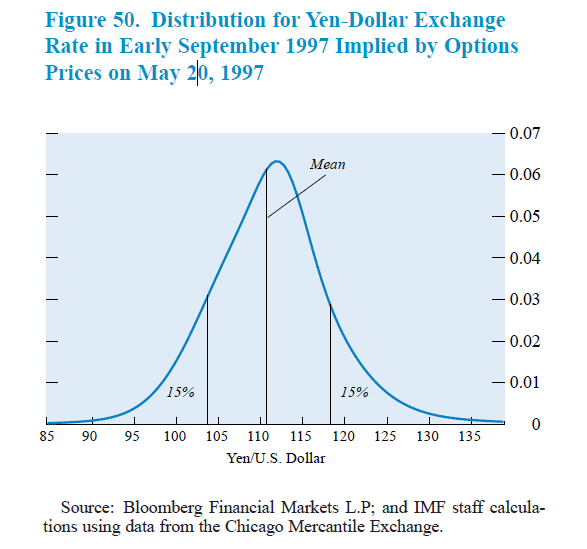
\includegraphics[width=0.8\linewidth]{images/figJPYRND} 

}

\caption{It was 20 years ago today: IMF, Capital Markets Report, 1997}\label{fig:fig-CMReport}
\end{figure}

She asked Huff Vihn, the author of the box, for a coffee meeting to
discuss information extraction from options. During the meeting, Vihn
could only talk about three options: 50, 75, and 85. They were
irrelevant to Payne, who was in the flower of her youth. But she could
not get much information from Vihn. He had been eating only mushrooms
during the past seven years. As Timothy Leary noted, a fungi-edible diet
could wreak havoc in somebody's deep neural networks.

Fortunately, Vihn had kept a copy of his data retrieval file and
promised to send it to Payne as soon as he was done with an important
memorandum. Vihn warned Payne that all the data in the files
corresponded to European instruments. Payne was perplexed: ``Don't they
trade in New York also?''. Vihn smiled and clarified that European
contracts could only be exercised at the contract maturity, which was
exactly the situation for the IMF 50, 75, and 85 options. Payne made a
note to read more about that.

The next morning, Payne got the file and an set of charts. ``Not bad for
a two dollar investment in coffee, I knew I could use the geezer'' she
thought to herself. Payne rushed to update the file in the committee's
Reuters terminal, soon to be decommissioned due to budget reallocation
priorities. Following good data practices, she then stored the data in a
human-readable \texttt{csv} file.

\section{Examining the data}\label{Data_exploration}

Payne used \texttt{RStudio} to analyze the data. ``How wonderful! A
great package for a great price! Zero !!''. She first loaded a number of
useful libraries, and an auxiliary source file using the following
commands:

\begin{Shaded}
\begin{Highlighting}[]
\KeywordTok{rm}\NormalTok{(}\DataTypeTok{list=}\KeywordTok{ls}\NormalTok{())             }\CommentTok{# Clean up memory}
\KeywordTok{library}\NormalTok{(ggplot2)          }\CommentTok{# Graphic library}
\KeywordTok{library}\NormalTok{(lubridate)        }\CommentTok{# Date manipulation library}
\KeywordTok{library}\NormalTok{(dplyr)            }\CommentTok{# Auxiliary functions for data manipulation}
\KeywordTok{source}\NormalTok{(}\StringTok{"auxFunctions.R"}\NormalTok{)  }\CommentTok{# Auxiliary functions for this chapter}
\end{Highlighting}
\end{Shaded}

Afterwards, it was a piece of cake to read the data file, and convert
the dates to a format the graphics library \texttt{ggplot2} could
understand:

\begin{Shaded}
\begin{Highlighting}[]
\NormalTok{filename =}\StringTok{ "2018_IET_Options_data.csv"}
\NormalTok{data =}\StringTok{ }\KeywordTok{read.csv}\NormalTok{(filename, }\DataTypeTok{header=}\OtherTok{TRUE}\NormalTok{)}
\NormalTok{data}\OperatorTok{$}\NormalTok{Dates =}\StringTok{ }\KeywordTok{mdy_hm}\NormalTok{(}\KeywordTok{as.character}\NormalTok{(data}\OperatorTok{$}\NormalTok{Dates))}
\end{Highlighting}
\end{Shaded}

The data file contained weekly mid-prices for a number of financial
variables, as shown below:

\begin{figure}
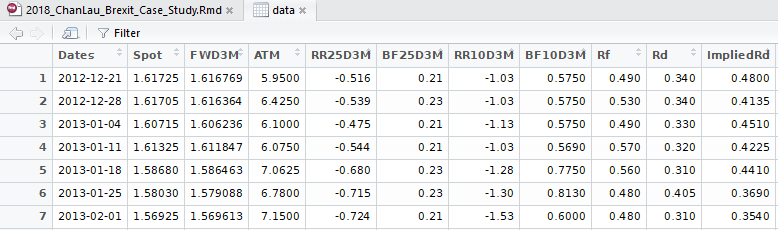
\includegraphics[width=1\linewidth]{images/figDataStructure} \caption{Data frame structure}\label{fig:unnamed-chunk-7}
\end{figure}

Some of the variables were easy to interpret:

\begin{itemize}
\tightlist
\item
  Spot: the GBPUSD spot exchange rate, i.e.~USD per GBP
\item
  FWD3M: the 3-month GBPUSD forward exchange rate
\item
  Rf: the 3-month GBP money market deposit rate, annualized (in percent)
\item
  Rd: the 3-month USD money market deposit rate, annualized (in percent)
\end{itemize}

Others were related to currency options, all with a 3-month maturity

\begin{itemize}
\tightlist
\item
  ATM: the at-the-money implied volatility of a GBPUSD option with
  strike price equal to spot
\item
  RR25D3M: the price of a 25\(\Delta\) risk reversal, in annualized
  volatility units (in percent)
\item
  BF25D3M: the price of a 25\(\Delta\) butterfly spread, in annualized
  volatility units (in percent)
\item
  RR10D3M: the price of a 10\(\Delta\) risk reversal, in annualized
  volatility units (in percent)
\item
  BF10D3M: the price of a 10\(\Delta\) butterfly spread, in annualized
  volatility units (in percent)
\end{itemize}

The final variable, \texttt{ImpliedRd}, was the 3-month USD money market
deposit rate implied from the forward rate, obtained from the covered
interest rate parity equation:

\[ F = S \frac{\exp \left(\text{Implied } R_d \times T\right)}{\exp \left(R_f \times T\right)} \]

where \(F\) is the forward exchange rate, \(S\) is the spot exchange
rate, \(R_x, x= f, d\) denotes the foreign and domestic deposit rates,
and \(T\) is the time to maturity of the option. For the purpose of the
analysis, the British pound is the foreign currency and the US dollar is
the domestic currency. To see this, note that the British pound is the
base currency or underlying asset since its price is given in US
dollars, the numeraire currency.

\section{Spot exchange rate}\label{spot-exchange-rate}

It was time to start eyeballing the data. First, she looked at the
dynamics of the spot and forward exchange rate highlighting carefully
the week of the Brexit referendum vote:

\begin{Shaded}
\begin{Highlighting}[]
\CommentTok{# Plot of the spot exchange rate with vertical line at Brexit vote}
\NormalTok{p1 =}\StringTok{ }\KeywordTok{ggplot}\NormalTok{(data, }\KeywordTok{aes}\NormalTok{(Dates, Spot)) }\OperatorTok{+}\StringTok{ }\KeywordTok{geom_line}\NormalTok{(}\DataTypeTok{colour=}\StringTok{"blue"}\NormalTok{) }
\NormalTok{p1 =}\StringTok{ }\NormalTok{p1 }\OperatorTok{+}\StringTok{ }\KeywordTok{geom_vline}\NormalTok{(}\DataTypeTok{xintercept=}\KeywordTok{as.POSIXct}\NormalTok{(}\KeywordTok{as.Date}\NormalTok{((}\StringTok{"2016-06-22 UTC"}\NormalTok{))),}\DataTypeTok{linetype=}\StringTok{"longdash"}\NormalTok{)}

\NormalTok{p2 =}\StringTok{ }\KeywordTok{ggplot}\NormalTok{(data, }\KeywordTok{aes}\NormalTok{(Dates, FWD3M)) }\OperatorTok{+}\StringTok{ }\KeywordTok{geom_line}\NormalTok{(}\DataTypeTok{colour=}\StringTok{"red"}\NormalTok{) }
\NormalTok{p2 =}\StringTok{ }\NormalTok{p2 }\OperatorTok{+}\StringTok{ }\KeywordTok{geom_vline}\NormalTok{(}\DataTypeTok{xintercept=}\KeywordTok{as.POSIXct}\NormalTok{(}\KeywordTok{as.Date}\NormalTok{((}\StringTok{"2016-06-22 UTC"}\NormalTok{))),}\DataTypeTok{linetype=}\StringTok{"longdash"}\NormalTok{)}

\KeywordTok{multiplot}\NormalTok{(p1,p2,}\DataTypeTok{cols=}\DecValTok{1}\NormalTok{)}
\end{Highlighting}
\end{Shaded}

\begin{figure}
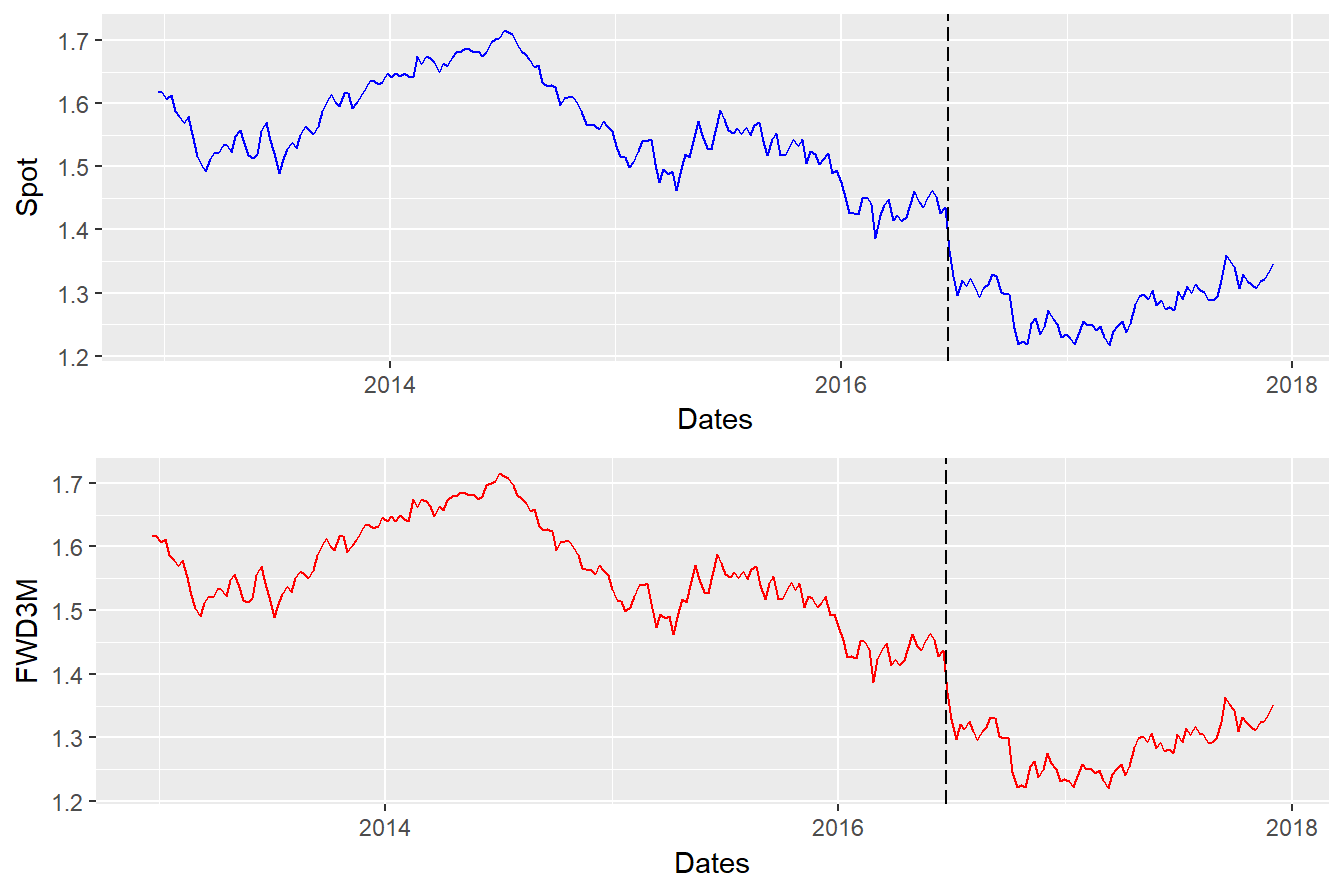
\includegraphics[width=1\linewidth]{images/unnamed-chunk-8-1} \caption{USDGBP spot and forward exchange rate}\label{fig:unnamed-chunk-8}
\end{figure}

The behavior of both series were quite similar. Both the spot and
forward rates had been range bound in the first half of 2016 and their
behavior did not anticipate the exchange rate correction following the
referendum. Payne proceed to analyze the other data series hoping they
could provide additional information.

\section{Implied and actual USD
rates}\label{implied-and-actual-usd-rates}

A cursory glimpse of the data had shown that the actual USD deposit rate
was different from the rate implied from the forward exchange rate.
Payne examined this, by first calculating the rate spread:

\begin{Shaded}
\begin{Highlighting}[]
\NormalTok{data}\OperatorTok{$}\NormalTok{spreadRd =}\StringTok{ }\NormalTok{(data}\OperatorTok{$}\NormalTok{ImpliedRd }\OperatorTok{-}\StringTok{ }\NormalTok{data}\OperatorTok{$}\NormalTok{Rd)}\OperatorTok{*}\DecValTok{100}
\NormalTok{p3 =}\StringTok{ }\KeywordTok{ggplot}\NormalTok{(data, }\KeywordTok{aes}\NormalTok{(Dates, spreadRd)) }\OperatorTok{+}\StringTok{ }\KeywordTok{geom_line}\NormalTok{(}\DataTypeTok{colour=}\StringTok{"purple"}\NormalTok{) }\OperatorTok{+}\StringTok{ }\KeywordTok{geom_hline}\NormalTok{(}\DataTypeTok{yintercept=}\DecValTok{0}\NormalTok{)}
\NormalTok{p3 =}\StringTok{ }\NormalTok{p3 }\OperatorTok{+}\StringTok{ }\KeywordTok{geom_vline}\NormalTok{(}\DataTypeTok{xintercept=}\KeywordTok{as.POSIXct}\NormalTok{(}\KeywordTok{as.Date}\NormalTok{((}\StringTok{"2016-06-22 UTC"}\NormalTok{))),}\DataTypeTok{linetype=}\StringTok{"longdash"}\NormalTok{)}
\NormalTok{p3}
\end{Highlighting}
\end{Shaded}

\begin{figure}
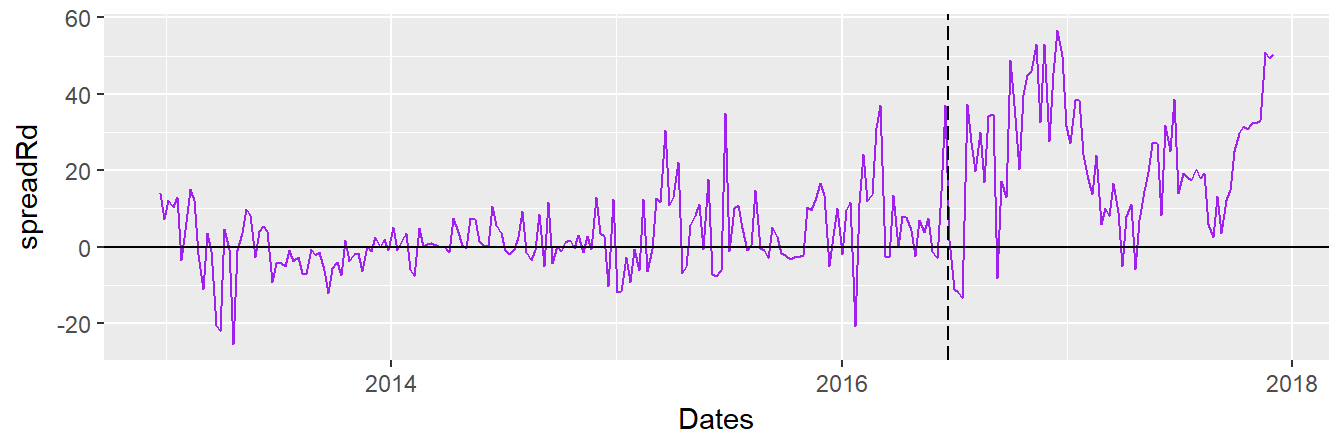
\includegraphics[width=1\linewidth]{images/unnamed-chunk-9-1} \caption{Implied and current 3-month USD deposit rate differential, in bps}\label{fig:unnamed-chunk-9}
\end{figure}

This was an interesting finding. Currency forwards, in combination with
spot currency transactions and borrowing, are useful to create synthetic
loans, as the diagram below shows:

\hypertarget{synthetic-USD-loan}{}
\begin{figure}
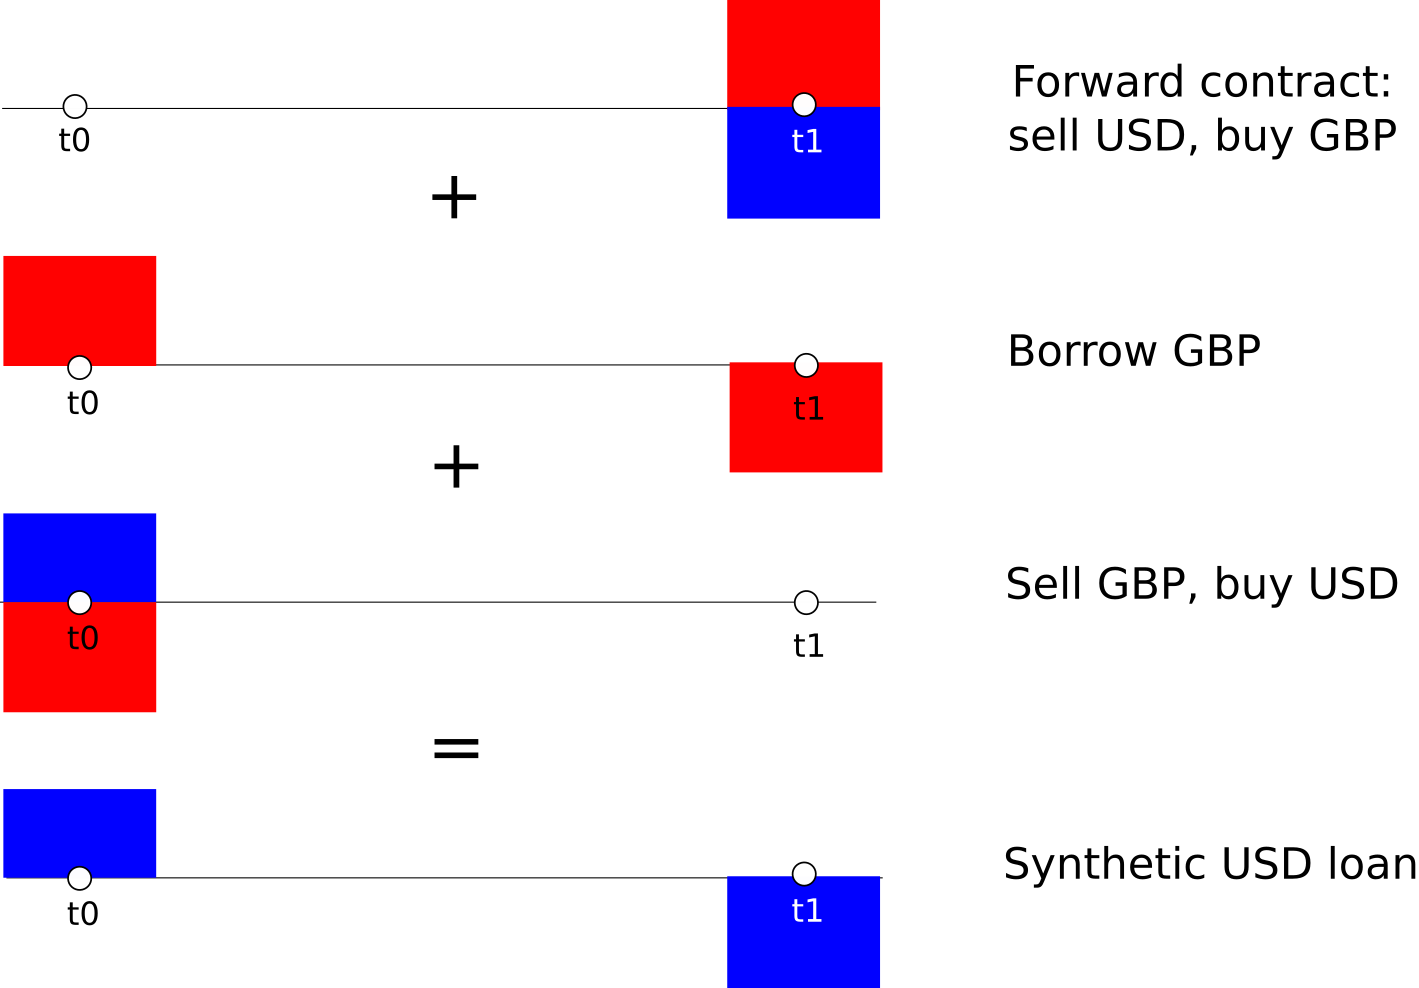
\includegraphics[width=0.7\linewidth]{images/figSyntheticUSDLoan} \caption{Synthetic USD loan}\label{fig:unnamed-chunk-10}
\end{figure}

In principle, there should not be major differences between the deposit
rate and the synthetic loan rate. Whenever the implied USD rate exceeds
the USD deposit rate, a covered interest parity violation, it signals a
strong demand for USD satisfied mainly via the synthetic market rather
than the cash market. If the rate differential is large and persistent,
and above historically levels, it may reflect frictions and liquidity
shortages preventing cross-market arbitrage.

Payne observed that before 2015, the 3-month rate differential was small
and exhibited low volatility. Starting 2015, the volatility of the rate
differential increased, with covered interest parity violations favoring
the synthetic US dollar rate. In many instances, the synthetic rate
could exceed the cash market rate by as much as 40 bps. Violations,
however were short-lived.

In the post-Brexit period, deviations became larger and more persistent.
At one moment, the synthetic and the cash rates were even, roughly
coinciding with the Tories' loss of their parliamentary majority in June
2017. The loss likely sparked hopes that the Brexit process may be
halted or reverted. Since the last quarter of 2017, however, the gap
between the synthetic and cash rates have widened. Based on the November
2017 Bank of England \emph{Inflation Report}, Payne considered downward
revisions of UK growth prospects and Brexit uncertainty were driving
appetite for USD assets, leading to the recent widening of the implied
USD rate spread.

\section{ATM option volatility}\label{atm-option-volatility}

Payne was not very familiar with currency options. She called Stan Ford,
an old classmate who was a FX strategist in London, to get some hints.
Unfortunately, nobody picked up the phone. Unbeknownst to her, the firm
had replaced Stan with an impressive Asian ML/AI trading system,
\emph{UZakAIDon}. Depressed, Stan had checked into solitary confinement
in an Italian monastery. So she picked up an old derivatives textbooks
somebody had left in the bookcases outside her closet office. Although
old, it looked like new as the shrink wrap had never been removed. She
went straight to the chapter on options and looked at the payoff of an
European call option at maturity:

\hypertarget{figure-call-option}{}
\begin{figure}
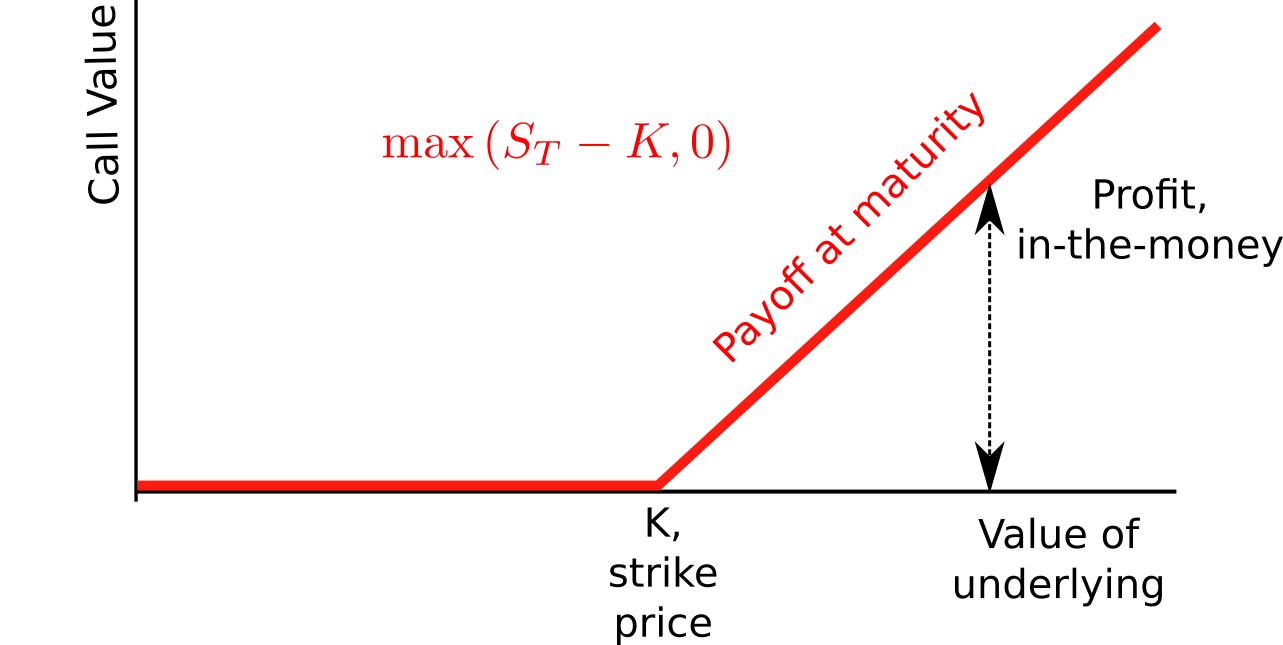
\includegraphics[width=0.7\linewidth]{images/figCallOptionMaturity} \caption{Call option payoff at maturity}\label{fig:unnamed-chunk-11}
\end{figure}

At maturity, the option buyer, who is long the call, has the right to
exercise the option. If he does, he receives a payoff equal to
\(S_T -K\). Clearly, exercising the option makes sense only when the
value of the underlying is above the strike price the option is said to
be in the money \emph{in-the-money} (ITM). More generally, the option is
\emph{ITM} whenever the spot price is above the strike price, regardless
of the time to maturity. When the value of the underlying is equal to
the strike price, the option is \emph{at-the-money} (ATM) Otherwise, it
is \emph{out of the money} (OTM). For the GBPUSD options, the underlying
is the British pound, which is quoted as the amount of US dollars needed
to buy one pound, or the GBPUSD exchange rate. The call option is worth
more when the pound appreciates against the dollar.

There were some tedious formulas and derivations related to the pricing
of the options. Payne found the math insufferable. She had accepted the
job at the IMF because her comparative advantage was policy making. In
fact, she never appreciated the ``mathiness'' environment prevalent in
graduate school. Payne felt a jolt of relief when she encountered a
passage in the book stating that \textbf{dealers quoted currency option
prices as implied volatility, or \emph{vols}}. ``Hence, all I need to do
now is check what happens to the vols!''

An examination of the call option chart provided some support for the
market practice: for an OTM option, higher volatility implies a greater
chance that the option ends ITM. For an ITM option, higher volatility
implies higher payoffs while the downside risk is limited to losing the
option premium.The higher the vol, the more expensive the currency
option is.

The book also noted that to obtain prices, the vol should be input into
the benchmark Garman-Kolhagen currency option pricing model.\footnote{\citet{Garman-Kohlhagen1983}}
This model, in turn, was derived from another one that explains the
emergence of black holes in the universe, the celebrated
Black-Scholes-Merton model.\footnote{\citet{Black-Scholes1973} and
  \citet{Merton1973}}

``I would check the theory later,'' Payne mumbled to herself while
plotting the ATM volatility:

\begin{Shaded}
\begin{Highlighting}[]
\NormalTok{p4 =}\StringTok{ }\KeywordTok{ggplot}\NormalTok{(data, }\KeywordTok{aes}\NormalTok{(Dates, ATM)) }\OperatorTok{+}\StringTok{ }\KeywordTok{geom_line}\NormalTok{(}\DataTypeTok{colour=}\StringTok{"blue"}\NormalTok{) }\OperatorTok{+}\StringTok{ }\KeywordTok{geom_hline}\NormalTok{(}\DataTypeTok{yintercept=}\DecValTok{0}\NormalTok{)}
\NormalTok{p4 =}\StringTok{ }\NormalTok{p4 }\OperatorTok{+}\StringTok{ }\KeywordTok{geom_vline}\NormalTok{(}\DataTypeTok{xintercept=}\KeywordTok{as.POSIXct}\NormalTok{(}\KeywordTok{as.Date}\NormalTok{((}\StringTok{"2016-06-22 UTC"}\NormalTok{))),}\DataTypeTok{linetype=}\StringTok{"longdash"}\NormalTok{)}
\NormalTok{p4}
\end{Highlighting}
\end{Shaded}

\begin{figure}
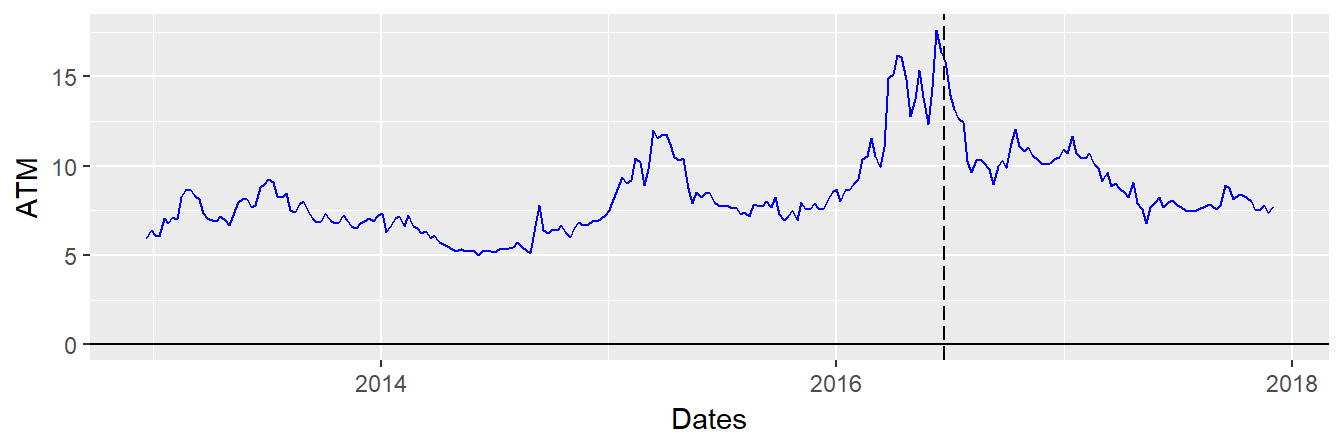
\includegraphics[width=1\linewidth]{images/unnamed-chunk-12-1} \caption{ATM volatility}\label{fig:unnamed-chunk-12}
\end{figure}

The chart showed that ATM volatility increased rapidly during the first
half of 2016, but slumped rapidly after Brexit. During most of 2017 it
had been in a narrow range, reflecting the range-like behavior of the
exchange rate.

The chart was somewhat puzzling. Apparently, options became more
valuable in the months before the referendum. A more valuable call
option seemingly implied a higher exchange rate, or an appreciation of
the GBP against the USD. But this assertion was at odds with the
behavior of the implied and actual USD rates. The solution to this
puzzle was rather simple: put options also benefit from higher
volatility.

\begin{figure}
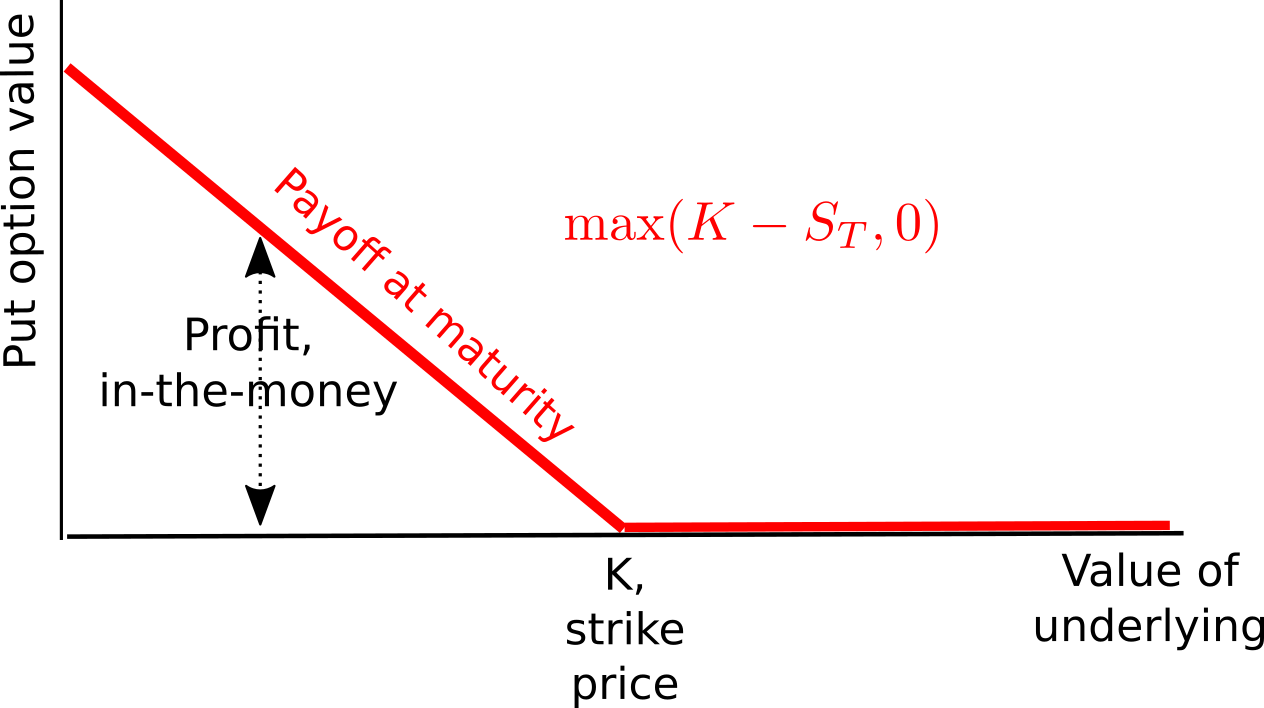
\includegraphics[width=0.7\linewidth]{images/figPUtOptionMaturity} \caption{Put option payoff at maturity}\label{fig:unnamed-chunk-13}
\end{figure}

For an OTM option, higher volatility could push the exchange rate down,
i.e.~the pound depreciates against the dollar, forcing the option to be
in the ITM. The downside is limited to losing the option premium. In
contrast to the call option, upside gains are capped. But the buyer of
the put still benefits more from increased volatility. We can conclude
that ATM volatility is not enough to capture the market's view on the
direction of exchange rate changes. In contrast to academic textbooks, a
number of market practitioners would attest that plain options are
instruments for expressing views on volatility and not on market
direction.\footnote{\citet{Derman-Miller2016}}

\section{Risk Reversals}\label{risk-reversals}

To assess directional views, it is necessary to look at risk reversals,
a particular combination of simpler options. The options book, being
old, did not say anything about risk reversals. Thankfully, the Google
had offered the Home at a discount price during last Black Friday. Payne
asked her Google Home what a risk reversal was and obtained the
following answer from Wikipedia:

\begin{figure}
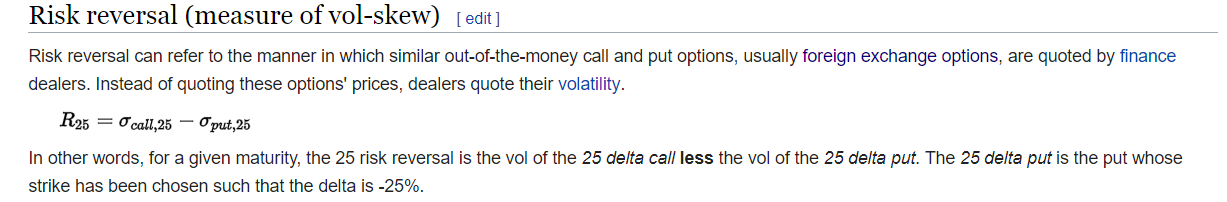
\includegraphics[width=1\linewidth]{images/figRRDefinition} \caption{Risk reversal definition (Wikipedia)}\label{fig:unnamed-chunk-14}
\end{figure}

A full understanding of the risk reversal requires knowing what
\(\Delta\) is. Even without that knowledge, however, we can use risk
reversal quotes to assess the prices market participants place on
potential exchange rate movements. Let's start with the price quote of a
risk reversal:

\[
RR_{25\Delta} = \sigma_{25\Delta C} - \sigma_{25\Delta P}
\]

We pay \(\sigma_{25\Delta C}\) for owning the call and offset this cost
somewhat by selling the put at \(\sigma_{25\Delta P}\). At maturity, the
payoff diagram of the risk reversal, long a call and short a put, both
of them OTM, is:

\begin{figure}
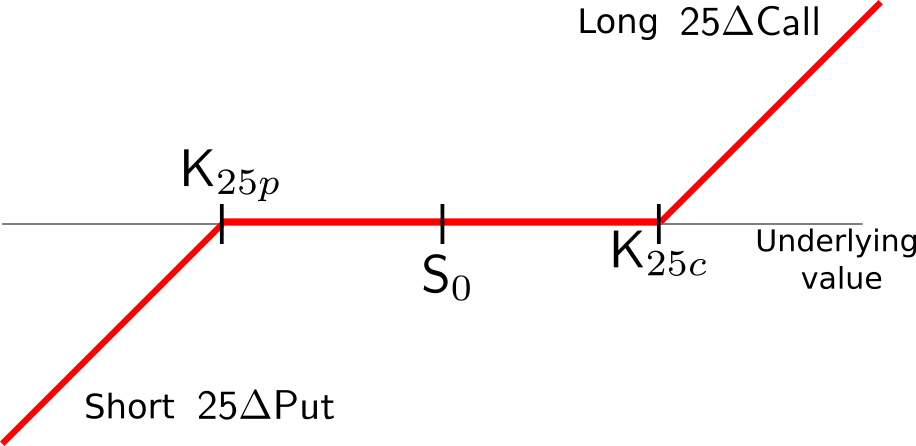
\includegraphics[width=0.7\linewidth]{images/fig25RRSimple} \caption{Risk reversal payoff at maturity}\label{fig:unnamed-chunk-15}
\end{figure}

When the call is more valuable than the put, the value of the risk
reversal is positive. The buyer of the risk reversal values more events
in which the GBPUSD exchange rate goes up. The opposite is true when the
risk reversal is negative, i.e.~the put is more valuable than the call.
Risk reversals reveals potential asymmetries affecting exchange rate
movements. In the case of the British pound, bullish market views are
reflected in positive risk reversals. On the other hand, bearish views
are reflected in negative risk reversals. Payne plotted both the
25\(\Delta\) and 10\(\Delta\) risk reversals:

\begin{Shaded}
\begin{Highlighting}[]
\NormalTok{p5 =}\StringTok{ }\KeywordTok{ggplot}\NormalTok{(data, }\KeywordTok{aes}\NormalTok{(Dates, RR25D3M)) }\OperatorTok{+}\StringTok{ }\KeywordTok{geom_line}\NormalTok{(}\DataTypeTok{colour=}\StringTok{"red"}\NormalTok{) }\OperatorTok{+}\StringTok{ }\KeywordTok{geom_hline}\NormalTok{(}\DataTypeTok{yintercept=}\DecValTok{0}\NormalTok{)}
\NormalTok{p5 =}\StringTok{ }\NormalTok{p5 }\OperatorTok{+}\StringTok{ }\KeywordTok{geom_vline}\NormalTok{(}\DataTypeTok{xintercept=}\KeywordTok{as.POSIXct}\NormalTok{(}\KeywordTok{as.Date}\NormalTok{((}\StringTok{"2016-06-22 UTC"}\NormalTok{))),}\DataTypeTok{linetype=}\StringTok{"longdash"}\NormalTok{)}

\NormalTok{p6 =}\StringTok{ }\KeywordTok{ggplot}\NormalTok{(data, }\KeywordTok{aes}\NormalTok{(Dates, RR10D3M)) }\OperatorTok{+}\StringTok{ }\KeywordTok{geom_line}\NormalTok{(}\DataTypeTok{colour=}\StringTok{"blue"}\NormalTok{) }\OperatorTok{+}\StringTok{ }\KeywordTok{geom_hline}\NormalTok{(}\DataTypeTok{yintercept=}\DecValTok{0}\NormalTok{)}
\NormalTok{p6 =}\StringTok{ }\NormalTok{p6 }\OperatorTok{+}\StringTok{ }\KeywordTok{geom_vline}\NormalTok{(}\DataTypeTok{xintercept=}\KeywordTok{as.POSIXct}\NormalTok{(}\KeywordTok{as.Date}\NormalTok{((}\StringTok{"2016-06-22 UTC"}\NormalTok{))),}\DataTypeTok{linetype=}\StringTok{"longdash"}\NormalTok{)}
\KeywordTok{multiplot}\NormalTok{(p5, p6, }\DataTypeTok{cols=}\DecValTok{1}\NormalTok{)}
\end{Highlighting}
\end{Shaded}

\begin{figure}
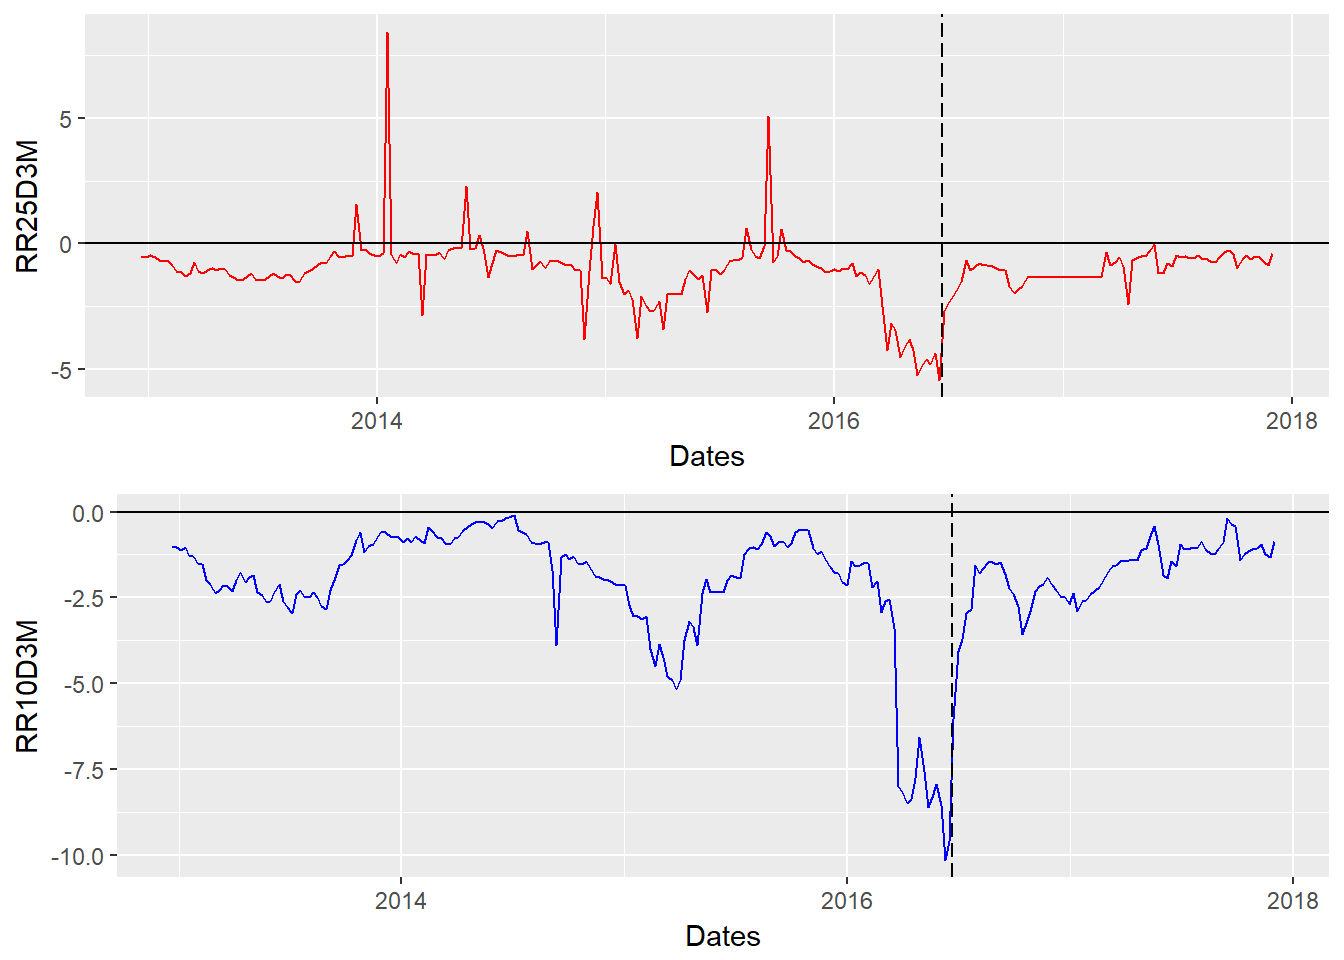
\includegraphics[width=1\linewidth]{images/unnamed-chunk-16-1} \caption{GBPUSD Risk reversals}\label{fig:unnamed-chunk-16}
\end{figure}

Since 2013, risk reversals had been negative. There were some brief
periods during which the 25\(\Delta\) risk reversals turned positive.
During the first half of 2016 both the 10\(\Delta\) and the 25\(\Delta\)
risk reversals dropped substantially as markets placed more weight on
the depreciation of the pound than on its appreciation. In combination
with the ATM vol, the dramatic widening of the risk reversals
anticipated the sharp exchange rate correction following the Brexit
referendum.

\section{Butterfly spreads}\label{butterfly-spreads}

``Quite interesting,'' thought Payne. ``Regardless of its perceived lack
of ethics, creativity in the financial industry abounds.'' She wondered
what instrument could be useful for an investor expecting the exchange
rate to experience either large movements on the upside or the downside.
Remembering the risk reversal payoff chart, she concluded that it was a
simple as flipping the short put position over the horizontal axis. That
is, holding both a long OTM call and a long OTM put position should do
the trick. She drew this chart, keeping the strikes of the put and the
call at the values they had in the risk reversal:

\begin{figure}
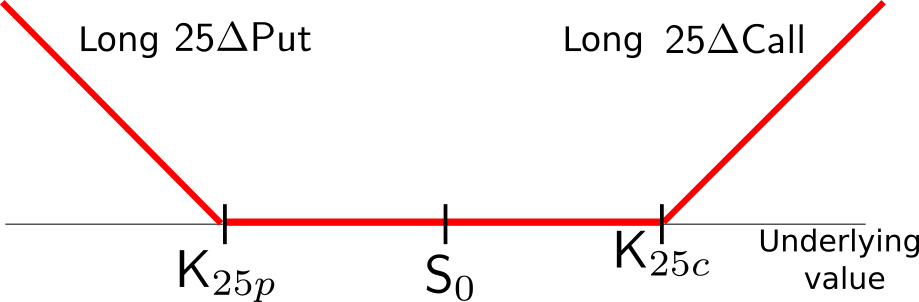
\includegraphics[width=0.7\linewidth]{images/fig25BFSimple} \caption{Strangle payoff at maturity}\label{fig:unnamed-chunk-17}
\end{figure}

Payne had just re-discovered the \textbf{strangle}. This instrument
typically delivers a positive payoff when the underlying is very
volatile. For instance, speculators use strangles to position themselves
ahead of earning releases. Missing or exceeding earning expectations
trigger large downside and upside movements in the stock price,
benefiting strangle holders.

Using the same convention as for the risk reversals, the price of a
25\(\Delta\) strangle is:

\[
S_{25\Delta} = \sigma_{25\Delta C} + \sigma_{25\Delta P}
\]

The only glitch, however, was that the quoted prices were for butterfly
spreads. FX dealers quote the price of a 25\(\Delta\) butterfly spread
as:

\[
BF_{25\Delta} = \frac{\sigma_{25\Delta C} + \sigma_{25\Delta P}}{2}  - \sigma_{ATM}
\]

``This is very annoying but there must be a meaning to this
convention,'' Payne whispered to herself. Suddenly, she remembered what
Stan, the now vanished FX trader, used to say: ``We never put our own
money in the trades.'' Examining the risk reversal again, she realized
that its cost, \(\sigma_{25\Delta C} - \sigma_{25\Delta P}\) had to be
lower than buying a simple call \(\sigma_{25\Delta C}\). The sale of the
put offset the purchase price of the call.

For the strangle, she needed to buy both the call and the put. ``How
would I offset that? By selling two ATM options, of course!'' she
exclaimed. ``What a strange convention but it does make a lot of sense''
whispered Payne to herself. To understand better why FX dealers would
prefer the butterfly to the strangle, Payne draw two diagrams, unaware
that she was taking the first steps toward unlocking the concept of the
volatility smile:

\begin{figure}
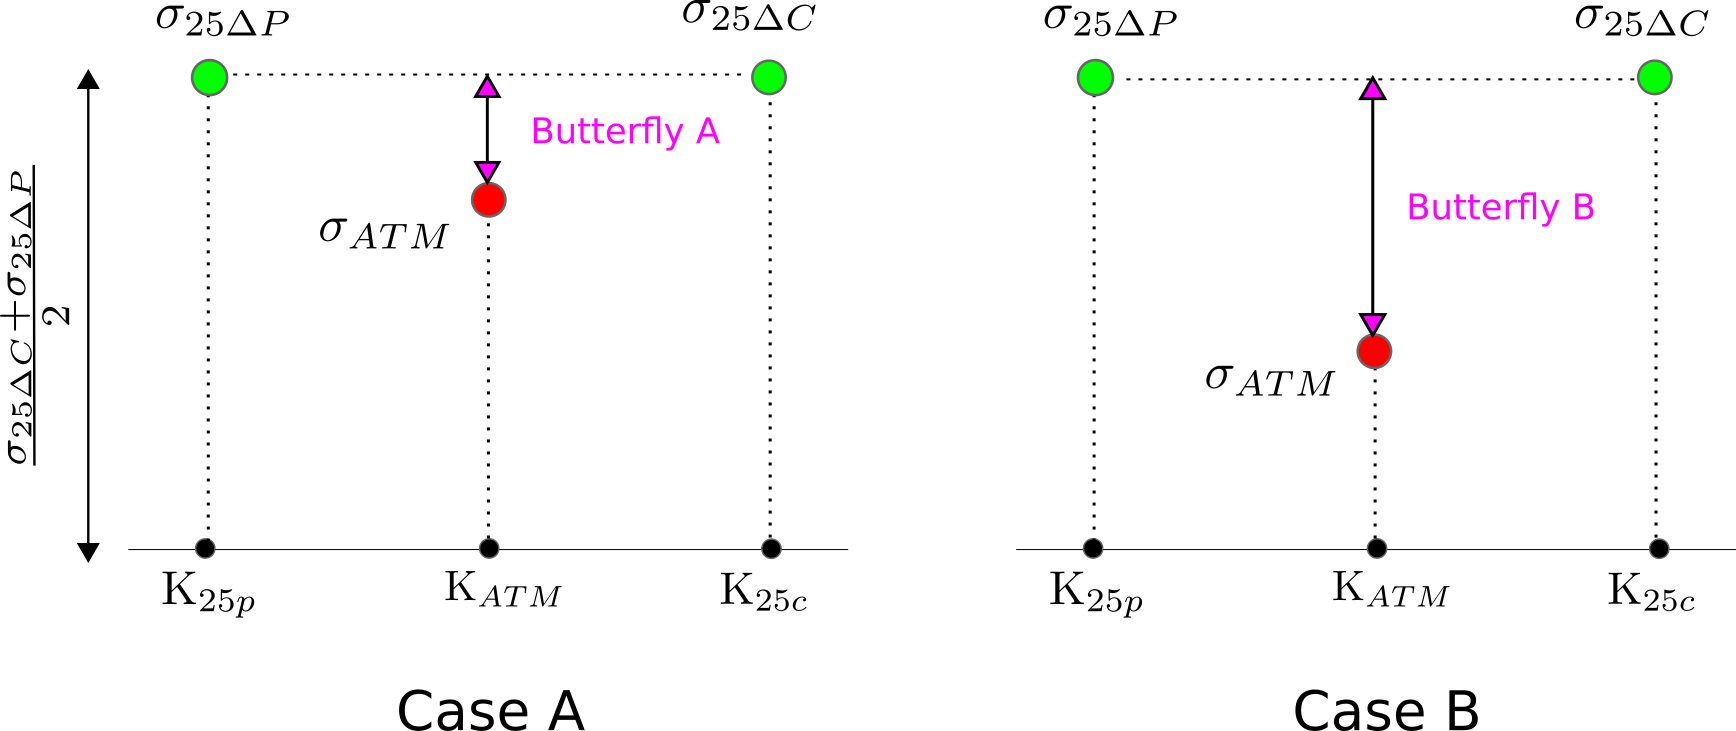
\includegraphics[width=1\linewidth]{images/figStrangleButterfly} \caption{Strangles vs. butterflies}\label{fig:unnamed-chunk-18}
\end{figure}

In both cases, the value of the strangle is the same and equal to
\(\sigma_{25\Delta C} + \sigma_{25\Delta P}\). Taking half the strangle
price and subtracting the \(ATM\) vol yield different butterfly values
in cases A and B. Assuming roughly that the vols corresponded to the
weights markets placed on certain strike price values, it became clear
that the butterflies convey much more information than the strangles. In
case A, the market prices upside and downside movements only slightly
higher than the event that exchange rate stays close to the \(ATM\)
level. In contrast, in case B, the market places way more weight on the
events that the exchange rate will deviate substantially from the
\(ATM\) level.

She then plotted the butterfly quotes and obtained these charts:

\begin{Shaded}
\begin{Highlighting}[]
\NormalTok{p7 =}\StringTok{ }\KeywordTok{ggplot}\NormalTok{(data, }\KeywordTok{aes}\NormalTok{(Dates, BF25D3M)) }\OperatorTok{+}\StringTok{ }\KeywordTok{geom_line}\NormalTok{(}\DataTypeTok{colour=}\StringTok{"red"}\NormalTok{) }\OperatorTok{+}\StringTok{ }\KeywordTok{geom_hline}\NormalTok{(}\DataTypeTok{yintercept=}\DecValTok{0}\NormalTok{)}
\NormalTok{p7 =}\StringTok{ }\NormalTok{p7 }\OperatorTok{+}\StringTok{ }\KeywordTok{geom_vline}\NormalTok{(}\DataTypeTok{xintercept=}\KeywordTok{as.POSIXct}\NormalTok{(}\KeywordTok{as.Date}\NormalTok{((}\StringTok{"2016-06-22 UTC"}\NormalTok{))),}\DataTypeTok{linetype=}\StringTok{"longdash"}\NormalTok{)}

\NormalTok{p8 =}\StringTok{ }\KeywordTok{ggplot}\NormalTok{(data, }\KeywordTok{aes}\NormalTok{(Dates, BF10D3M)) }\OperatorTok{+}\StringTok{ }\KeywordTok{geom_line}\NormalTok{(}\DataTypeTok{colour=}\StringTok{"blue"}\NormalTok{) }\OperatorTok{+}\StringTok{ }\KeywordTok{geom_hline}\NormalTok{(}\DataTypeTok{yintercept=}\DecValTok{0}\NormalTok{)}
\NormalTok{p8 =}\StringTok{ }\NormalTok{p8 }\OperatorTok{+}\StringTok{ }\KeywordTok{geom_vline}\NormalTok{(}\DataTypeTok{xintercept=}\KeywordTok{as.POSIXct}\NormalTok{(}\KeywordTok{as.Date}\NormalTok{((}\StringTok{"2016-06-22 UTC"}\NormalTok{))),}\DataTypeTok{linetype=}\StringTok{"longdash"}\NormalTok{)}
\KeywordTok{multiplot}\NormalTok{(p7, p8, }\DataTypeTok{cols=}\DecValTok{1}\NormalTok{)}
\end{Highlighting}
\end{Shaded}

\begin{figure}
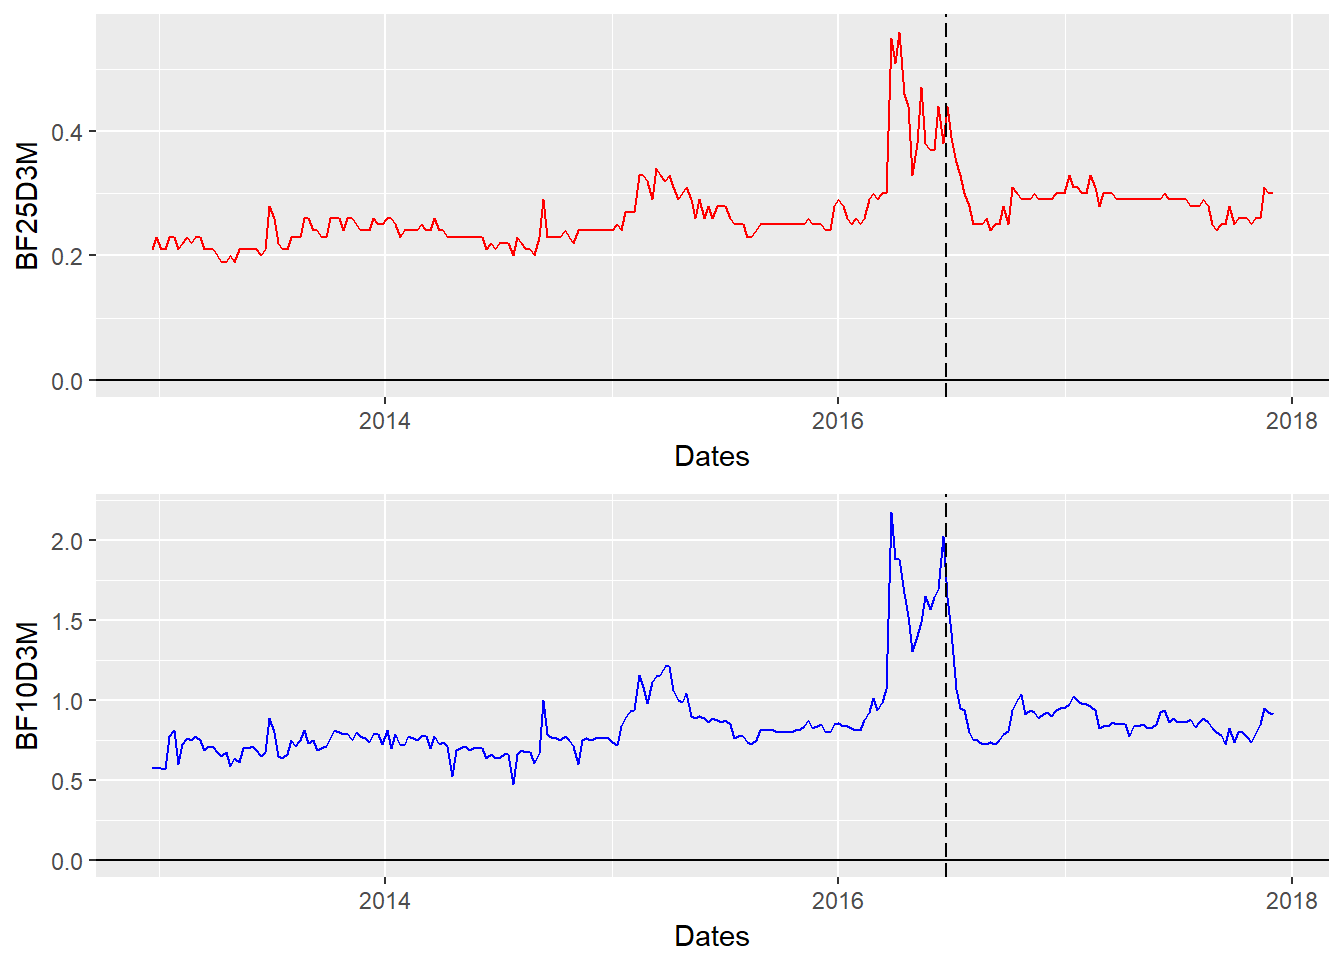
\includegraphics[width=1\linewidth]{images/unnamed-chunk-19-1} \caption{GBPUSD Butterflies}\label{fig:unnamed-chunk-19}
\end{figure}

From 2014 onward, butterfly quotes had been mostly range bound. The
notable exception was the first half of 2016, when butterfly quotes
reached record high levels three to four times the average level
observed in the previous three years. The combination of the \(ATM\)
vol, the risk reversals, and the butterflies was indeed revealing much
about market sentiment in the pre- and post- Brexit periods.

\chapter{A modicum of option pricing
theory}\label{a-modicum-of-option-pricing-theory}

Through her non-technical analysis, Payne had gained a deeper
understanding of the economic intuition of the pricing rationale of FX
options and their information content. But she had already reached the
stage where some basic option mathematics was necessary to understand
how best to squeeze the information out of currency options.

Pairing her Amazon Prime account with the newly acquired Alexa Amazon
device, bought at a bargain Black Friday price, she ordered some
derivatives books enjoying 2-day free delivery.\footnote{\citet{Wilmott2006}
  and \citet{Hull2017}.} When the books arrived, she started reading
them and taking notes. Let's take a discrete peek at these notes.

\section{\texorpdfstring{The \(\Delta\) of an
option}{The \textbackslash{}Delta of an option}}\label{the-delta-of-an-option}

The first concept requiring clarification is the \(\Delta\) of an
option. Simply speaking, the \(\Delta\) of an option measures the
sensitivity of the instrument to changes in the value of the underlying,
\(S\). For a call option, with price denoted as \(C\), its \(\Delta\)
is:

\[ \Delta_C = \frac{\partial C}{\partial S}.\]

Similarly, for a put the \(\Delta\) is:

\[ \Delta_P = \frac{\partial P}{\partial S}.\]

Note that the \(\Delta\) of a put is always negative. Hence, attention
should be paid when looking at option structures. In a risk reversal,
there is a short put. Hence, the \(\Delta\) of this put is positive. In
the strangle, there is a long put position and the \(\Delta\) is
negative. But the strike prices of these puts will always be referred to
as \(XY\Delta\), where \(XY\) is the absolute value of the \(\Delta\) of
the put option.

Armed with this knowledge, it is straightforward to link the \(\Delta\)s
in the risk reversal to their corresponding strike prices:

\begin{figure}
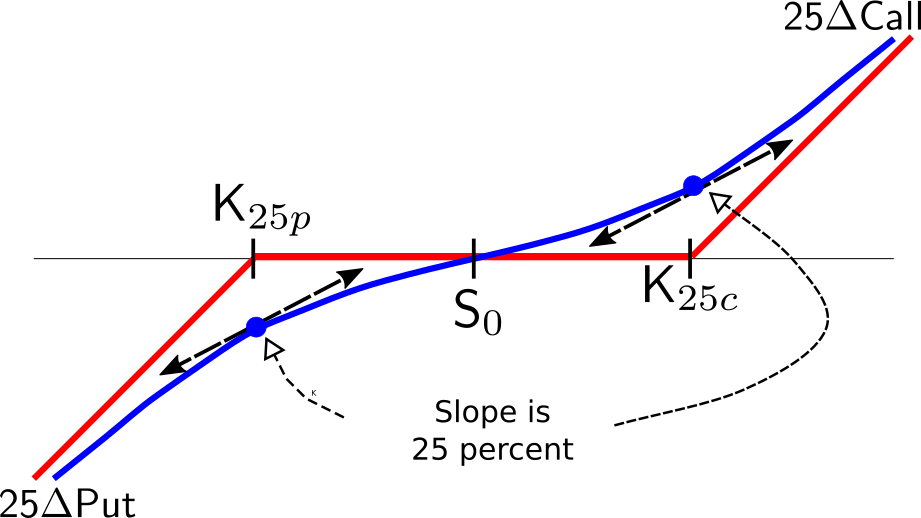
\includegraphics[width=0.6\linewidth]{images/fig25RR} \caption{25$\Delta$ risk reversal}\label{fig:unnamed-chunk-20}
\end{figure}

as well as in the strangle:

\begin{figure}
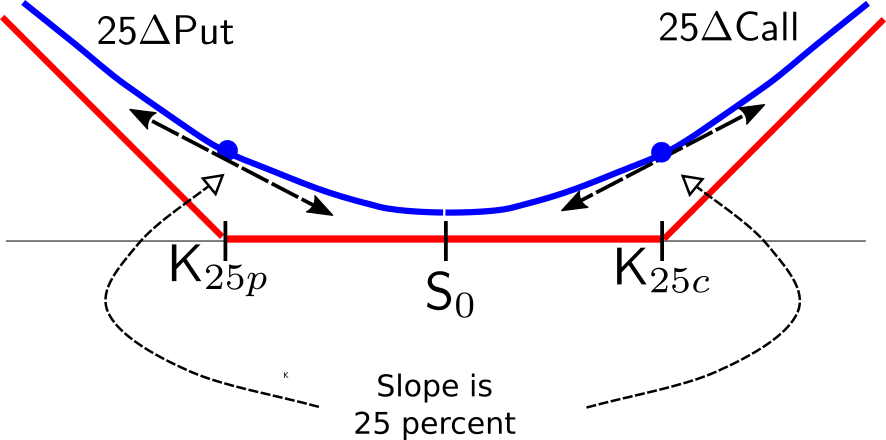
\includegraphics[width=0.6\linewidth]{images/fig25Strangle} \caption{25$\Delta$ strangle}\label{fig:unnamed-chunk-21}
\end{figure}

and to figure out the strike points for different \(\Delta\)s in a
single type of instrument:

\begin{figure}
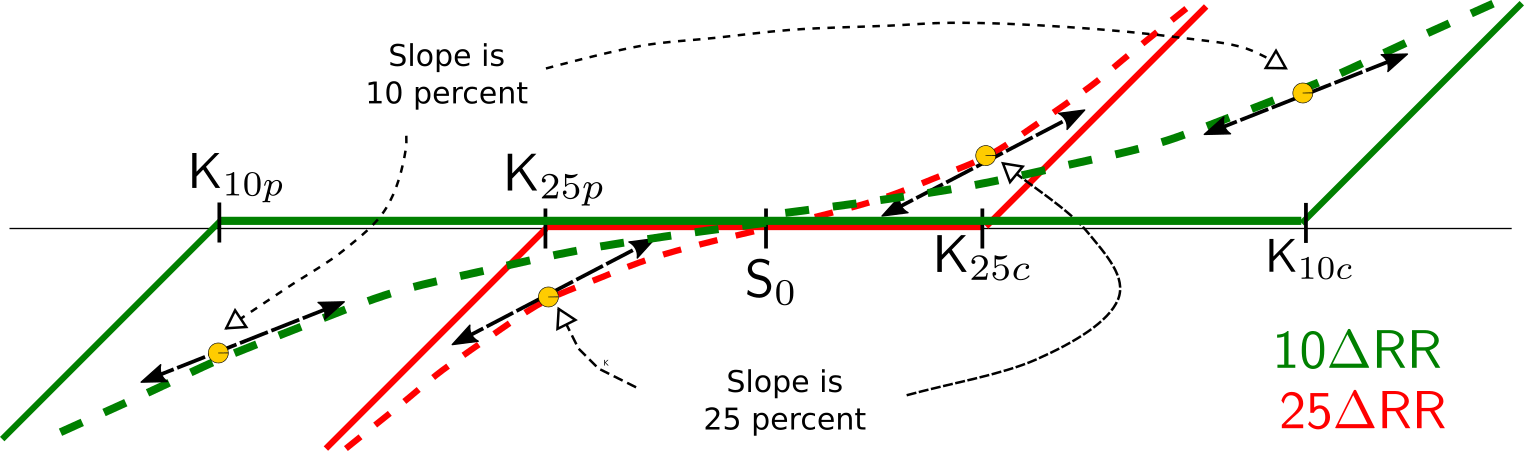
\includegraphics[width=0.8\linewidth]{images/fig1025RR} \caption{10$\Delta$ and 25$\Delta$ risk reversals}\label{fig:unnamed-chunk-22}
\end{figure}

The 10\(\Delta\) strike points are way more out-of-the money than the
25\(\Delta\) strike points. The quotes of the former can better capture
tail movements of the exchange rate. On the other hand, however, the
market is substantially more liquid for the 25\(\Delta\) options than
for the 10\(\Delta\) options. In some instances, the latter could
reflect not only the way the market weighs tail risk but a liquidity
premium as well.

The mathematics, examined in isolation, do not convey much intuition.
Rather, the \(\Delta\) of an option becomes important when placed in the
context of dynamic replication, as explained in the following box.

\section*{\texorpdfstring{Box 1. \(\Delta\) and dynamic
replication}{Box 1. \textbackslash{}Delta and dynamic replication}}\label{box-1.-delta-and-dynamic-replication}
\addcontentsline{toc}{section}{Box 1. \(\Delta\) and dynamic
replication}

Dynamic replication consists in constructing a portfolio of simpler
instruments that delivers the same payoff as an option. Several texts
describe in detail the mechanics of dynamic replication, with all its
mathematical bells and whistles. This box offers a simpler, more
intuitive explanation. Let's focus again on the payoff of a call option
(Figure 5), and compare it to the payoff of a forward contract with
strike price \(K\) and the same maturity as the option:

\begin{figure}
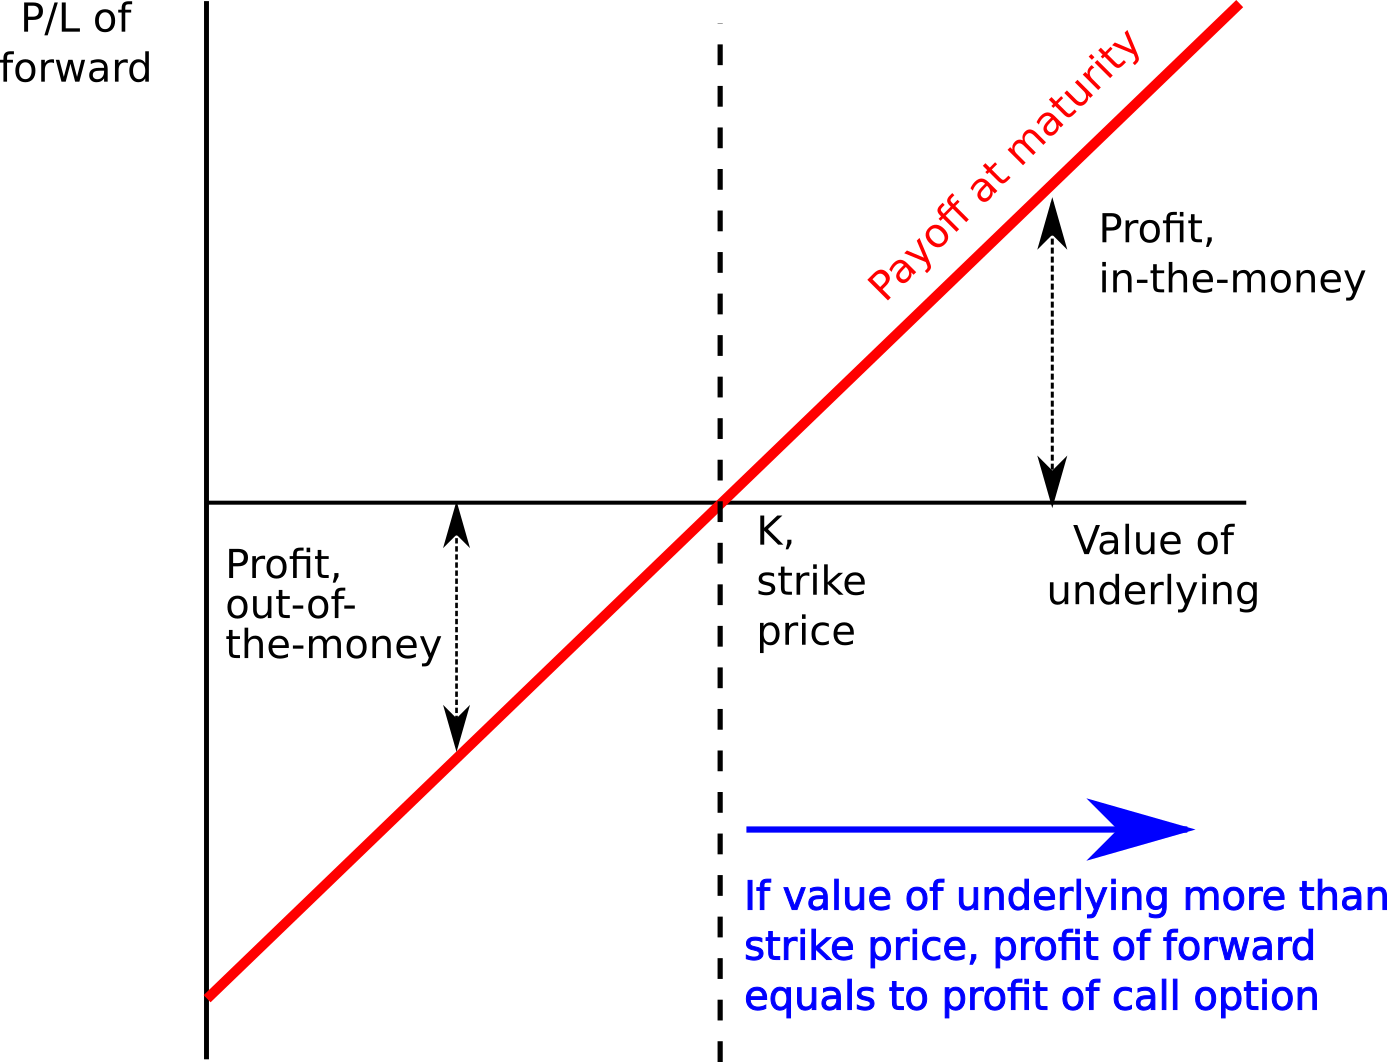
\includegraphics[width=0.6\linewidth]{images/figLongPosition} \caption{Payoff of a forward contract at maturity}\label{fig:unnamed-chunk-23}
\end{figure}

The payoff of the forward contract, at maturity, matches that of the
call option. Hence, whenever the value of the underlying, \(S\), exceeds
the strike price \(K\) at maturity, we are indifferent between holding
the call or the forward. What we are missing so far is an instrument
with the same payoff as the option when \(S < K\). Cash is the simple
instrument that does the trick, with a flat payoff at maturity. So we
would prefer to hold cash rather than the forward at maturity when
\(S < K\) at maturity:

\begin{figure}
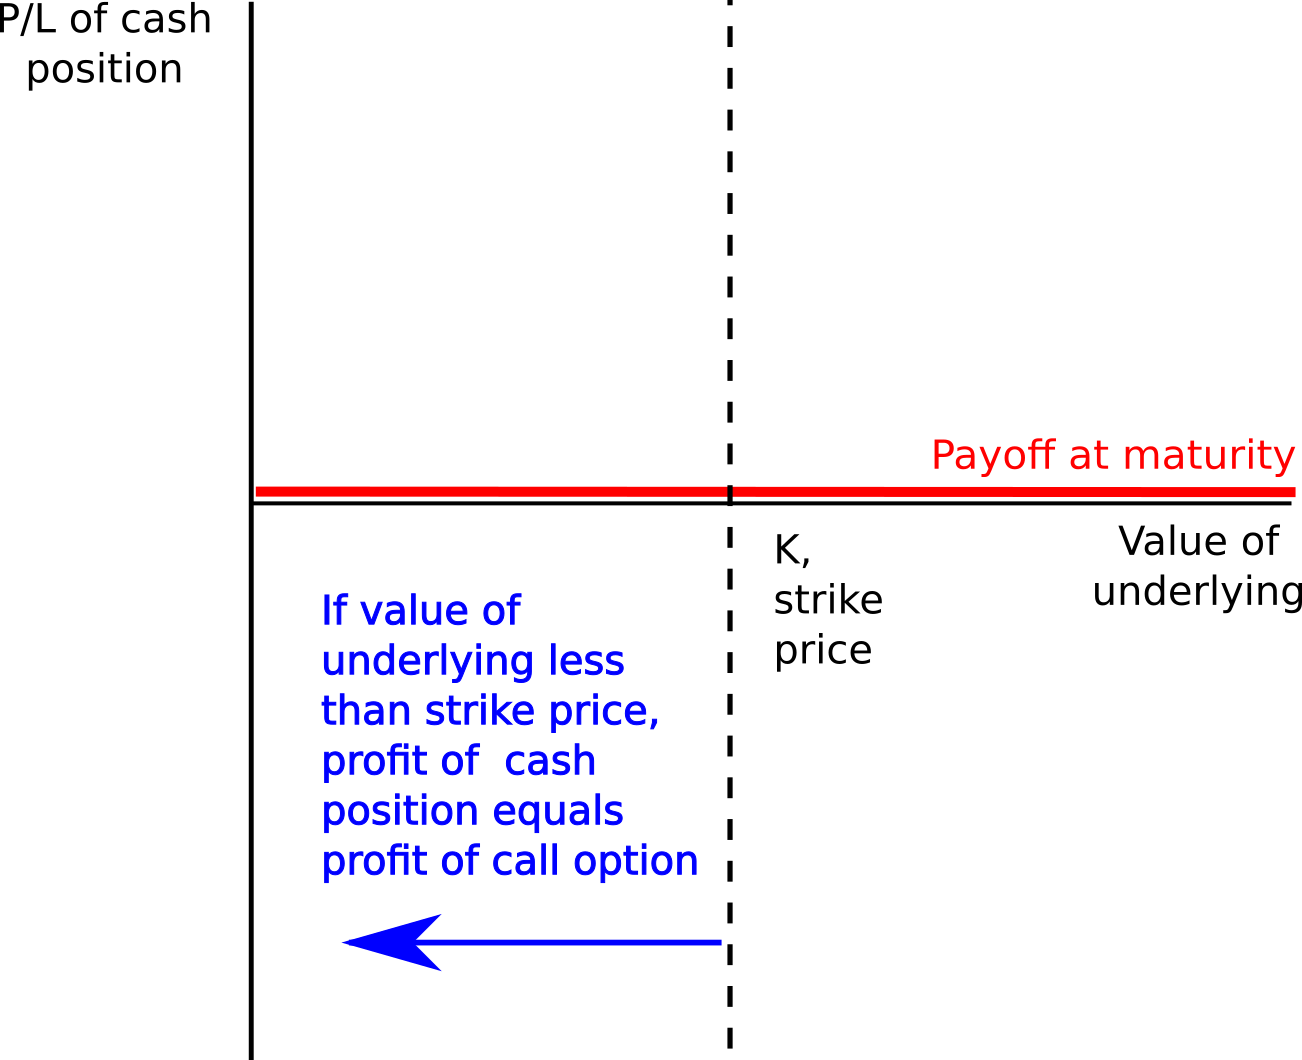
\includegraphics[width=0.6\linewidth]{images/figCashPosition} \caption{Payoff of a cash at maturity}\label{fig:unnamed-chunk-24}
\end{figure}

To replicate the option, we would hold a portfolio comprising some
amount of cash and some amount of a forward contract. Rather than using
the forward contract, we could replace it by using the underlying asset
itself. The spot exchange market is more liquid than the forward market.
Besides, referring to the mechanics of the synthetic USD loan, a forward
purchase itself could be replicated with a spot purchase and offsetting
domestic and foreign currency loans.

The share of each instrument in the portfolio changes constantly: the
more the option is ITM the closer its payoff resembles the payoff of the
forward contract. Hence, to replicate the option we would hold more
currency than cash. Viceversa, when the underlying declines and the
option shifts from being ITM to OTM, we will replace the currency
holdings with cash. \textbf{The option's \(\Delta\) determines the right
amount of currency needed to replicate the option}.

\begin{figure}
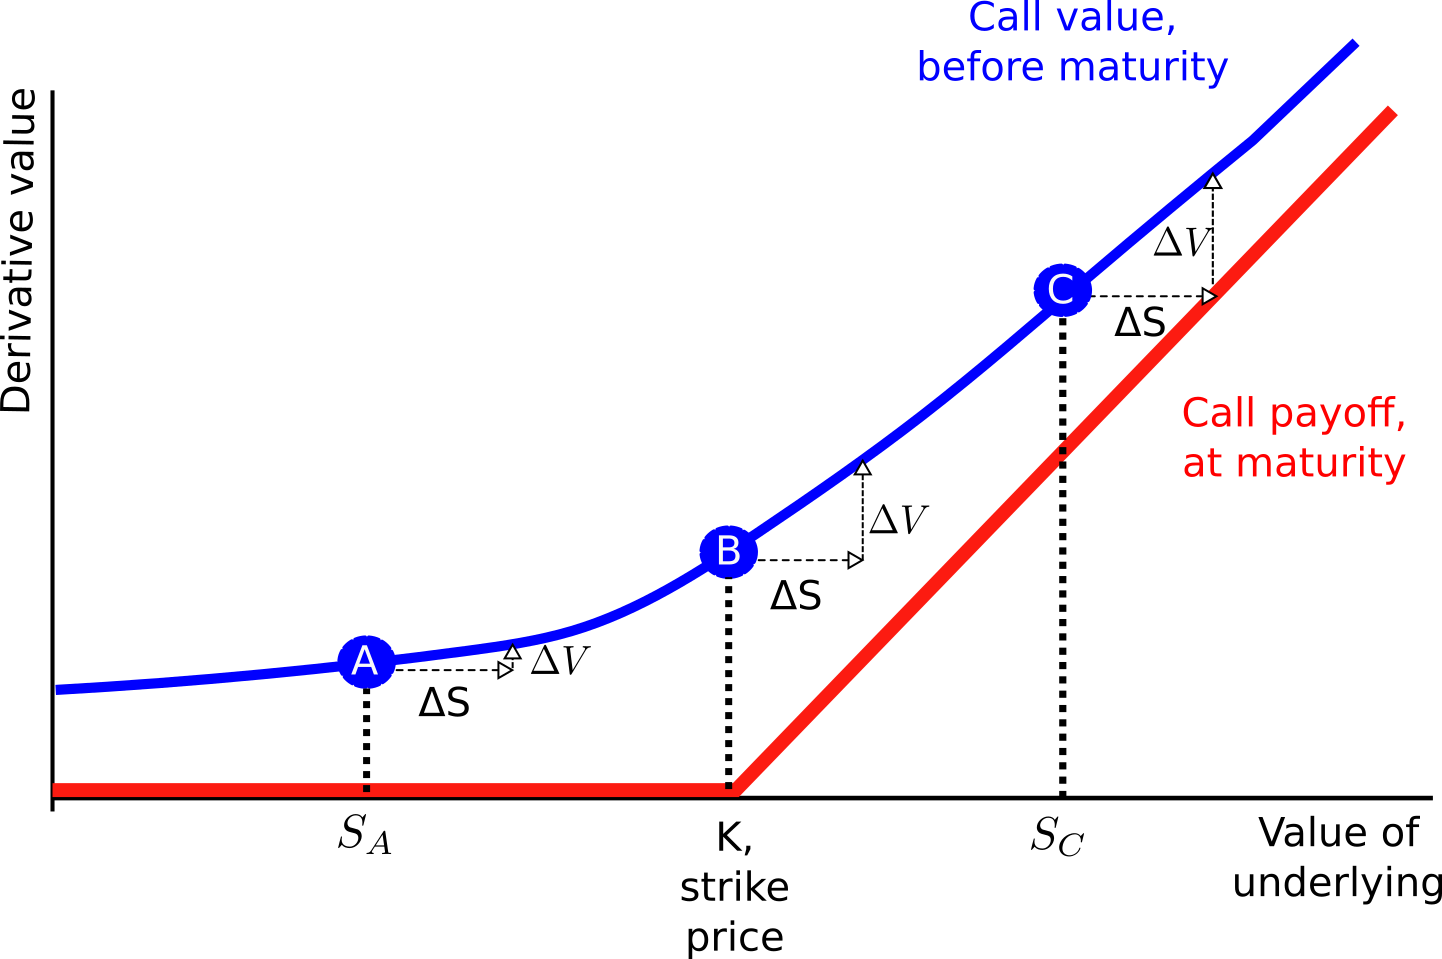
\includegraphics[width=0.7\linewidth]{images/figCallOption} \caption{$\Delta$ of call option before maturity}\label{fig:unnamed-chunk-25}
\end{figure}

Suppose we enter the option contract when the spot rate is equal to the
strike price (point \emph{B}). For each call option, we hold
\(\Delta_B\) units of the currency. Being the derivative of the call
option payoff, \(\Delta\) is always less or equal than one. If the
currency appreciates, the exchange rate moves to \(S_C\) (point
\emph{C}). The slope is steeper and \(\Delta_C > \Delta_B\). We have to
buy more currency to replicate the call. Conversely, if the currency
depreciates, we reduce our currency holdings since
\(\Delta_A < \Delta_B\).

\section{Pricing foreign currency
options}\label{pricing-foreign-currency-options}

Remember that dealers quote currency option prices in terms of vols, or
implied volatility. This parameter captures the costs involved in
replicating an option. Let's examine first what factors matter in the
replication process.

\subsection{Replicating the cost of a call
option}\label{replicating-the-cost-of-a-call-option}

The price of a currency option should reflect the costs the derivatives
dealer incurs to manufacture the option for the client and hedging the
associated risks. Take the case of a dealer buying a call option from a
client and holds it over a period of time \(\delta t\).

\begin{itemize}
\item
  The dealer first borrows the price of the call, \(C\), at the domestic
  interest rate \(R_d\). The funding cost is equal to: \[
  R_d C_t \delta t
  \]
\item
  The dealer's exposure is equivalent to a long position on the call. To
  neutralize it, it uses a dynamic replication to construct a short
  position on the call. As Box 1 explains, this requires selling
  \(\Delta\) units of the foreign currency. The proceeds from the sale,
  \(\Delta S\), can be reinvested at the domestic rate. Since the dealer
  borrows the foreign currency to sell it short, it has to pay the
  foreign currency interest rate, \(R_f\). This operation nets: \[
  (R_d - R_f) \Delta S_t  \delta t
  \]
\item
  During the period \(\delta t\), the option loses money. To understand
  why, assume you buy the option at maturity. You either pay nothing, if
  the option is OTM, or the difference between the spot exchange rate
  and the strike, if the option is ITM. If the option has not expired,
  even if it is OTM there is a chance that it could end up ITM at
  expiration time, and its value would be positive. The change in the
  value due to the passage of time is:
\end{itemize}

\[
\frac{\partial C_t}{\partial t} \delta t
\]

\begin{itemize}
\tightlist
\item
  The option has a non-linear payoff so it is necessary to add an
  additional term capturing what we refer to as ``convexity'' gains, as
  explained for instance in \citet{Neftci2008}. Mathematically, this
  adjustment is
\end{itemize}

\[
\frac{\partial^2 C_t}{\partial S^2} (\delta S_t)^2
\]

The change in the time value of the option plus the net gains from
hedging the long option position should offset the interest rate
payments completely:

\[
\frac{\partial C_t}{\partial t} \delta t + (R_d - R_f) \Delta S_t  \delta t + \frac{\partial^2 C}{\partial S_t^2} (\delta S_t)^2 = R_d C_t \delta t
\]

\subsection{The Garman-Kohlhagen
equation}\label{the-garman-kohlhagen-equation}

In the particular case of European options, and under the assumption
that the exchange rate follows a geometric Brownian motion, the equation
above simplifies to:

\[
\frac{\partial C_t}{\partial t} \delta t + (R_d - R_f) \Delta S_t  \delta t + \sigma^2 S^2\frac{\partial^2 C_t}{\partial S_t^2}\delta t  = R_d C_t \delta t
\]

After eliminating \(\delta t\), the solution of the equation yields the
formula for a call option at time \(t\) first derived by
\citet{Garman-Kohlhagen1983}:

\[
C(K,S_t,R_d,R_f,T,\sigma) = S_t \exp(-R_f\times(T-t))N(d_1) - K\exp(-R_d \times (T-t))N(d_2)
\]

where:

\begin{itemize}
\tightlist
\item
  \(K\) is the strike price,
\item
  \(S_t\) is the current spot exchange rate,
\item
  \(R_d\) is the domestic interest rate,
\item
  \(R_f\) is the foreign interest rate,
\item
  \(T-t\) is the remaining life of an option maturing at time \(T\),
\item
  \(\sigma\) is the implied volatility of the exchange rate used to
  price the option,
\end{itemize}

and:

\[
\begin{aligned}
d_1 &= \frac{\ln(S_t/K)+(R_d-R_f+\sigma^2/2)(T-t)}{\sigma \times (T-t)}\\
d_2 &= d_1 - \sigma \times (T-t)
\end{aligned}
\]

The price of a put option is:

\[
P(K,S_t,R_d,R_f,T,\sigma) = K\exp(-R_d \times (T-t))N(-d_2) - S_t \exp(-R_f\times(T-t))N(-d_1) 
\]

\section{Pricing conventions}\label{pricing-conventions}

We can map the value of almost all the variables in the pricing equation
to observed variables. The spot exchange rate is known, and the interest
rates correspond to the lending and borrowing rates, in domestic and
foreign currency, available to the derivatives dealers. The terms of the
contract must specify the maturity and the strike price of the option.
Add to this mix the implied volatility of the option, and the
Garman-Kohlhagen formula delivers the option price, or premium.

\subsection{\texorpdfstring{\(\Delta\)-implied
strikes}{\textbackslash{}Delta-implied strikes}}\label{delta-implied-strikes}

The market convention is to specify strike prices corresponding to a
given \(\Delta\). In such way, both parties are certain that the traded
option would have certain specific characteristics regardless of the
time it takes to agree on a price. Liquidity in currency options is
mainly concentrated in the \(ATM\) and 25\(\Delta\) strikes. For some
currency pairs, the 10\(\Delta\) strikes are also very liquid. To
recover the strike as an exchange rate, one reverse-engineers the
Garman-Kohlhagen formula using market reference benchmarks. For other
strike prices, the dealer interpolates prices obtained from a volatility
smile constructed using the price of the liquid \(ATM\), 25\(\Delta\),
and 10\(\Delta\) options.

\subsection{Implied volatility}\label{implied-volatility}

The price of the option is quoted as implied volatility, or vol, rather
than an actual money premium. To obtain the latter, the client has to
input the implied volatility and the \(\Delta\) implied strike in the
Garman-Kohlhagen formula. The other pricing inputs are set equal to
market reference benchmarks.

It is tempting to assume that implied volatility is either the
historical realized volatility or a forecast of realized volatility
during the life of the option. It is actually none of them. The value of
the implied volatility is such that the associated option premium
reflects a profit margin; the hedging costs of the dealer, which should
account for market frictions; and the demand and supply conditions in
the markets for the underlying and its derivatives instruments.

Hedging is imperfect due to several frictions. The credit quality of the
dealer and its counterparties affect the bid and ask rates for borrowing
and lending in the domestic and foreign currency.\footnote{See
  \citet{Lou2015}} Liquidity conditions also affect these rates,
especially for larger transactions. Finally, transaction costs prevent
continuous hedging leaving the dealer exposed at certain times. Exchange
rates can jump, as it was the case of the GBPUSD in June 2016. Hedging
jumps in the value of the underlying is extremely difficult, so some of
the potential losses should be passed to the client.

Although implied volatility does not necessarily reflect past or future
volatility, it prices supply and demand conditions driven partly by
market participants' positioning at certain exchange rate values and
ranges. This information, when interpreted within the volatility smile
framework, is useful for assessing exchange rate risks.

\chapter{The volatility smile}\label{the-volatility-smile}

Quoting implied vols for a selected range of \(\Delta\)s and maturities
has some advantages. First, it singles specific option contracts. For
instance, it is possible to monitor how the price of the constant
3-month maturity 25\(\Delta\) call option evolves over time. At any
time, the strike price is set such that \(\Delta\) is equal to 0.25. If
in contrast, we were monitoring a contract with a specific strike price
in terms of the value of the exchange rate, the contract \(\Delta\)
would be changing constantly as the spot rate and interest rates are
different.

Second, the fact that prices are quoted in volatility units facilitates
comparing prices at different points in time. Were the premium quoted in
money terms, i.e.~US dollar per British pound, it would be difficult to
state whether the option has become cheaper or more expensive since the
premium reflect the effect of several variables besides the implied
volatility parameter. But the latter is the one that captures the cost
of manufacturing the option, including demand and supply effects.

The main advantage of the market convention, however, is that it
identifies the three main unobserved drivers of currency option prices:
level, slope, and curvature.\footnote{These three factors are analogous
  to the level, slope, and curvature factors that completely
  characterize the behavior of the yield curve
  \citep{Litterman-Scheinkman1991}.} We analyze them using the \(ATM\)
vol, and the implied volatilities of the 25\(\Delta\) call, and the
75\(\Delta\) call. Dealers only quote the value of the first instrument.
But some simple algebra and an application of the put-call parity yields
the values of the last two instruments using the price quotes for the
risk reversals and butterfly spreads:

\[
\begin{aligned}
  \sigma_{25\Delta C} &= \sigma_{ATM} + BF_{25\Delta} + \frac{1}{2} RR_{25\Delta}\\
  \sigma_{25\Delta P} &= \sigma_{ATM} + BF_{25\Delta} - \frac{1}{2} RR_{25\Delta}\\
  \sigma_{75\Delta C} &= \sigma_{25\Delta P}
\end{aligned}
\]

With these three points, it is possible to fit a second-degree
polynomial, or a non-parametric spline function associating an implied
volatility to any \(\Delta\). This is the \textbf{volatility smile} in
the \(\Delta\)- volatility space, and we can use it to price options
with strikes other than the \(ATM\) and those implied by the
25\(\Delta\) and 75\(\Delta\).

\section*{Box 2. Put-call parity}\label{box-2.-put-call-parity}
\addcontentsline{toc}{section}{Box 2. Put-call parity}

The combination of a short put position (sell the put) and a long call
position (buy the call) mimics the payoff of a long forward position
(buy the currency forward) with strike price equal to the forward rate,
\(F\), at maturity:

\begin{figure}
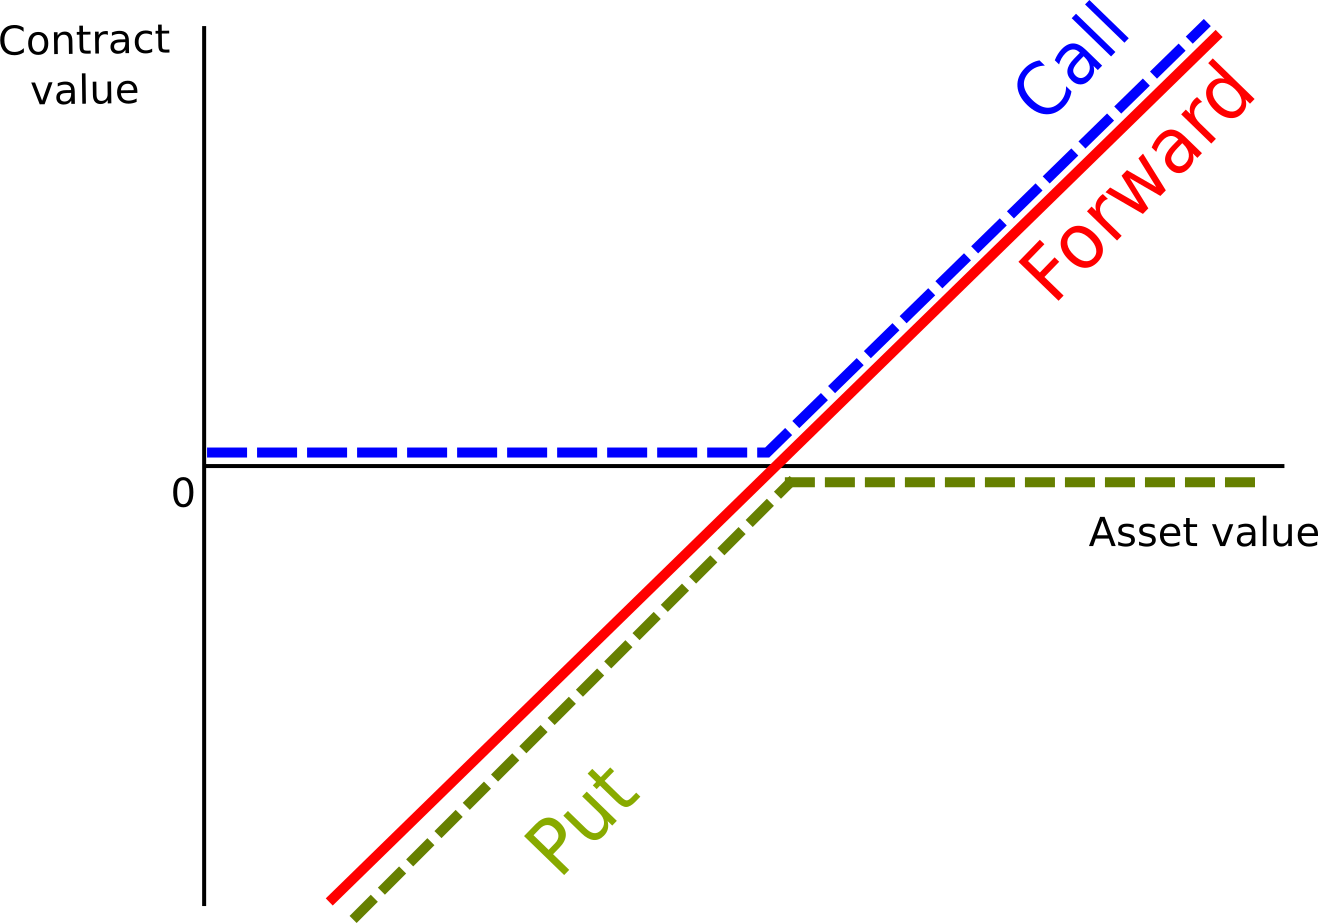
\includegraphics[width=0.6\linewidth]{images/figPutCallParity01} \caption{Put-call parity}\label{fig:unnamed-chunk-26}
\end{figure}

The following equality must hold:

\[
C(T) - P(T) = F(T)
\]

where \(C(T)\), \(P(T)\), and \(F(T)\) are prices of the call, the put,
and the forward at maturity, \(T\). If the contracts are entered at time
0, the present value of the option position, \(C(0) - P(0)\) should
still be the same as the present value of the forward position,
\(F \exp(-R_d \times T)\), where \(R_d\) is the domestic discount rate.
But the value of \(F\) is determined by the covered interest parity
conditions and equal to

\[
F= S(0) \exp((R_d-R_f) \times T ),
\]\\
where \(R_f\) is the foreign discount rate. The put-call parity follows:

\[
C(0) - P(0) = S(0) \exp(-R_f \times T)
\]

Taking derivatives with respect to \(S(0)\) yields the following
relationship between the \(\Delta\)s of a call and a put:

\[
\Delta_C - \Delta_P = \exp(-R_f \times T)
\]

When the foreign interest rate is small and/or the time to maturity is
short, the put-call parity is approximately ~ \[
\Delta_C - \Delta_P \approx 1
\]\\

\section{Level}\label{level}

To see the association between the \(ATM\) vol and the level effect,
Payne increased the \(ATM\), 25\(\Delta\), and 75\(\Delta\) vols by the
same amount, \(\delta\). She drew a chart showing the impact on the
volatility smile before and after the vol increase:

\begin{figure}
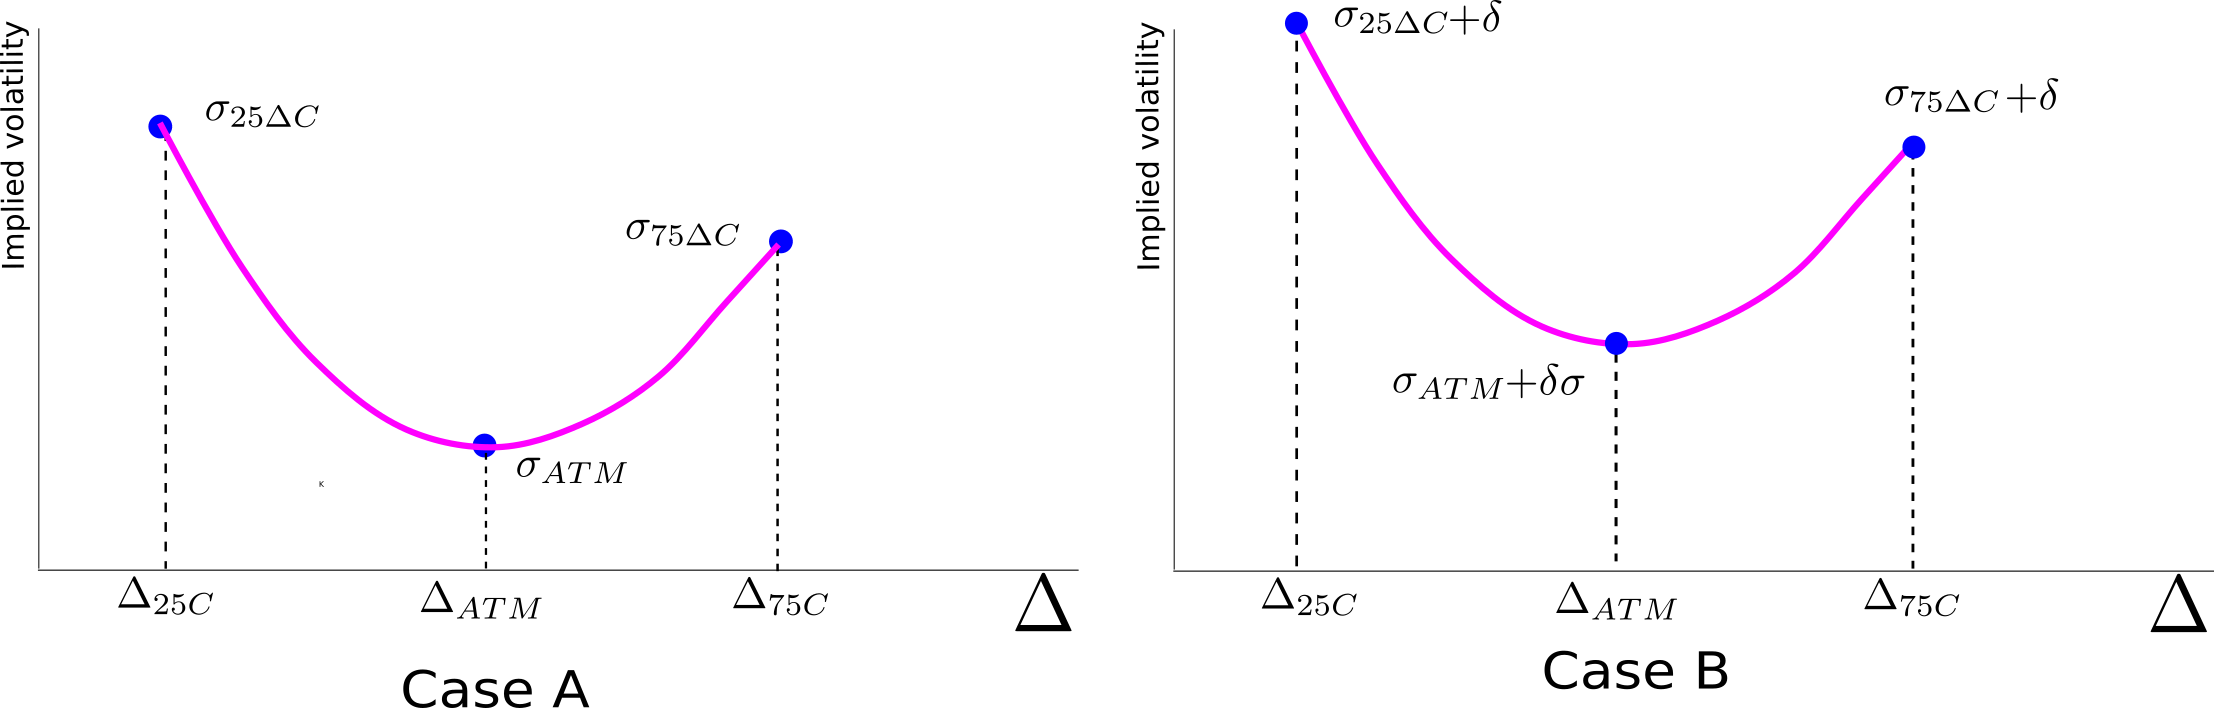
\includegraphics[width=1\linewidth]{images/figRRLevel} \caption{The $ATM$ vol reflects the level of the smile}\label{fig:unnamed-chunk-27}
\end{figure}

The shape of the volatility smile did not change at all. This was the
expected result: Payne remembered, from her high school algebra classes,
that such transformation was equivalent to just an upward translation of
the parabola determined by the three points. All things equal, changes
in \(\sigma_{ATM}\) only implies an upward or downward movements of the
volatility smile, clearly a level effect. Note that the butterfly spread
remains unchanged.

\section{Slope}\label{slope}

The other thought experiment Payne conducted was to change the values of
the wings in the original chart. Basically, she increased the vol of the
75\(\Delta\) call (or 25\(\Delta\) put) by \(\delta\), and reduced by
the same amount the vol of the 25\(\Delta\) call. The chart below
captured the results of the experiment:

\begin{figure}
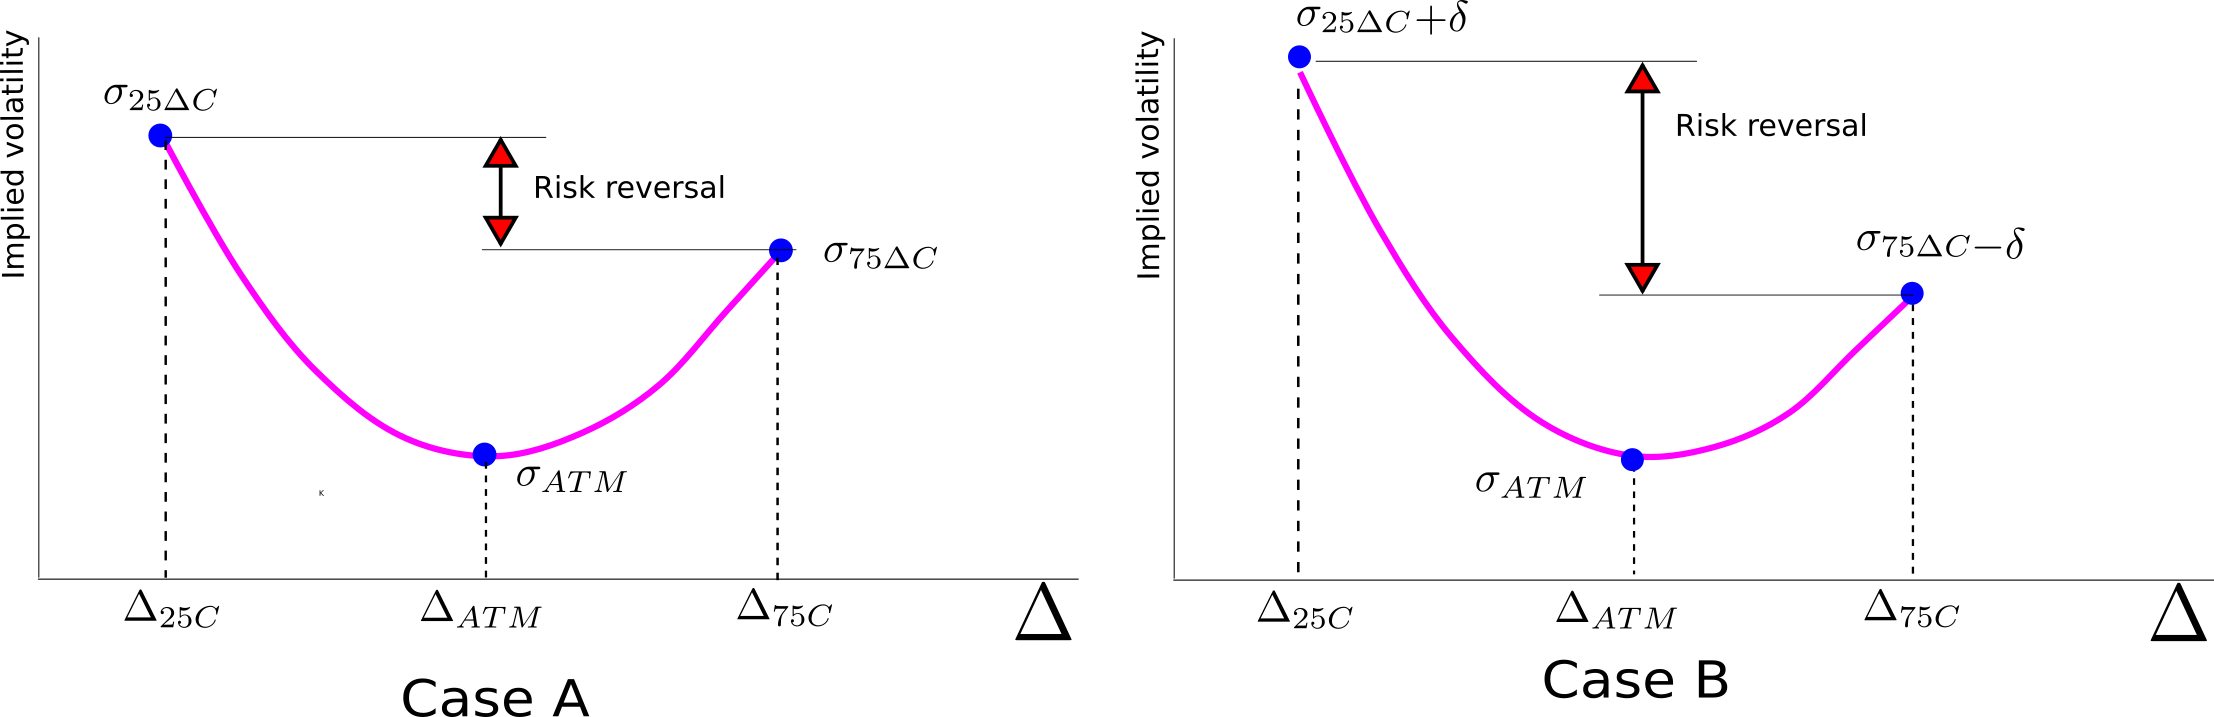
\includegraphics[width=1\linewidth]{images/figRRSlope} \caption{The risk-reversal reflects the slope of the smile}\label{fig:unnamed-chunk-28}
\end{figure}

The difference between the vols in the wings increased. In other words,
the absolute magnitude of the risk reversal,
\(|\sigma_{25\Delta C} - \sigma_{75\Delta C}|\), increased. If we were
to draw a line between the 25\(\Delta\) and the 75\(\Delta\), we would
notice a steepening of the slope of the line. The risk reversal was
clearly associated with the slope of the smile.

\section{Curvature}\label{curvature}

``Suppose the \(ATM\) vol remains unchanged but the volatility in the
wings decreases'' thought Payne. She did that and drew a chart similar
to the one below:

\begin{figure}
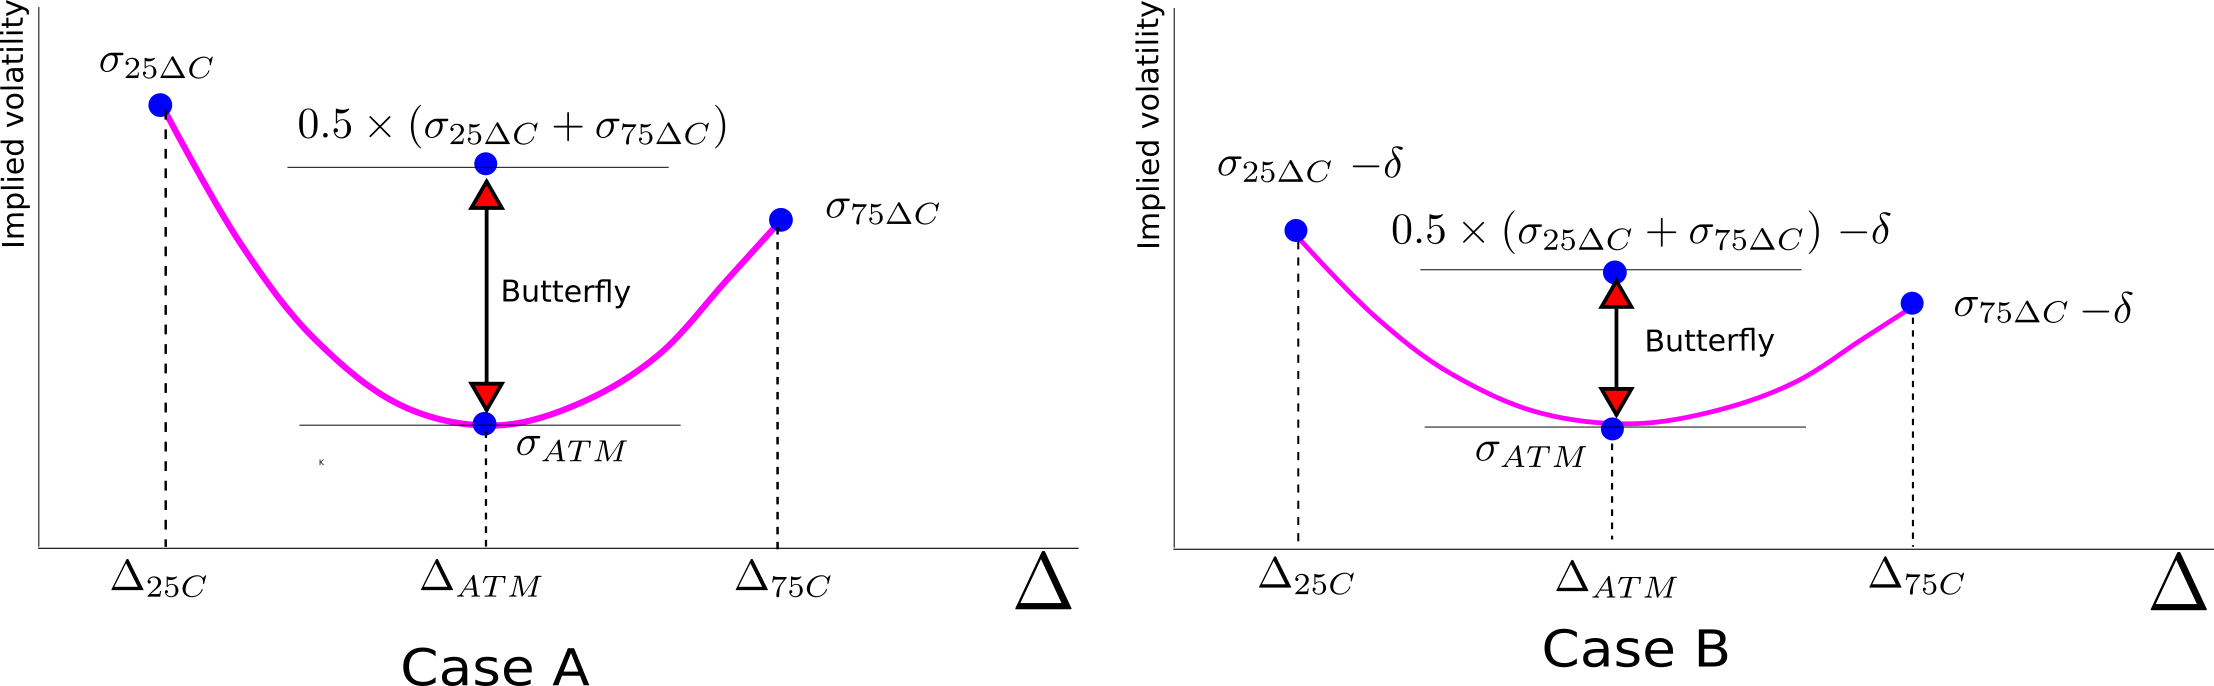
\includegraphics[width=1\linewidth]{images/figRRCurvature} \caption{The butterfly spread reflects the curvature of the smile}\label{fig:unnamed-chunk-29}
\end{figure}

Flat volatility smiles correspond to low values of the butterfly spread.
With three instruments capturing the level, slope, and curvature of the
volatility smile, it is possible to replicate a large range of shapes of
the volatility smile as long as they are either strictly convex or
concave.

\chapter{Constructing the smile}\label{constructing-the-smile}

Payne decided to focus her analysis on three specific dates (or
episodes):

\begin{itemize}
\tightlist
\item
  January 8, 2016 (Pre-Brexit)
\item
  June 24, 2016 (Brexit)
\item
  December 1, 2017 (Post-Brexit)
\end{itemize}

Roughly, the dates corresponded to six months ahead of the Brexit
referendum, the week of the referendum, and the six months after the
referendum.

In addition to the prices of the 25\(\Delta\) options, she needed the
prices of the 10\(\Delta\) options. The equations below, analogous to
the ones used to obtain the information from the 25\(\Delta\) options,
would prove handy for obtaining them:

\[
\begin{aligned}
  \sigma_{10\Delta C} &= \sigma_{ATM} + BF_{10\Delta} + \frac{1}{2} RR_{10\Delta}\\
  \sigma_{10\Delta P} &= \sigma_{ATM} + BF_{10\Delta} - \frac{1}{2} RR_{10\Delta}\\
  \sigma_{90\Delta C} &= \sigma_{10\Delta P}
\end{aligned}
\]

Before performing the calculations Payne had to select the appropriate
software. One option, which everybody at the IMF used, was Excel. One
advantage was that free files were available in any dark corner in the
IMF building. But there were horror stories about Excel: once one was
hooked on it, it was impossible to abandon it. Some of her colleagues
considered it even worse than being hooked on meth: users were saddled
with the mental suffering and distress but did not experience any highs
at all.

\texttt{Matlab} was the other available software she could use but it
was very expensive. The money was better spent buying a new Honda Accord
fully equipped. She decided to use \texttt{R}, a free software
environment for statistical computing and graphics, with many available
state-of-the-art libraries \citep{R-base}. Furthermore, the savings
could go into her defined-contribution retirement plan and allowed her
to take the 50 option if she so desired.

\section{Selecting the data for specific
dates}\label{selecting-the-data-for-specific-dates}

After begging the Internal Technocratic Diktat (ITD) Committee for
permission to install the non-white-listed software, Payne finally got
\texttt{R} and the \texttt{RStudio} IDE installed and running in her
laptop. To read the data for the specific dates of the analysis she
typed:

\begin{Shaded}
\begin{Highlighting}[]
\KeywordTok{rm}\NormalTok{(}\DataTypeTok{list=}\KeywordTok{ls}\NormalTok{())                                     }\CommentTok{# Clean up memory}
\NormalTok{filename =}\StringTok{ "2018_IET_Options_data.csv"}            \CommentTok{# Name of CSV data file}
\NormalTok{data =}\StringTok{ }\KeywordTok{read.csv}\NormalTok{(filename, }\DataTypeTok{header=}\OtherTok{TRUE}\NormalTok{)            }\CommentTok{# Load datafile}
\NormalTok{data}\OperatorTok{$}\NormalTok{Dates =}\StringTok{ }\KeywordTok{mdy_hm}\NormalTok{(}\KeywordTok{as.character}\NormalTok{(data}\OperatorTok{$}\NormalTok{Dates))     }\CommentTok{# convert dates to Date class}
\KeywordTok{rownames}\NormalTok{(data)=}\OtherTok{NULL}                               \CommentTok{# remove row names}

\CommentTok{# Specify dates for analysis}

\NormalTok{date01 =}\StringTok{ }\KeywordTok{as.Date}\NormalTok{(}\StringTok{"2016-01-08 UTC"}\NormalTok{)                 }
\NormalTok{date02 =}\StringTok{ }\KeywordTok{as.Date}\NormalTok{(}\StringTok{"2016-06-24 UTC"}\NormalTok{)}
\NormalTok{date03 =}\StringTok{ }\KeywordTok{as.Date}\NormalTok{(}\StringTok{"2017-12-01 UTC"}\NormalTok{)}

\CommentTok{# Create data frame this.data}

\NormalTok{this.data =}\StringTok{ }\KeywordTok{rbind}\NormalTok{(}
\NormalTok{  data[}\KeywordTok{which}\NormalTok{(data}\OperatorTok{$}\NormalTok{Dates}\OperatorTok{==}\NormalTok{date01),],}
\NormalTok{  data[}\KeywordTok{which}\NormalTok{(data}\OperatorTok{$}\NormalTok{Dates}\OperatorTok{==}\NormalTok{date02),],}
\NormalTok{  data[}\KeywordTok{which}\NormalTok{(data}\OperatorTok{$}\NormalTok{Dates}\OperatorTok{==}\NormalTok{date03),])}

\CommentTok{# Delete row names and change the names of the columns}

\KeywordTok{rownames}\NormalTok{(this.data) =}\StringTok{ }\OtherTok{NULL}
\KeywordTok{colnames}\NormalTok{(this.data) =}\StringTok{ }\KeywordTok{c}\NormalTok{(}\StringTok{"Date"}\NormalTok{,}\StringTok{"spot"}\NormalTok{,}\StringTok{"forward"}\NormalTok{,}\StringTok{"atm"}\NormalTok{, }\StringTok{"rr25"}\NormalTok{,}\StringTok{"bf25"}\NormalTok{,}
                        \StringTok{"rr10"}\NormalTok{,}\StringTok{"bf10"}\NormalTok{,}\StringTok{"rf"}\NormalTok{,}\StringTok{"rd"}\NormalTok{,}\StringTok{"imp_rd"}\NormalTok{)}
\end{Highlighting}
\end{Shaded}

\section{Calculation of implied volatilities
(vols)}\label{calculation-of-implied-volatilities-vols}

The following lines of code used the information from the risk reversals
and the butterfly spreads to calculate the vols of the different calls
and puts:

\begin{Shaded}
\begin{Highlighting}[]
\CommentTok{# Vols are in percent, expressed them as simple numbers}
\NormalTok{this.data}\OperatorTok{$}\NormalTok{atm  =}\StringTok{ }\NormalTok{this.data}\OperatorTok{$}\NormalTok{atm}\OperatorTok{/}\DecValTok{100}
\NormalTok{this.data}\OperatorTok{$}\NormalTok{rr25 =}\StringTok{ }\NormalTok{this.data}\OperatorTok{$}\NormalTok{rr25}\OperatorTok{/}\DecValTok{100}
\NormalTok{this.data}\OperatorTok{$}\NormalTok{bf25 =}\StringTok{ }\NormalTok{this.data}\OperatorTok{$}\NormalTok{bf25}\OperatorTok{/}\DecValTok{100}
\NormalTok{this.data}\OperatorTok{$}\NormalTok{rr10 =}\StringTok{ }\NormalTok{this.data}\OperatorTok{$}\NormalTok{rr10}\OperatorTok{/}\DecValTok{100}
\NormalTok{this.data}\OperatorTok{$}\NormalTok{bf10 =}\StringTok{ }\NormalTok{this.data}\OperatorTok{$}\NormalTok{bf10}\OperatorTok{/}\DecValTok{100}
\NormalTok{this.data}\OperatorTok{$}\NormalTok{rf   =}\StringTok{ }\NormalTok{this.data}\OperatorTok{$}\NormalTok{rf}\OperatorTok{/}\DecValTok{100}
\NormalTok{this.data}\OperatorTok{$}\NormalTok{rd   =}\StringTok{ }\NormalTok{this.data}\OperatorTok{$}\NormalTok{rd}\OperatorTok{/}\DecValTok{100}
\NormalTok{this.data}\OperatorTok{$}\NormalTok{imp_rd=this.data}\OperatorTok{$}\NormalTok{imp_rd}\OperatorTok{/}\DecValTok{100}

\CommentTok{# We will use this.data repeatedly}
\CommentTok{# Attach it to access its elements}

\KeywordTok{attach}\NormalTok{(this.data)     }

\CommentTok{# Recover vols for different deltas and put them in the data frame}

\NormalTok{this.data}\OperatorTok{$}\NormalTok{sigma10c =}\StringTok{ }\NormalTok{atm }\OperatorTok{+}\StringTok{ }\NormalTok{bf10 }\OperatorTok{+}\StringTok{ }\FloatTok{0.5}\OperatorTok{*}\NormalTok{rr10}
\NormalTok{this.data}\OperatorTok{$}\NormalTok{sigma25c =}\StringTok{ }\NormalTok{atm }\OperatorTok{+}\StringTok{ }\NormalTok{bf25 }\OperatorTok{+}\StringTok{ }\FloatTok{0.5}\OperatorTok{*}\NormalTok{rr25}
\NormalTok{this.data}\OperatorTok{$}\NormalTok{sigma75c =}\StringTok{ }\NormalTok{this.data}\OperatorTok{$}\NormalTok{sigma25c }\OperatorTok{-}\StringTok{ }\NormalTok{rr25}
\NormalTok{this.data}\OperatorTok{$}\NormalTok{sigma90c =}\StringTok{ }\NormalTok{this.data}\OperatorTok{$}\NormalTok{sigma10c }\OperatorTok{-}\StringTok{ }\NormalTok{rr10}
\NormalTok{this.data}\OperatorTok{$}\NormalTok{sigmaatm =}\StringTok{ }\NormalTok{atm}

\NormalTok{Tenor =}\StringTok{ }\DecValTok{3}\OperatorTok{/}\DecValTok{12}   \CommentTok{# Maturity of options, 3 months, in years}
\end{Highlighting}
\end{Shaded}

The tenor, or time to maturity of the option, was set to
\(\frac{3}{12} = 0.25\) years, to be consistent with the market
convention for implied volatility, which is annualized.

\section{\texorpdfstring{\(\Delta_{ATM}\) market
convention}{\textbackslash{}Delta\_\{ATM\} market convention}}\label{delta_atm-market-convention}

So far, the only missing piece of information is the \(\Delta_{ATM}\),
or the \(\Delta\) associated with the \(ATM\) option. ``How do I
calculate that number?'' Payne wondered aloud. As the reader can guess,
the definition of the \(ATM\) option depends on what convention the
market uses. There are three different conventions:

\begin{itemize}
\item
  for retail products, the \(ATM\) strike is the current spot rate. In
  this case:\\
  \[
  \begin{aligned}
  K_{ATM} &= S\\
  \Delta_{ATM} &= N \left(\frac{\log(F/S) + \frac{1}{2} \sigma_{ATM}^2 T}{\sigma_{ATM} \sqrt T} \right)
  \end{aligned}
  \]
\item
  for emerging market currencies and/or options with maturities above
  one year, the \(ATM\) strike is the forward rate, or the \(ATMF\). In
  this case: \[
  \begin{aligned}
  K_{ATM} &= F\\
  \Delta_{ATM} &= \exp(-Rf \times T)N(\frac{1}{2}\sigma_{ATM} \sqrt T) 
  \end{aligned}
  \]
\item
  for major currency pair and/or options with maturities of one year or
  less, the \(ATM\) strike is the value of the exchange rate such that
  the call and the put have the same \(\Delta\). In this case,
  \(\Delta_{ATM} \simeq 0.5\) and the strike price \(K_{ATM}\) is:\\
  \[
  \begin{aligned}
   K_{ATM} &= F \times \exp\left( 0.5 \sigma^2_{ATM}\times T \right)\\
   \Delta_{ATM} &= 0.5\times exp(-Rf \times T) \simeq 0.5 
  \end{aligned}
  \]
\end{itemize}

The pair GBP-USD required using the third market convention. Payne
calculated the strike of the \(ATM\) option and its \(\Delta\):

\begin{Shaded}
\begin{Highlighting}[]
\CommentTok{# Calculate the strike of the ATM option}
\NormalTok{K_atm =}\StringTok{ }\NormalTok{forward}\OperatorTok{*}\KeywordTok{exp}\NormalTok{((}\FloatTok{0.5}\OperatorTok{*}\NormalTok{(this.data}\OperatorTok{$}\NormalTok{sigmaatm)}\OperatorTok{^}\DecValTok{2}\NormalTok{)}\OperatorTok{*}\NormalTok{Tenor)}
\NormalTok{deltaATM =}\StringTok{ }\FloatTok{0.5}\OperatorTok{*}\KeywordTok{exp}\NormalTok{(}\OperatorTok{-}\NormalTok{rf}\OperatorTok{*}\NormalTok{Tenor)}
\end{Highlighting}
\end{Shaded}

\section{A rough first pass on the volatility
smile}\label{a-rough-first-pass-on-the-volatility-smile}

In the case of the GBPUSD, the \(\Delta_{ATM}\) could be very well
approximated by \(0.5\). To check the data, Payne decided to plot of the
volatility smile. First, she created the data frame with the information
the plot required:

\begin{Shaded}
\begin{Highlighting}[]
\CommentTok{# Select only the vols for each delta}
\NormalTok{list_variables =}\StringTok{ }\KeywordTok{c}\NormalTok{(}\StringTok{"sigma10c"}\NormalTok{, }\StringTok{"sigma25c"}\NormalTok{, }\StringTok{"sigmaatm"}\NormalTok{, }\StringTok{"sigma75c"}\NormalTok{, }\StringTok{"sigma90c"}\NormalTok{)}

\CommentTok{# Read the data as a matrix}
\NormalTok{vol_data =}\StringTok{ }\KeywordTok{t}\NormalTok{(}\KeywordTok{as.matrix}\NormalTok{(}\KeywordTok{subset}\NormalTok{(this.data, }\DataTypeTok{select=}\NormalTok{list_variables)))}

\CommentTok{# Group the deltas in a vector, to be used in the x-axis}
\NormalTok{delta_vector =}\StringTok{ }\KeywordTok{c}\NormalTok{(}\FloatTok{0.10}\NormalTok{, }\FloatTok{0.25}\NormalTok{, }\FloatTok{0.5}\NormalTok{, }\FloatTok{0.75}\NormalTok{, }\FloatTok{0.9}\NormalTok{)}

\CommentTok{# Create the data frame for the chart}
\NormalTok{vol.smile  =}\StringTok{ }\KeywordTok{data.frame}\NormalTok{(delta_vector, vol_data)   }
\KeywordTok{rownames}\NormalTok{(vol.smile) =}\StringTok{ }\OtherTok{NULL}
\KeywordTok{colnames}\NormalTok{(vol.smile) =}\StringTok{ }\KeywordTok{c}\NormalTok{(}\StringTok{"Delta"}\NormalTok{,}\StringTok{"PreBrexit"}\NormalTok{,}\StringTok{"Brexit"}\NormalTok{,}\StringTok{"PostBrexit"}\NormalTok{)}
\end{Highlighting}
\end{Shaded}

and used \texttt{ggplot} to create the chart:

\begin{Shaded}
\begin{Highlighting}[]
\KeywordTok{library}\NormalTok{(reshape2)}
\NormalTok{vol.data =}\StringTok{ }\KeywordTok{melt}\NormalTok{(vol.smile, }\DataTypeTok{id=}\StringTok{"Delta"}\NormalTok{)}
\KeywordTok{ggplot}\NormalTok{(}\DataTypeTok{data=}\NormalTok{vol.data, }\KeywordTok{aes}\NormalTok{(}\DataTypeTok{x=}\NormalTok{Delta, }\DataTypeTok{y=}\NormalTok{value, }\DataTypeTok{shape=}\NormalTok{variable)) }\OperatorTok{+}
\StringTok{   }\KeywordTok{geom_point}\NormalTok{(}\KeywordTok{aes}\NormalTok{(}\DataTypeTok{colour=}\NormalTok{variable), }\DataTypeTok{size=}\DecValTok{4}\NormalTok{) }\OperatorTok{+}
\StringTok{   }\KeywordTok{labs}\NormalTok{(}\DataTypeTok{y=}\StringTok{"vol"}\NormalTok{)}
\end{Highlighting}
\end{Shaded}

\begin{figure}
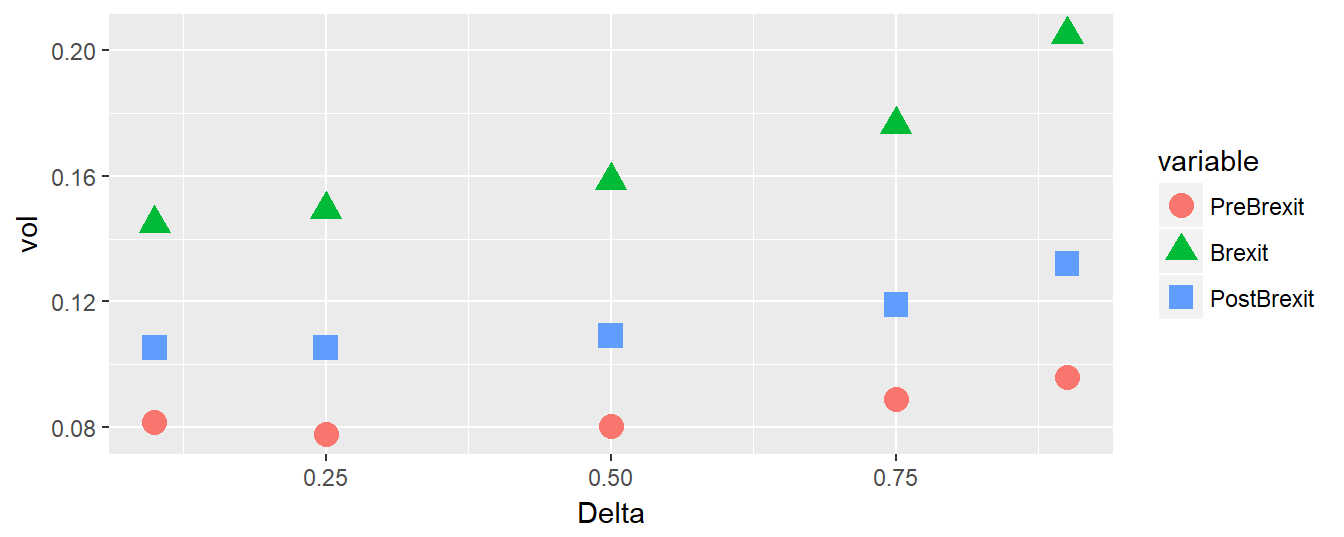
\includegraphics[width=1\linewidth]{images/unnamed-chunk-34-1} \caption{Rough volatility smiles}\label{fig:unnamed-chunk-34}
\end{figure}

\section{A more refined approximation of the volatility
smile}\label{a-more-refined-approximation-of-the-volatility-smile}

It is possible to extend the volatility smile over a wider range of
\(\Delta\) values using a polynomial approximation of second degree. The
function \texttt{fit.Vol()} in the \texttt{auxFile.R} takes as input the
observed vols and their corresponding \(\Delta\)s, and interpolates and
extrapolates the vols for a wider range of \(\Delta\) values:

\begin{Shaded}
\begin{Highlighting}[]
\CommentTok{# Function fit.vol fits a polynomial of second degree to the volatility smile}
\NormalTok{fit.Vol =}\StringTok{ }\ControlFlowTok{function}\NormalTok{(data.vol, data.delta,delta.range)}
\NormalTok{\{}
\NormalTok{  poly.fit =}\StringTok{ }\KeywordTok{lm}\NormalTok{(data.vol }\OperatorTok{~}\StringTok{ }\KeywordTok{poly}\NormalTok{(data.delta, }\DecValTok{2}\NormalTok{, }\DataTypeTok{raw=}\OtherTok{TRUE}\NormalTok{))  }

  \CommentTok{# Use fitted polynomial to interpolate Delta-Vol Curve}
\NormalTok{  delta.square =}\StringTok{ }\NormalTok{delta.range}\OperatorTok{*}\NormalTok{delta.range}
\NormalTok{  delta.interc =}\StringTok{ }\KeywordTok{rep}\NormalTok{(}\DecValTok{1}\NormalTok{,}\KeywordTok{length}\NormalTok{(delta.range))}
  
\NormalTok{  X =}\StringTok{ }\KeywordTok{cbind}\NormalTok{(delta.interc, delta.range, delta.square)}
\NormalTok{  iVolInterpol =}\StringTok{ }\KeywordTok{t}\NormalTok{(}\KeywordTok{t}\NormalTok{(X)}\OperatorTok{*}\NormalTok{poly.fit}\OperatorTok{$}\NormalTok{coefficients)}
\NormalTok{  iVolInterpol =}\StringTok{ }\KeywordTok{rowSums}\NormalTok{(iVolInterpol)}

  \KeywordTok{return}\NormalTok{(iVolInterpol)}
\NormalTok{\}}
\end{Highlighting}
\end{Shaded}

Payne used the \texttt{fitVol()} function to fit the volatility smile
for the pre-Brexit, Brexit, and post-Brexit dates:

\begin{Shaded}
\begin{Highlighting}[]
\CommentTok{# Get the data points from the vol.smile data frame}
\NormalTok{data.delta =}\StringTok{ }\NormalTok{vol.smile}\OperatorTok{$}\NormalTok{Delta}
\NormalTok{data.vol  =}\StringTok{ }\NormalTok{vol.smile}\OperatorTok{$}\NormalTok{PreBrexit}

\CommentTok{# Interpolation and extrapolation range}
\NormalTok{delta.range =}\StringTok{ }\KeywordTok{seq}\NormalTok{(}\DataTypeTok{from=}\FloatTok{0.01}\NormalTok{, }\DataTypeTok{to =} \FloatTok{0.99}\NormalTok{, }\DataTypeTok{by=}\FloatTok{0.005}\NormalTok{)}

\CommentTok{# Obtain the volatility smiles}
\NormalTok{smile.preBrexit =}\StringTok{ }\KeywordTok{fit.Vol}\NormalTok{(vol.smile}\OperatorTok{$}\NormalTok{PreBrexit, data.delta, delta.range)}
\NormalTok{smile.Brexit    =}\StringTok{ }\KeywordTok{fit.Vol}\NormalTok{(vol.smile}\OperatorTok{$}\NormalTok{Brexit, data.delta, delta.range)}
\NormalTok{smile.postBrexit =}\StringTok{ }\KeywordTok{fit.Vol}\NormalTok{(vol.smile}\OperatorTok{$}\NormalTok{PostBrexit, data.delta, delta.range)}

\CommentTok{# Group the extended volatility smiles in a data frame}
\NormalTok{smile.df =}\StringTok{ }\KeywordTok{data.frame}\NormalTok{(delta.range, smile.preBrexit, smile.Brexit, smile.postBrexit)}
\KeywordTok{rownames}\NormalTok{(smile.df) =}\StringTok{ }\OtherTok{NULL}
\KeywordTok{colnames}\NormalTok{(smile.df) =}\StringTok{ }\KeywordTok{c}\NormalTok{(}\StringTok{"Delta"}\NormalTok{,}\StringTok{"preBrexit"}\NormalTok{,}\StringTok{"Brexit"}\NormalTok{, }\StringTok{"postBrexit"}\NormalTok{)}

\CommentTok{# Create the chart}
\KeywordTok{library}\NormalTok{(reshape2)}
\NormalTok{smile.data =}\StringTok{ }\KeywordTok{melt}\NormalTok{(smile.df, }\DataTypeTok{id=}\StringTok{"Delta"}\NormalTok{)}
\KeywordTok{ggplot}\NormalTok{(}\DataTypeTok{data =}\NormalTok{ smile.data, }\KeywordTok{aes}\NormalTok{(}\DataTypeTok{x=}\NormalTok{Delta, }\DataTypeTok{y=}\NormalTok{value, }\DataTypeTok{colour=}\NormalTok{variable)) }\OperatorTok{+}\StringTok{ }\KeywordTok{geom_line}\NormalTok{(}\DataTypeTok{size=}\DecValTok{1}\NormalTok{) }\OperatorTok{+}
\StringTok{  }\KeywordTok{labs}\NormalTok{(}\DataTypeTok{y=}\StringTok{"vol"}\NormalTok{)}
\end{Highlighting}
\end{Shaded}

\begin{figure}
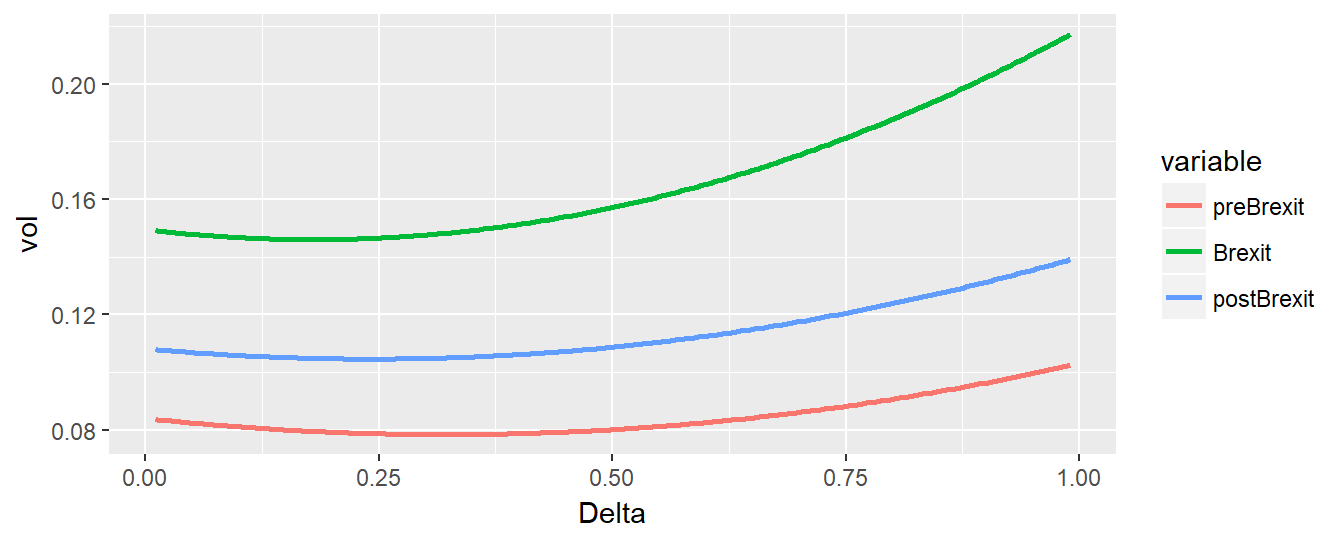
\includegraphics[width=1\linewidth]{images/unnamed-chunk-36-1} \caption{Fitted volatility smiles}\label{fig:unnamed-chunk-36}
\end{figure}

Before going further in her analysis, Payne asked herself a question:

Question: In the week of the Brexit referendum, does it make sense that
higher \(\Delta\)s have higher implied volatility values?

\chapter{Extracting the risk-neutral
density}\label{extracting-the-risk-neutral-density}

``Why am I estimating volatility smiles?'' Payne asked herself. But it
was a rhetorical question since she knew the answer.

The information contained in the volatility smile reflects the market
view on the future probability distribution of the exchange rate at the
time the option matures. But this market view is a risk-neutral view,
i.e., in most cases, it does not reflect the future movements of the
exchange rate. The next box offers an economic interpretation of risk
neutrality abstracting from mathematical arguments.\footnote{See
  \citet{Hull2017}, \citet{Cox-Ross-Rubinstein1979}, and
  \citet{Wilmott2006} for an accessible mathematical treatment.}

\section*{Box 3. Why market views are risk-neutral and different from
forecasts}\label{box-3.-why-market-views-are-risk-neutral-and-different-from-forecasts}
\addcontentsline{toc}{section}{Box 3. Why market views are risk-neutral
and different from forecasts}

The market view is a \textbf{risk-neutral} view. In other words, it is
not a forecast of the \textbf{objective} or real-world probability
distribution.\footnote{See, for instance,
  \citet{Constantinides-Jackwerth-Perrakis2007} and
  \citet{Garcia-Ghysels-Renault2009}.} Rather, it is a view distilled
from option prices that weigh the risk aversion of the different
participants in the derivatives market: hedgers, speculators, and market
makers. One example textbooks use is home insurance. Suppose the
insurance premium you pay increases. Does it imply that your house is
more likely to be damaged by a covered insurance event, i.e.~fire,
storm, etc? Not necessarily.

A better example, in the context of exchange rates, is the demand for
put options, or protection against a depreciation of the currency. This
might be a low probability event. Assume a scenario in which clients are
now more exposed to a depreciation. For instance, a substantial number
of corporations replace foreign currency debt for domestic currency debt
as foreign interest rates are low.

Hedging operations increase the demand for puts, driving the vols of the
puts up and leading to steeper risk reversals. Most of the hedging
demand would be satisfied with OTM puts. Derivatives dealers, with short
positions in these puts, need to ask for an additional premium. This
premium compensates them for a potential increase in their hedging costs
were the currency to depreciate. A depreciation will cause the OTM
options to become ITM, with a shorter time to maturity, which translates
into higher \(\Delta\) hedging costs.

In the scenario above, market participants' expectations about real
world exchange rate movements remain unchanged. But the skew of the
volatility smile, as captured by the risk reversal, has increased.

Furthermore, it is not easy to disentangle the risk aversion component
from the expectations component. It may well be the case that actually
the rising demand for puts reflects increased expectations of a
depreciation and not increased exposure to foreign currency liabilities.
As in the previous scenario, the skew of the volatility smile would
increase for the same reasons. And we could also have a hybrid case,
where both exchange rate expectations and increased exposure drive the
demand for puts higher.

As the box makes clear, the best interpretation of the risk-neutral
distribution is as a risk-aversion weighted probability distribution. It
shows whether the \textbf{\emph{market fears certain events more than
others}}, and whether this fear is increasing or subsiding in time.
Although the risk-neutral distribution may not be a good forecast of
exchange rate movements, it highlights events that are of concern to
market participants. This information could guide both market strategy,
and policy decisions as well, as they could point to potential sources
of financial instability.\footnote{\href{https://www.minneapolisfed.org/banking/mpd/resources/papers/market-based-probabilities-a-tool-for-policymakers}{Federal
  Reserve Bank of Minneapolis, Market based probabilities: a tool for
  policy makers.}}

\section{Extraction techniques}\label{extraction-techniques}

Most of the extraction techniques, and arguably the most useful ones,
are non-structural, i.e.~they do not need to specify a model for the
dynamics of the price of the underlying asset, or the exchange rate in
this case. Non-structural techniques fall under one of two different
categories:\footnote{See \citet{Mandler2003} and \citet{Jackwerth2004}.}

\begin{itemize}
\tightlist
\item
  Parametric methods.
\item
  Semiparametric methods
\item
  Non-parametric methods.
\end{itemize}

Parametric methods typically specify a distribution function for the
exchange rate at the maturity time. Given a distribution \(F\), the
price of an option with a strike price \(K\) is simply the present value
of the expected payoff of the option. For a call option, with maturity
and time to expiration \(T\), its present value is:

\[
C^F(K) = \exp(-R_d\times T) \int_{K}^{\infty} \left( S_T - K\right) dF(S_T; \Lambda), 
\]

where \(F\) is a distribution function with parameters \(\Lambda\). The
best approximation to the market-implied distribution corresponds to the
parameters that satisfy:

\[
\arg\min_{\Lambda} \sum_{j=1}^N |C^F(K_j) - C^{\text{Market}}(K_j)|^2
\]

One widely used parametric method relies on the generalized beta
distribution, which we will implement in a later section
\citep{Bookstaber-McDonald1987}.

Semiparametric methods start with a particular density, i.e.~the
log-normal density or the Gaussian density, and add expansion terms in
order to fit the observed market prices of the options, as in
\citet{Jarrow-Rudd1982}.

Non-parametric methods rely on the observation that the shape of the
\textbf{market call function,} a plot of the value of the call against
different strike prices, contains useful information about the
probability distribution of the underlying. Specifically,
\citet{Breeden-Litzenberger1978} showed that the risk-neutral
probability density, \(q\), is proportional to the second derivative of
the call premium with respect to the strike price:

\[
\frac{\partial^2 C}{\partial K^2} \bigg\rvert_{K=S} = \exp(-R_d \times T)q(S).
\]

The next section explains how Payne implemented some of these methods.

\section{Infering premia and strike prices from
vols}\label{infering-premia-and-strike-prices-from-vols}

Non-structural methods require data on option prices for different
strikes, or inferring the premium-strike price function from the
volatility smile.

Recall that the volatility smile data shows the price, in vols, of
options with different \(\Delta\). The \texttt{auxFile.R} contains the
function \texttt{get.strike()}, which Payne used to find the strike
prices corresponding to each \(\Delta\) value:

\begin{Shaded}
\begin{Highlighting}[]
\NormalTok{get.strike =}\StringTok{ }\ControlFlowTok{function}\NormalTok{(vol,delta,S0,fwd,rf,Tenor)}
\CommentTok{# Inputs}
\CommentTok{#   vol:     implied volatility}
\CommentTok{#   S0 :     spot exchange rate}
\CommentTok{#   fwd:     forward exchange rate}
\CommentTok{#   rf:      foreign currency interest rate}
\CommentTok{#   Tenor:   time to maturity of the option}
\CommentTok{#}
\CommentTok{# Note: since we use the forward rate, the domestic}
\CommentTok{#       interest rate is not needed}
\NormalTok{\{}
\NormalTok{  aux =}\StringTok{ }\KeywordTok{qnorm}\NormalTok{(delta}\OperatorTok{*}\KeywordTok{exp}\NormalTok{(rf}\OperatorTok{*}\NormalTok{Tenor))}
\NormalTok{  aux =}\StringTok{ }\NormalTok{aux}\OperatorTok{*}\NormalTok{vol}\OperatorTok{*}\KeywordTok{sqrt}\NormalTok{(Tenor)}
\NormalTok{  aux =}\StringTok{ }\NormalTok{aux }\OperatorTok{-}\StringTok{ }\FloatTok{0.5}\OperatorTok{*}\NormalTok{vol}\OperatorTok{*}\NormalTok{vol}\OperatorTok{*}\NormalTok{Tenor}
\NormalTok{  K =}\StringTok{ }\KeywordTok{exp}\NormalTok{(}\OperatorTok{-}\NormalTok{aux)}\OperatorTok{*}\NormalTok{fwd}
  \KeywordTok{return}\NormalTok{(K)}
\NormalTok{\}}
\end{Highlighting}
\end{Shaded}

The obtain the range of strike prices corresponding to each value of
\(\Delta\) in the volatility smile, Payne used \texttt{mapply()} to
apply the function \texttt{get.strike()} recursively to the vector
containing the vol values, i.e. \texttt{smile.df\$preBrexit}, and the
\(\Delta\) values, i.e. \texttt{smile.df\$Delta}:

\begin{Shaded}
\begin{Highlighting}[]
\NormalTok{K_preBrexit =}\StringTok{ }\KeywordTok{mapply}\NormalTok{(get.strike,smile.df}\OperatorTok{$}\NormalTok{preBrexit, smile.df}\OperatorTok{$}\NormalTok{Delta, }
                     \DataTypeTok{S0=}\NormalTok{spot[}\DecValTok{1}\NormalTok{], }\DataTypeTok{fwd=}\NormalTok{forward[}\DecValTok{1}\NormalTok{], }\DataTypeTok{rf=}\NormalTok{rf[}\DecValTok{1}\NormalTok{], }\DataTypeTok{Tenor=}\FloatTok{0.25}\NormalTok{)}
\NormalTok{K_Brexit    =}\StringTok{ }\KeywordTok{mapply}\NormalTok{(get.strike,smile.df}\OperatorTok{$}\NormalTok{Brexit, smile.df}\OperatorTok{$}\NormalTok{Delta, }
                     \DataTypeTok{S0=}\NormalTok{spot[}\DecValTok{2}\NormalTok{], }\DataTypeTok{fwd=}\NormalTok{forward[}\DecValTok{2}\NormalTok{], }\DataTypeTok{rf=}\NormalTok{rf[}\DecValTok{2}\NormalTok{], }\DataTypeTok{Tenor=}\FloatTok{0.25}\NormalTok{)}
\NormalTok{K_postBrexit=}\StringTok{ }\KeywordTok{mapply}\NormalTok{(get.strike,smile.df}\OperatorTok{$}\NormalTok{postBrexit, smile.df}\OperatorTok{$}\NormalTok{Delta, }
                     \DataTypeTok{S0=}\NormalTok{spot[}\DecValTok{3}\NormalTok{], }\DataTypeTok{fwd=}\NormalTok{forward[}\DecValTok{3}\NormalTok{], }\DataTypeTok{rf=}\NormalTok{rf[}\DecValTok{3}\NormalTok{], }\DataTypeTok{Tenor=}\FloatTok{0.25}\NormalTok{)}
\end{Highlighting}
\end{Shaded}

Once the strike prices are known, the Garman-Kohlhangen option pricing
formula serves to obtain the option premium. Payne wrote a short
function, \texttt{GKoption.premium()} to obtain the Garman-Kohlhagen
option premium, and saved it in the \texttt{auxFile.R} file:

\begin{Shaded}
\begin{Highlighting}[]
\NormalTok{GKoption.premium =}\StringTok{ }\ControlFlowTok{function}\NormalTok{(K,sigma,S,Tenor,fwd,rf,option_type)}
\NormalTok{\{}
  \ControlFlowTok{if}\NormalTok{ (option_type }\OperatorTok{==}\StringTok{"c"}\NormalTok{) \{w=}\DecValTok{1}\NormalTok{\}}
  \ControlFlowTok{if}\NormalTok{ (option_type }\OperatorTok{==}\StringTok{"p"}\NormalTok{) \{w=}\OperatorTok{-}\DecValTok{1}\NormalTok{\}}
\NormalTok{  d1 =}\StringTok{ }\KeywordTok{log}\NormalTok{(fwd}\OperatorTok{/}\NormalTok{K)}\OperatorTok{+}\FloatTok{0.5}\OperatorTok{*}\NormalTok{sigma}\OperatorTok{*}\NormalTok{sigma}\OperatorTok{*}\NormalTok{Tenor}
\NormalTok{  d1 =}\StringTok{ }\NormalTok{d1}\OperatorTok{/}\NormalTok{(sigma}\OperatorTok{*}\KeywordTok{sqrt}\NormalTok{(Tenor))}
\NormalTok{  d2 =}\StringTok{ }\NormalTok{d1 }\OperatorTok{-}\StringTok{ }\NormalTok{sigma}\OperatorTok{*}\KeywordTok{sqrt}\NormalTok{(Tenor)}
\NormalTok{  rd =}\StringTok{ }\KeywordTok{log}\NormalTok{(fwd}\OperatorTok{/}\NormalTok{S)}\OperatorTok{/}\NormalTok{Tenor }\OperatorTok{+}\StringTok{ }\NormalTok{rf}
\NormalTok{  premium =}\StringTok{ }\KeywordTok{exp}\NormalTok{(}\OperatorTok{-}\NormalTok{rd}\OperatorTok{*}\NormalTok{Tenor)}\OperatorTok{*}\NormalTok{(w}\OperatorTok{*}\NormalTok{fwd}\OperatorTok{*}\KeywordTok{pnorm}\NormalTok{(w}\OperatorTok{*}\NormalTok{d1) }\OperatorTok{-}\StringTok{ }\NormalTok{w}\OperatorTok{*}\NormalTok{K}\OperatorTok{*}\KeywordTok{pnorm}\NormalTok{(w}\OperatorTok{*}\NormalTok{d2))}
  \KeywordTok{return}\NormalTok{(premium)}
\NormalTok{\}}
\end{Highlighting}
\end{Shaded}

\section{Generating call option
prices}\label{generating-call-option-prices}

Another call to the \texttt{mapply()} function allowed her to obtain the
call premium recursively:

\begin{Shaded}
\begin{Highlighting}[]
\NormalTok{Call_preBrexit =}\StringTok{ }\KeywordTok{mapply}\NormalTok{(GKoption.premium, K_preBrexit, smile.df}\OperatorTok{$}\NormalTok{preBrexit,}
                        \DataTypeTok{S=}\NormalTok{spot[}\DecValTok{1}\NormalTok{],}\DataTypeTok{Tenor=}\NormalTok{Tenor,}\DataTypeTok{fwd=}\NormalTok{forward[}\DecValTok{1}\NormalTok{],}\DataTypeTok{rf=}\NormalTok{rf[}\DecValTok{1}\NormalTok{],}\DataTypeTok{option_type=}\StringTok{"c"}\NormalTok{)}

\NormalTok{Call_Brexit =}\StringTok{ }\KeywordTok{mapply}\NormalTok{(GKoption.premium, K_Brexit, smile.df}\OperatorTok{$}\NormalTok{Brexit,}
                        \DataTypeTok{S=}\NormalTok{spot[}\DecValTok{2}\NormalTok{],}\DataTypeTok{Tenor=}\NormalTok{Tenor,}\DataTypeTok{fwd=}\NormalTok{forward[}\DecValTok{2}\NormalTok{],}\DataTypeTok{rf=}\NormalTok{rf[}\DecValTok{2}\NormalTok{],}\DataTypeTok{option_type=}\StringTok{"c"}\NormalTok{)}

\NormalTok{Call_postBrexit =}\StringTok{ }\KeywordTok{mapply}\NormalTok{(GKoption.premium, K_postBrexit, smile.df}\OperatorTok{$}\NormalTok{postBrexit,}
                        \DataTypeTok{S=}\NormalTok{spot[}\DecValTok{3}\NormalTok{],}\DataTypeTok{Tenor=}\NormalTok{Tenor,}\DataTypeTok{fwd=}\NormalTok{forward[}\DecValTok{3}\NormalTok{],}\DataTypeTok{rf=}\NormalTok{rf[}\DecValTok{3}\NormalTok{],}\DataTypeTok{option_type=}\StringTok{"c"}\NormalTok{)}
\end{Highlighting}
\end{Shaded}

The data frame \texttt{callstrike.df} collects the call premium-strike
functions for the selected dates:

\begin{Shaded}
\begin{Highlighting}[]
\NormalTok{callstrike.df =}\StringTok{ }\KeywordTok{data.frame}\NormalTok{(K_preBrexit, Call_preBrexit, K_Brexit, Call_Brexit, }
\NormalTok{                           K_postBrexit, Call_postBrexit)}
\end{Highlighting}
\end{Shaded}

which we will use to plot the call premium-strike function:

\begin{Shaded}
\begin{Highlighting}[]
\KeywordTok{ggplot}\NormalTok{(callstrike.df) }\OperatorTok{+}\StringTok{ }\KeywordTok{geom_line}\NormalTok{(}\KeywordTok{aes}\NormalTok{(}\DataTypeTok{x=}\NormalTok{K_preBrexit,}\DataTypeTok{y=}\NormalTok{Call_preBrexit), }\DataTypeTok{col=}\StringTok{"red"}\NormalTok{, }\DataTypeTok{size=}\DecValTok{1}\NormalTok{) }\OperatorTok{+}\StringTok{ }
\StringTok{  }\KeywordTok{geom_line}\NormalTok{(}\KeywordTok{aes}\NormalTok{(}\DataTypeTok{x=}\NormalTok{K_Brexit, }\DataTypeTok{y=}\NormalTok{Call_Brexit), }\DataTypeTok{col=}\StringTok{"darkcyan"}\NormalTok{, }\DataTypeTok{size=}\DecValTok{1}\NormalTok{) }\OperatorTok{+}
\StringTok{  }\KeywordTok{geom_line}\NormalTok{(}\KeywordTok{aes}\NormalTok{(}\DataTypeTok{x=}\NormalTok{K_postBrexit, }\DataTypeTok{y=}\NormalTok{Call_postBrexit), }\DataTypeTok{col=}\StringTok{"blue"}\NormalTok{, }\DataTypeTok{size=}\DecValTok{1}\NormalTok{) }\OperatorTok{+}
\StringTok{  }\KeywordTok{labs}\NormalTok{(}\DataTypeTok{x=}\StringTok{"GBPUSD"}\NormalTok{, }\DataTypeTok{y=}\StringTok{"Strike price"}\NormalTok{) }\OperatorTok{+}\StringTok{ }
\StringTok{  }\KeywordTok{geom_vline}\NormalTok{(}\DataTypeTok{xintercept =}\NormalTok{ spot[}\DecValTok{1}\NormalTok{], }\DataTypeTok{col=}\StringTok{"red"}\NormalTok{, }\DataTypeTok{linetype=}\StringTok{"longdash"}\NormalTok{) }\OperatorTok{+}\StringTok{ }
\StringTok{  }\KeywordTok{geom_vline}\NormalTok{(}\DataTypeTok{xintercept =}\NormalTok{ spot[}\DecValTok{2}\NormalTok{], }\DataTypeTok{col=}\StringTok{"darkcyan"}\NormalTok{, }\DataTypeTok{linetype=}\StringTok{"longdash"}\NormalTok{) }\OperatorTok{+}
\StringTok{  }\KeywordTok{geom_vline}\NormalTok{(}\DataTypeTok{xintercept =}\NormalTok{ spot[}\DecValTok{3}\NormalTok{], }\DataTypeTok{col=}\StringTok{"blue"}\NormalTok{, }\DataTypeTok{linetype=}\StringTok{"longdash"}\NormalTok{) }\OperatorTok{+}
\StringTok{  }\KeywordTok{geom_hline}\NormalTok{(}\DataTypeTok{yintercept =} \DecValTok{0}\NormalTok{, }\DataTypeTok{col=}\StringTok{"black"}\NormalTok{)}
\end{Highlighting}
\end{Shaded}

\begin{figure}
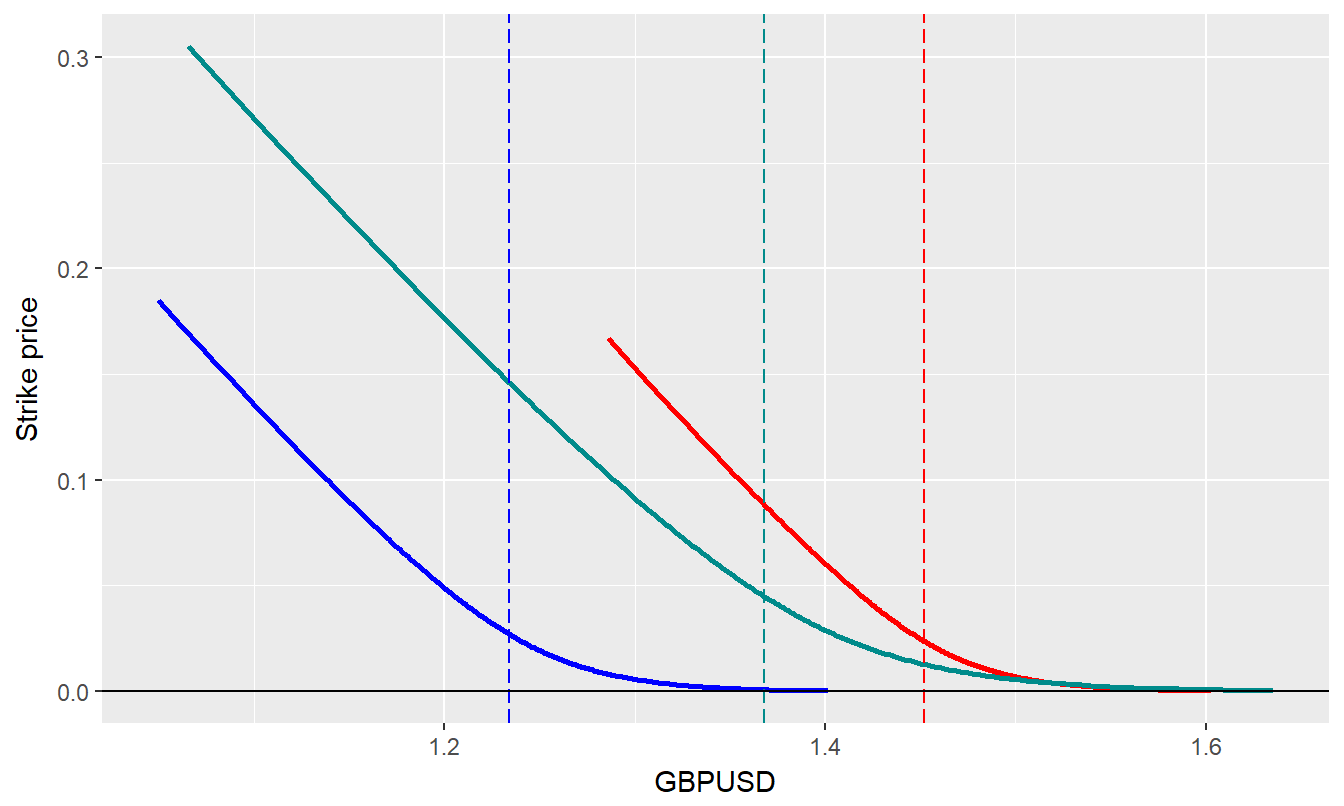
\includegraphics[width=1\linewidth]{images/unnamed-chunk-42-1} \caption{Call premium-strike functions}\label{fig:unnamed-chunk-42}
\end{figure}

Question: the call premium-strike functions are downward sloping,
i.e.~the call premium is higher for lower strike prices. Does this make
sense? Explain why.

\section{Generating put option
prices}\label{generating-put-option-prices}

Similarly, it is possible to obtain the put premium-strike function. The
corresponding commands to obtain the put premium are:

\begin{Shaded}
\begin{Highlighting}[]
\NormalTok{Put_preBrexit =}\StringTok{ }\KeywordTok{mapply}\NormalTok{(GKoption.premium, K_preBrexit, smile.df}\OperatorTok{$}\NormalTok{preBrexit,}
                        \DataTypeTok{S=}\NormalTok{spot[}\DecValTok{1}\NormalTok{],}\DataTypeTok{Tenor=}\NormalTok{Tenor,}\DataTypeTok{fwd=}\NormalTok{forward[}\DecValTok{1}\NormalTok{],}\DataTypeTok{rf=}\NormalTok{rf[}\DecValTok{1}\NormalTok{],}\DataTypeTok{option_type=}\StringTok{"p"}\NormalTok{)}

\NormalTok{Put_Brexit =}\StringTok{ }\KeywordTok{mapply}\NormalTok{(GKoption.premium, K_Brexit, smile.df}\OperatorTok{$}\NormalTok{Brexit,}
                        \DataTypeTok{S=}\NormalTok{spot[}\DecValTok{2}\NormalTok{],}\DataTypeTok{Tenor=}\NormalTok{Tenor,}\DataTypeTok{fwd=}\NormalTok{forward[}\DecValTok{2}\NormalTok{],}\DataTypeTok{rf=}\NormalTok{rf[}\DecValTok{2}\NormalTok{],}\DataTypeTok{option_type=}\StringTok{"p"}\NormalTok{)}

\NormalTok{Put_postBrexit =}\StringTok{ }\KeywordTok{mapply}\NormalTok{(GKoption.premium, K_postBrexit, smile.df}\OperatorTok{$}\NormalTok{postBrexit,}
                        \DataTypeTok{S=}\NormalTok{spot[}\DecValTok{3}\NormalTok{],}\DataTypeTok{Tenor=}\NormalTok{Tenor,}\DataTypeTok{fwd=}\NormalTok{forward[}\DecValTok{3}\NormalTok{],}\DataTypeTok{rf=}\NormalTok{rf[}\DecValTok{3}\NormalTok{],}\DataTypeTok{option_type=}\StringTok{"p"}\NormalTok{)}
\end{Highlighting}
\end{Shaded}

The needed data frame is:

\begin{Shaded}
\begin{Highlighting}[]
\NormalTok{putstrike.df =}\StringTok{ }\KeywordTok{data.frame}\NormalTok{(K_preBrexit, Put_preBrexit, K_Brexit, Put_Brexit, }
\NormalTok{                           K_postBrexit, Put_postBrexit)}
\end{Highlighting}
\end{Shaded}

and the plots are obtained with the following lines of code:

\begin{Shaded}
\begin{Highlighting}[]
\KeywordTok{ggplot}\NormalTok{(putstrike.df) }\OperatorTok{+}\StringTok{ }\KeywordTok{geom_line}\NormalTok{(}\KeywordTok{aes}\NormalTok{(}\DataTypeTok{x=}\NormalTok{K_preBrexit,}\DataTypeTok{y=}\NormalTok{Put_preBrexit), }\DataTypeTok{col=}\StringTok{"red"}\NormalTok{, }\DataTypeTok{size=}\DecValTok{1}\NormalTok{) }\OperatorTok{+}\StringTok{ }
\StringTok{  }\KeywordTok{geom_line}\NormalTok{(}\KeywordTok{aes}\NormalTok{(}\DataTypeTok{x=}\NormalTok{K_Brexit, }\DataTypeTok{y=}\NormalTok{Put_Brexit), }\DataTypeTok{col=}\StringTok{"darkcyan"}\NormalTok{, }\DataTypeTok{size=}\DecValTok{1}\NormalTok{) }\OperatorTok{+}
\StringTok{  }\KeywordTok{geom_line}\NormalTok{(}\KeywordTok{aes}\NormalTok{(}\DataTypeTok{x=}\NormalTok{K_postBrexit, }\DataTypeTok{y=}\NormalTok{Put_postBrexit), }\DataTypeTok{col=}\StringTok{"blue"}\NormalTok{, }\DataTypeTok{size=}\DecValTok{1}\NormalTok{) }\OperatorTok{+}
\StringTok{  }\KeywordTok{labs}\NormalTok{(}\DataTypeTok{x=}\StringTok{"Strike price"}\NormalTok{, }\DataTypeTok{y=}\StringTok{"Put premium"}\NormalTok{) }\OperatorTok{+}\StringTok{ }
\StringTok{  }\KeywordTok{geom_vline}\NormalTok{(}\DataTypeTok{xintercept =}\NormalTok{ spot[}\DecValTok{1}\NormalTok{], }\DataTypeTok{col=}\StringTok{"red"}\NormalTok{, }\DataTypeTok{linetype=}\StringTok{"longdash"}\NormalTok{) }\OperatorTok{+}\StringTok{ }
\StringTok{  }\KeywordTok{geom_vline}\NormalTok{(}\DataTypeTok{xintercept =}\NormalTok{ spot[}\DecValTok{2}\NormalTok{], }\DataTypeTok{col=}\StringTok{"darkcyan"}\NormalTok{, }\DataTypeTok{linetype=}\StringTok{"longdash"}\NormalTok{) }\OperatorTok{+}
\StringTok{  }\KeywordTok{geom_vline}\NormalTok{(}\DataTypeTok{xintercept =}\NormalTok{ spot[}\DecValTok{3}\NormalTok{], }\DataTypeTok{col=}\StringTok{"blue"}\NormalTok{, }\DataTypeTok{linetype=}\StringTok{"longdash"}\NormalTok{) }\OperatorTok{+}
\StringTok{  }\KeywordTok{geom_hline}\NormalTok{(}\DataTypeTok{yintercept =} \DecValTok{0}\NormalTok{, }\DataTypeTok{col=}\StringTok{"black"}\NormalTok{)}
\end{Highlighting}
\end{Shaded}

\begin{figure}
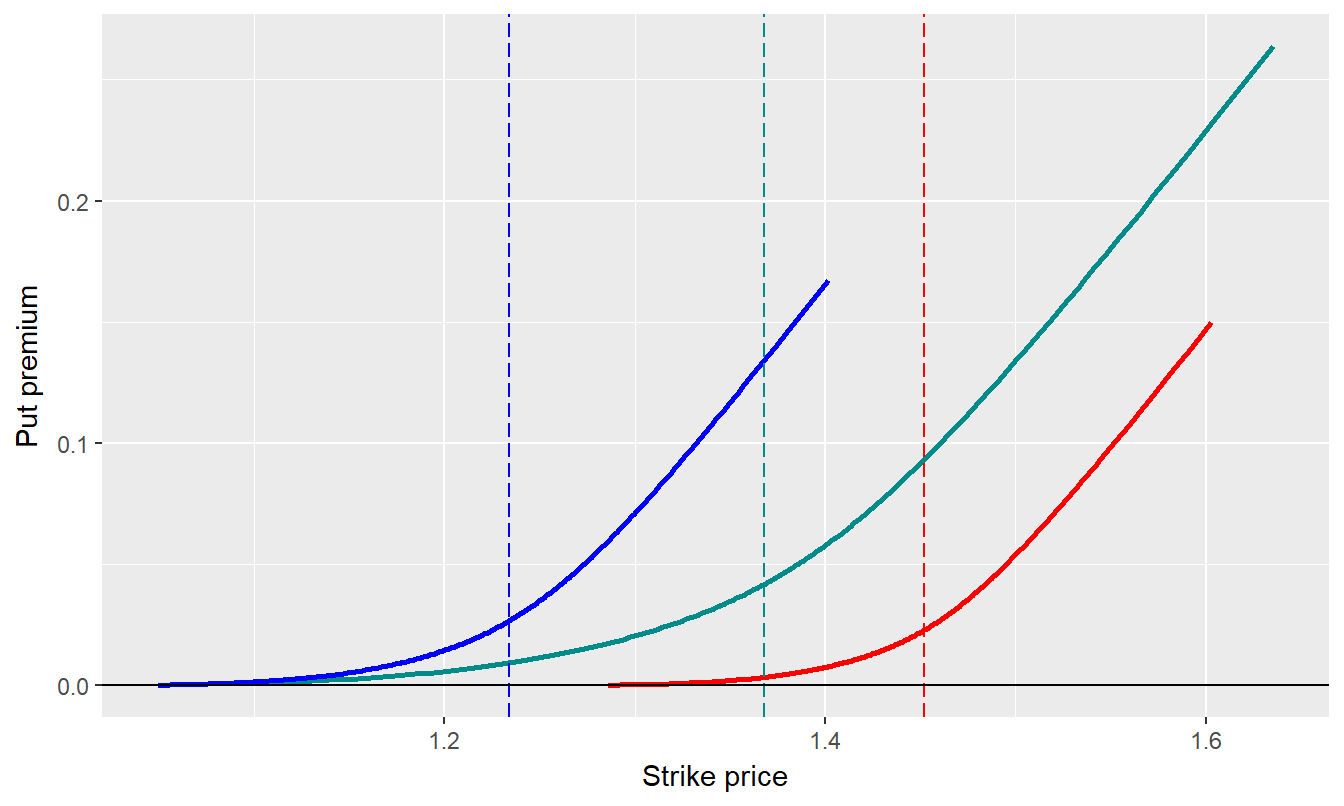
\includegraphics[width=1\linewidth]{images/unnamed-chunk-45-1} \caption{Put premium-strike functions}\label{fig:unnamed-chunk-45}
\end{figure}

\section{Practical Implementation}\label{practical-implementation}

Once the premium-strike functions are calculated, Hamidieh's
\textbf{\texttt{RND}} package serves to estimate the risk-neutral
densities \citep{R-RND}. The package implements a number of
non-structural estimation methods. Payne estimated the risk-neutral
density using the following methods:

\begin{itemize}
\tightlist
\item
  Generalized beta density (parametric).
\item
  Edgeworth expansion (semi-parametric).
\item
  the Shimko method (non-parametric).
\end{itemize}

Parametric methods based on fitting a probability distribution to the
data generate smooth distributions, especially compared to
non-parametric methods based on the numerical computation of the second
derivative of the premium-strike function. To examine this claim, we
will replicate Payne's calculations. Start by loading the package
\textbf{\texttt{RND}} into memory:

\begin{Shaded}
\begin{Highlighting}[]
\KeywordTok{library}\NormalTok{(RND)}
\end{Highlighting}
\end{Shaded}

\section{Generalized beta
distribution}\label{generalized-beta-distribution}

The generalized beta distribution, introduced in option pricing by
\citet{Bookstaber-McDonald1987}, is very flexible, and can accommodate
asymmetries and a wide variety of fat tails. The \texttt{RND}
implementation of the generalized beta distribution requires a number of
inputs. To illustrate it, we start by extracting the distribution for
the pre-Brexit date:

\begin{Shaded}
\begin{Highlighting}[]
\CommentTok{# Input for inferring the generalized beta distribution in the pre-Brexit period}

\NormalTok{r =}\StringTok{ }\NormalTok{imp_rd[}\DecValTok{1}\NormalTok{]                      }\CommentTok{# domestic interest rate}
\NormalTok{te=}\StringTok{ }\NormalTok{Tenor                          }\CommentTok{# tenor of the option}
\NormalTok{y =}\StringTok{ }\NormalTok{rf[}\DecValTok{1}\NormalTok{]                          }\CommentTok{# foreign interest rate}
\NormalTok{s0=}\StringTok{ }\NormalTok{spot[}\DecValTok{1}\NormalTok{]                        }\CommentTok{# spot exchange rate}
\NormalTok{call.premium =}\StringTok{ }\NormalTok{Call_preBrexit      }\CommentTok{# vector of call premium values}
\NormalTok{call.strikes =}\StringTok{ }\NormalTok{K_preBrexit         }\CommentTok{# vector of corresponding call strikes}
\NormalTok{put.premium =}\StringTok{ }\NormalTok{Put_preBrexit        }\CommentTok{# vector of put premium values}
\NormalTok{put.strikes =}\StringTok{ }\NormalTok{K_preBrexit          }\CommentTok{# vector of corresponding put strikes}
\end{Highlighting}
\end{Shaded}

Note that we do not use the observed domestic interest rate but rather
the implied rate from the forward exchange rate. This choice is
consistent with the pricing formulas used to infer the strike and
premium, both of which were based in the forward rate.

To extract the distribution, we use the function
\texttt{extract.gb.density()}:

\begin{Shaded}
\begin{Highlighting}[]
\NormalTok{gb.preBrexit =}\StringTok{ }\KeywordTok{extract.gb.density}\NormalTok{(}\DataTypeTok{initial.values=}\KeywordTok{c}\NormalTok{(}\OtherTok{NA}\NormalTok{,}\OtherTok{NA}\NormalTok{,}\OtherTok{NA}\NormalTok{,}\OtherTok{NA}\NormalTok{), }\DataTypeTok{r=}\NormalTok{r, }\DataTypeTok{te=}\NormalTok{te, }\DataTypeTok{y=}\NormalTok{y, }\DataTypeTok{s0=}\NormalTok{s0, }
                       \DataTypeTok{market.calls=}\NormalTok{call.premium, }\DataTypeTok{call.strikes =}\NormalTok{ call.strikes, }\DataTypeTok{call.weights =}\DecValTok{1}\NormalTok{,}
                       \DataTypeTok{market.puts =}\NormalTok{ put.premium, }\DataTypeTok{put.strikes =}\NormalTok{ put.strikes, }\DataTypeTok{put.weights =} \DecValTok{1}\NormalTok{,  }
                       \DataTypeTok{lambda=}\DecValTok{1}\NormalTok{, }\DataTypeTok{hessian.flag=}\NormalTok{F)}
\end{Highlighting}
\end{Shaded}

The parameters \texttt{call.weights} and \texttt{put.weights} are set
equal to 1, as there is no evidence that either type of options should
weight more heavily when inferring the distribution. The penalty
parameter \texttt{lambda} should be set equal to 1 always.

The object \texttt{gb.preBrexit} contains the parameters of the
generalized beta distribution, \texttt{a}, \texttt{b}, \texttt{v}, and
\texttt{w}. To obtain the risk neutral density, we first set a range of
strike prices, \texttt{Krange}:

\begin{Shaded}
\begin{Highlighting}[]
\NormalTok{Krange =}\StringTok{ }\KeywordTok{seq}\NormalTok{(}\FloatTok{0.9}\OperatorTok{*}\KeywordTok{min}\NormalTok{(K_preBrexit, K_Brexit, K_postBrexit), }\FloatTok{1.1}\OperatorTok{*}\KeywordTok{max}\NormalTok{(K_preBrexit, K_Brexit, K_postBrexit), }\FloatTok{0.01}\NormalTok{)}
\end{Highlighting}
\end{Shaded}

and then use the function \texttt{dgb()} to obtain the risk neutral
distribution using as inputs the estimated distribution parameters:

\begin{Shaded}
\begin{Highlighting}[]
\NormalTok{gb =}\StringTok{ }\NormalTok{gb.preBrexit}
\NormalTok{gb.rnd.preBrexit =}\StringTok{ }\KeywordTok{dgb}\NormalTok{(Krange,gb}\OperatorTok{$}\NormalTok{a, gb}\OperatorTok{$}\NormalTok{b, gb}\OperatorTok{$}\NormalTok{v, gb}\OperatorTok{$}\NormalTok{w)}
\end{Highlighting}
\end{Shaded}

We repeat the calculations for the Brexit date:

\begin{Shaded}
\begin{Highlighting}[]
\NormalTok{r =}\StringTok{ }\NormalTok{imp_rd[}\DecValTok{2}\NormalTok{]}
\NormalTok{y =}\StringTok{ }\NormalTok{rf[}\DecValTok{2}\NormalTok{]}
\NormalTok{s0=}\StringTok{ }\NormalTok{spot[}\DecValTok{2}\NormalTok{]}
\NormalTok{call.premium =}\StringTok{ }\NormalTok{Call_Brexit}
\NormalTok{call.strikes =}\StringTok{ }\NormalTok{K_Brexit}
\NormalTok{put.premium =}\StringTok{ }\NormalTok{Put_Brexit}
\NormalTok{put.strikes =}\StringTok{ }\NormalTok{K_Brexit}

\NormalTok{gb.Brexit =}\StringTok{ }\KeywordTok{extract.gb.density}\NormalTok{(}\DataTypeTok{initial.values=}\KeywordTok{c}\NormalTok{(}\OtherTok{NA}\NormalTok{,}\OtherTok{NA}\NormalTok{,}\OtherTok{NA}\NormalTok{,}\OtherTok{NA}\NormalTok{), }\DataTypeTok{r=}\NormalTok{r, }\DataTypeTok{te=}\NormalTok{te, }\DataTypeTok{y=}\NormalTok{y, }\DataTypeTok{s0=}\NormalTok{s0, }
                       \DataTypeTok{market.calls=}\NormalTok{call.premium, }\DataTypeTok{call.strikes =}\NormalTok{ call.strikes, }\DataTypeTok{call.weights =}\DecValTok{1}\NormalTok{,}
                       \DataTypeTok{market.puts =}\NormalTok{ put.premium, }\DataTypeTok{put.strikes =}\NormalTok{ put.strikes, }\DataTypeTok{put.weights =} \DecValTok{1}\NormalTok{,  }
                       \DataTypeTok{lambda=}\DecValTok{1}\NormalTok{, }\DataTypeTok{hessian.flag=}\NormalTok{F)}

\NormalTok{gb =}\StringTok{ }\NormalTok{gb.Brexit}
\NormalTok{gb.rnd.Brexit =}\StringTok{ }\KeywordTok{dgb}\NormalTok{(Krange,gb}\OperatorTok{$}\NormalTok{a, gb}\OperatorTok{$}\NormalTok{b, gb}\OperatorTok{$}\NormalTok{v, gb}\OperatorTok{$}\NormalTok{w)}
\end{Highlighting}
\end{Shaded}

and post-Brexit dates:

\begin{Shaded}
\begin{Highlighting}[]
\NormalTok{r =}\StringTok{ }\NormalTok{imp_rd[}\DecValTok{3}\NormalTok{]}
\NormalTok{y =}\StringTok{ }\NormalTok{rf[}\DecValTok{3}\NormalTok{]}
\NormalTok{s0=}\StringTok{ }\NormalTok{spot[}\DecValTok{3}\NormalTok{]}
\NormalTok{call.premium =}\StringTok{ }\NormalTok{Call_postBrexit}
\NormalTok{call.strikes =}\StringTok{ }\NormalTok{K_postBrexit}
\NormalTok{put.premium =}\StringTok{ }\NormalTok{Put_postBrexit}
\NormalTok{put.strikes =}\StringTok{ }\NormalTok{K_postBrexit}

\NormalTok{gb.postBrexit =}\StringTok{ }\KeywordTok{extract.gb.density}\NormalTok{(}\DataTypeTok{initial.values=}\KeywordTok{c}\NormalTok{(}\OtherTok{NA}\NormalTok{,}\OtherTok{NA}\NormalTok{,}\OtherTok{NA}\NormalTok{,}\OtherTok{NA}\NormalTok{), }\DataTypeTok{r=}\NormalTok{r, }\DataTypeTok{te=}\NormalTok{te, }\DataTypeTok{y=}\NormalTok{y, }\DataTypeTok{s0=}\NormalTok{s0, }
                        \DataTypeTok{market.calls=}\NormalTok{call.premium, }\DataTypeTok{call.strikes =}\NormalTok{ call.strikes, }\DataTypeTok{call.weights =}\DecValTok{1}\NormalTok{,}
                        \DataTypeTok{market.puts =}\NormalTok{ put.premium, }\DataTypeTok{put.strikes =}\NormalTok{ put.strikes, }\DataTypeTok{put.weights =} \DecValTok{1}\NormalTok{,  }
                        \DataTypeTok{lambda=}\DecValTok{1}\NormalTok{, }\DataTypeTok{hessian.flag=}\NormalTok{F)}

\NormalTok{gb =}\StringTok{ }\NormalTok{gb.postBrexit}
\NormalTok{gb.rnd.postBrexit =}\StringTok{ }\KeywordTok{dgb}\NormalTok{(Krange,gb}\OperatorTok{$}\NormalTok{a, gb}\OperatorTok{$}\NormalTok{b, gb}\OperatorTok{$}\NormalTok{v, gb}\OperatorTok{$}\NormalTok{w)}
\end{Highlighting}
\end{Shaded}

To compare the risk-neutral distributions, we create the data frame
\texttt{gb.rnd.df}, and proceed to plot them using \texttt{ggplot}:

\begin{Shaded}
\begin{Highlighting}[]
\NormalTok{gb.rnd.df =}\StringTok{ }\KeywordTok{data.frame}\NormalTok{(Krange,gb.rnd.preBrexit, gb.rnd.Brexit, gb.rnd.postBrexit)}

\KeywordTok{ggplot}\NormalTok{(}\DataTypeTok{data=}\NormalTok{gb.rnd.df, }\KeywordTok{aes}\NormalTok{(}\DataTypeTok{x=}\NormalTok{Krange)) }\OperatorTok{+}\StringTok{ }\KeywordTok{geom_line}\NormalTok{(}\KeywordTok{aes}\NormalTok{(}\DataTypeTok{y=}\NormalTok{gb.rnd.preBrexit), }\DataTypeTok{col=}\StringTok{"red"}\NormalTok{, }\DataTypeTok{size=}\FloatTok{1.25}\NormalTok{) }\OperatorTok{+}
\StringTok{  }\KeywordTok{geom_line}\NormalTok{(}\KeywordTok{aes}\NormalTok{(}\DataTypeTok{y=}\NormalTok{gb.rnd.Brexit), }\DataTypeTok{col=}\StringTok{"darkcyan"}\NormalTok{, }\DataTypeTok{size=}\FloatTok{1.25}\NormalTok{) }\OperatorTok{+}
\StringTok{  }\KeywordTok{geom_line}\NormalTok{(}\KeywordTok{aes}\NormalTok{(}\DataTypeTok{y=}\NormalTok{gb.rnd.postBrexit), }\DataTypeTok{col=}\StringTok{"blue"}\NormalTok{, }\DataTypeTok{size=}\FloatTok{1.25}\NormalTok{) }\OperatorTok{+}
\StringTok{  }\KeywordTok{geom_vline}\NormalTok{(}\DataTypeTok{xintercept =}\NormalTok{ spot[}\DecValTok{1}\NormalTok{], }\DataTypeTok{col=}\StringTok{"red"}\NormalTok{, }\DataTypeTok{linetype=}\StringTok{"longdash"}\NormalTok{) }\OperatorTok{+}\StringTok{ }
\StringTok{  }\KeywordTok{geom_vline}\NormalTok{(}\DataTypeTok{xintercept =}\NormalTok{ spot[}\DecValTok{2}\NormalTok{], }\DataTypeTok{col=}\StringTok{"darkcyan"}\NormalTok{, }\DataTypeTok{linetype=}\StringTok{"longdash"}\NormalTok{) }\OperatorTok{+}
\StringTok{  }\KeywordTok{geom_vline}\NormalTok{(}\DataTypeTok{xintercept =}\NormalTok{ spot[}\DecValTok{3}\NormalTok{], }\DataTypeTok{col=}\StringTok{"blue"}\NormalTok{, }\DataTypeTok{linetype=}\StringTok{"longdash"}\NormalTok{) }\OperatorTok{+}
\StringTok{  }\KeywordTok{geom_hline}\NormalTok{(}\DataTypeTok{yintercept=}\DecValTok{0}\NormalTok{, }\DataTypeTok{col=}\StringTok{"black"}\NormalTok{, }\DataTypeTok{size=}\FloatTok{0.5}\NormalTok{) }\OperatorTok{+}
\StringTok{  }\KeywordTok{labs}\NormalTok{(}\DataTypeTok{x=}\StringTok{"GBPUSD"}\NormalTok{, }\DataTypeTok{y=}\StringTok{"3-month risk-neutral density"}\NormalTok{)   }
\end{Highlighting}
\end{Shaded}

\begin{figure}
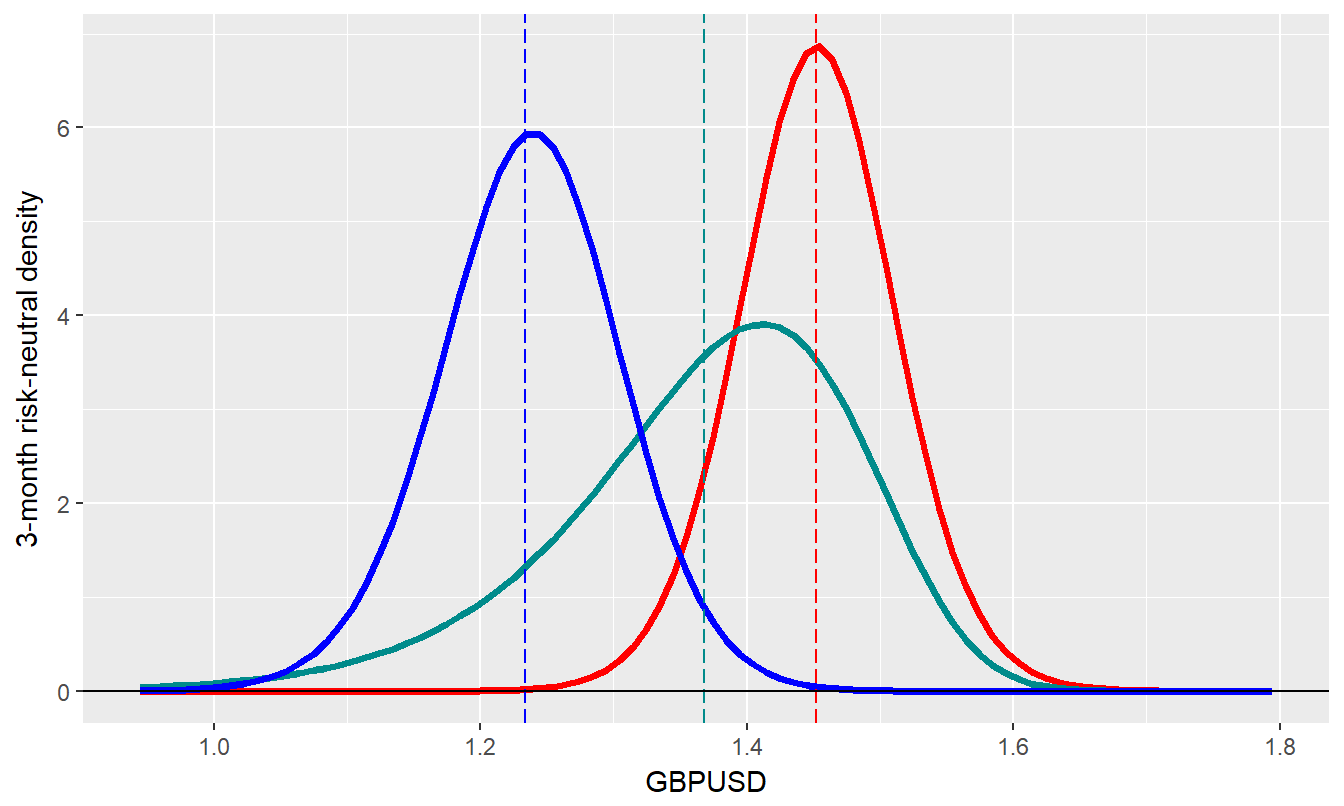
\includegraphics[width=1\linewidth]{images/unnamed-chunk-53-1} \caption{Generalized beta risk neutral distributions.</br>Pre-Brexit: red; Brexit: cyan; post-Brexit: blue}\label{fig:unnamed-chunk-53}
\end{figure}

\section{Edgeworth expansion}\label{edgeworth-expansion}

\citet{Jarrow-Rudd1982} model the risk-neutral distribution by modifying
the log-normal distribution using an Edgeworth expansion. Payne knew
about a good reference on the latter topic, \citet{Hall1992}, but
decided to put off reading it. She was fully aware that her next salary
increase and promotion was at most weakly correlated with her technical
knowledge. Rather the correlation was way stronger with the number of
policy notes she could put together.

So Payne put her best efforts to get the figures for her policy note.
She started by calculating the risk neutral distributions for the
pre-Brexit period. To replicate her work, we first collect the required
input:

\begin{Shaded}
\begin{Highlighting}[]
\NormalTok{r =}\StringTok{ }\NormalTok{imp_rd[}\DecValTok{1}\NormalTok{]                      }\CommentTok{# domestic interest rate}
\NormalTok{te=}\StringTok{ }\NormalTok{Tenor                          }\CommentTok{# tenor of the option}
\NormalTok{y =}\StringTok{ }\NormalTok{rf[}\DecValTok{1}\NormalTok{]                          }\CommentTok{# foreign interest rate}
\NormalTok{s0=}\StringTok{ }\NormalTok{spot[}\DecValTok{1}\NormalTok{]                        }\CommentTok{# spot exchange rate}
\NormalTok{call.premium =}\StringTok{ }\NormalTok{Call_preBrexit      }\CommentTok{# vector of call premium values}
\NormalTok{call.strikes =}\StringTok{ }\NormalTok{K_preBrexit         }\CommentTok{# vector of corresponding call strikes}
\end{Highlighting}
\end{Shaded}

The function \texttt{extract.ew.density()} calculates the parameters of
the Edgeworth expansion:

\begin{Shaded}
\begin{Highlighting}[]
\NormalTok{ew.preBrexit =}\StringTok{ }\KeywordTok{extract.ew.density}\NormalTok{(}\DataTypeTok{initial.values =} \KeywordTok{rep}\NormalTok{(}\OtherTok{NA}\NormalTok{,}\DecValTok{2}\NormalTok{), }\DataTypeTok{r=}\NormalTok{r, }\DataTypeTok{y=}\NormalTok{y, }\DataTypeTok{te=}\NormalTok{te, }\DataTypeTok{s0=}\NormalTok{s0, }
                       \DataTypeTok{market.calls=}\NormalTok{call.premium, }\DataTypeTok{call.strikes =}\NormalTok{ call.strikes, }
                       \DataTypeTok{call.weights =}\DecValTok{1}\NormalTok{, }\DataTypeTok{lambda=}\DecValTok{1}\NormalTok{, }\DataTypeTok{hessian.flag=}\NormalTok{F, }\DataTypeTok{cl =} \KeywordTok{list}\NormalTok{(}\DataTypeTok{maxit=}\DecValTok{10000}\NormalTok{))}
\end{Highlighting}
\end{Shaded}

which we then input into the function \texttt{dew()} to obtain the
distribution.

\begin{Shaded}
\begin{Highlighting}[]
\NormalTok{ew =}\StringTok{ }\NormalTok{ew.preBrexit}
\NormalTok{ew.rnd.preBrexit  =}\StringTok{ }\KeywordTok{dew}\NormalTok{(Krange,r,y,te,s0,ew}\OperatorTok{$}\NormalTok{sigma, ew}\OperatorTok{$}\NormalTok{skew, ew}\OperatorTok{$}\NormalTok{kurt)}
\end{Highlighting}
\end{Shaded}

Let's do this for the two other periods, Brexit:

\begin{Shaded}
\begin{Highlighting}[]
\NormalTok{r =}\StringTok{ }\NormalTok{imp_rd[}\DecValTok{2}\NormalTok{]                      }\CommentTok{# domestic interest rate}
\NormalTok{te=}\StringTok{ }\NormalTok{Tenor                          }\CommentTok{# tenor of the option}
\NormalTok{y =}\StringTok{ }\NormalTok{rf[}\DecValTok{2}\NormalTok{]                          }\CommentTok{# foreign interest rate}
\NormalTok{s0=}\StringTok{ }\NormalTok{spot[}\DecValTok{2}\NormalTok{]                        }\CommentTok{# spot exchange rate}
\NormalTok{call.premium =}\StringTok{ }\NormalTok{Call_Brexit         }\CommentTok{# vector of call premium values}
\NormalTok{call.strikes =}\StringTok{ }\NormalTok{K_Brexit            }\CommentTok{# vector of corresponding call strikes}

\NormalTok{ew.Brexit =}\StringTok{ }\KeywordTok{extract.ew.density}\NormalTok{(}\DataTypeTok{initial.values =} \KeywordTok{rep}\NormalTok{(}\OtherTok{NA}\NormalTok{,}\DecValTok{2}\NormalTok{), }\DataTypeTok{r=}\NormalTok{r, }\DataTypeTok{y=}\NormalTok{y, }\DataTypeTok{te=}\NormalTok{te, }\DataTypeTok{s0=}\NormalTok{s0, }
                    \DataTypeTok{market.calls=}\NormalTok{call.premium, }\DataTypeTok{call.strikes =}\NormalTok{ call.strikes, }
                    \DataTypeTok{call.weights =}\DecValTok{1}\NormalTok{, }\DataTypeTok{lambda=}\DecValTok{1}\NormalTok{, }\DataTypeTok{hessian.flag=}\NormalTok{F,   }\DataTypeTok{cl =} \KeywordTok{list}\NormalTok{(}\DataTypeTok{maxit=}\DecValTok{10000}\NormalTok{))}
\NormalTok{ew =}\StringTok{ }\NormalTok{ew.Brexit}
\NormalTok{ew.rnd.Brexit  =}\StringTok{ }\KeywordTok{dew}\NormalTok{(Krange,r,y,te,s0,ew}\OperatorTok{$}\NormalTok{sigma, ew}\OperatorTok{$}\NormalTok{skew, ew}\OperatorTok{$}\NormalTok{kurt)}
\end{Highlighting}
\end{Shaded}

and post-Brexit:

\begin{Shaded}
\begin{Highlighting}[]
\NormalTok{r =}\StringTok{ }\NormalTok{imp_rd[}\DecValTok{3}\NormalTok{]                      }\CommentTok{# domestic interest rate}
\NormalTok{te=}\StringTok{ }\NormalTok{Tenor                          }\CommentTok{# tenor of the option}
\NormalTok{y =}\StringTok{ }\NormalTok{rf[}\DecValTok{3}\NormalTok{]                          }\CommentTok{# foreign interest rate}
\NormalTok{s0=}\StringTok{ }\NormalTok{spot[}\DecValTok{3}\NormalTok{]                        }\CommentTok{# spot exchange rate}
\NormalTok{call.premium =}\StringTok{ }\NormalTok{Call_postBrexit     }\CommentTok{# vector of call premium values}
\NormalTok{call.strikes =}\StringTok{ }\NormalTok{K_postBrexit        }\CommentTok{# vector of corresponding call strikes}

\NormalTok{ew.postBrexit =}\StringTok{ }\KeywordTok{extract.ew.density}\NormalTok{(}\DataTypeTok{initial.values =} \KeywordTok{rep}\NormalTok{(}\OtherTok{NA}\NormalTok{,}\DecValTok{2}\NormalTok{), }\DataTypeTok{r=}\NormalTok{r, }\DataTypeTok{y=}\NormalTok{y, }\DataTypeTok{te=}\NormalTok{te, }\DataTypeTok{s0=}\NormalTok{s0, }
                        \DataTypeTok{market.calls=}\NormalTok{call.premium, }\DataTypeTok{call.strikes =}\NormalTok{ call.strikes, }
                        \DataTypeTok{call.weights =}\DecValTok{1}\NormalTok{, }\DataTypeTok{lambda=}\DecValTok{1}\NormalTok{, }\DataTypeTok{hessian.flag=}\NormalTok{F, }\DataTypeTok{cl =} \KeywordTok{list}\NormalTok{(}\DataTypeTok{maxit=}\DecValTok{10000}\NormalTok{))}
\NormalTok{ew =}\StringTok{ }\NormalTok{ew.postBrexit}
\NormalTok{ew.rnd.postBrexit  =}\StringTok{ }\KeywordTok{dew}\NormalTok{(Krange,r,y,te,s0,ew}\OperatorTok{$}\NormalTok{sigma, ew}\OperatorTok{$}\NormalTok{skew, ew}\OperatorTok{$}\NormalTok{kurt)}
\end{Highlighting}
\end{Shaded}

To generate the plot, issue these commands:

\begin{Shaded}
\begin{Highlighting}[]
\NormalTok{ew.rnd.df =}\StringTok{ }\KeywordTok{data.frame}\NormalTok{(Krange, ew.rnd.preBrexit, ew.rnd.Brexit, ew.rnd.postBrexit)}

\KeywordTok{ggplot}\NormalTok{(}\DataTypeTok{data=}\NormalTok{ew.rnd.df, }\KeywordTok{aes}\NormalTok{(}\DataTypeTok{x=}\NormalTok{Krange)) }\OperatorTok{+}\StringTok{ }\KeywordTok{geom_line}\NormalTok{(}\KeywordTok{aes}\NormalTok{(}\DataTypeTok{y=}\NormalTok{ew.rnd.preBrexit), }\DataTypeTok{col=}\StringTok{"red"}\NormalTok{, }\DataTypeTok{size=}\FloatTok{1.25}\NormalTok{) }\OperatorTok{+}
\StringTok{  }\KeywordTok{geom_line}\NormalTok{(}\KeywordTok{aes}\NormalTok{(}\DataTypeTok{y=}\NormalTok{ew.rnd.Brexit), }\DataTypeTok{col=}\StringTok{"darkcyan"}\NormalTok{, }\DataTypeTok{size=}\FloatTok{1.25}\NormalTok{) }\OperatorTok{+}
\StringTok{  }\KeywordTok{geom_line}\NormalTok{(}\KeywordTok{aes}\NormalTok{(}\DataTypeTok{y=}\NormalTok{ew.rnd.postBrexit), }\DataTypeTok{col=}\StringTok{"blue"}\NormalTok{, }\DataTypeTok{size=}\FloatTok{1.25}\NormalTok{) }\OperatorTok{+}
\StringTok{  }\KeywordTok{geom_vline}\NormalTok{(}\DataTypeTok{xintercept =}\NormalTok{ spot[}\DecValTok{1}\NormalTok{], }\DataTypeTok{col=}\StringTok{"red"}\NormalTok{, }\DataTypeTok{linetype=}\StringTok{"longdash"}\NormalTok{) }\OperatorTok{+}\StringTok{ }
\StringTok{  }\KeywordTok{geom_vline}\NormalTok{(}\DataTypeTok{xintercept =}\NormalTok{ spot[}\DecValTok{2}\NormalTok{], }\DataTypeTok{col=}\StringTok{"darkcyan"}\NormalTok{, }\DataTypeTok{linetype=}\StringTok{"longdash"}\NormalTok{) }\OperatorTok{+}
\StringTok{  }\KeywordTok{geom_vline}\NormalTok{(}\DataTypeTok{xintercept =}\NormalTok{ spot[}\DecValTok{3}\NormalTok{], }\DataTypeTok{col=}\StringTok{"blue"}\NormalTok{, }\DataTypeTok{linetype=}\StringTok{"longdash"}\NormalTok{) }\OperatorTok{+}
\StringTok{  }\KeywordTok{geom_hline}\NormalTok{(}\DataTypeTok{yintercept=}\DecValTok{0}\NormalTok{, }\DataTypeTok{col=}\StringTok{"black"}\NormalTok{, }\DataTypeTok{size=}\FloatTok{0.5}\NormalTok{) }\OperatorTok{+}
\StringTok{  }\KeywordTok{labs}\NormalTok{(}\DataTypeTok{x=}\StringTok{"GBPUSD"}\NormalTok{, }\DataTypeTok{y=}\StringTok{"3-month risk-neutral density"}\NormalTok{)   }
\end{Highlighting}
\end{Shaded}

\begin{figure}
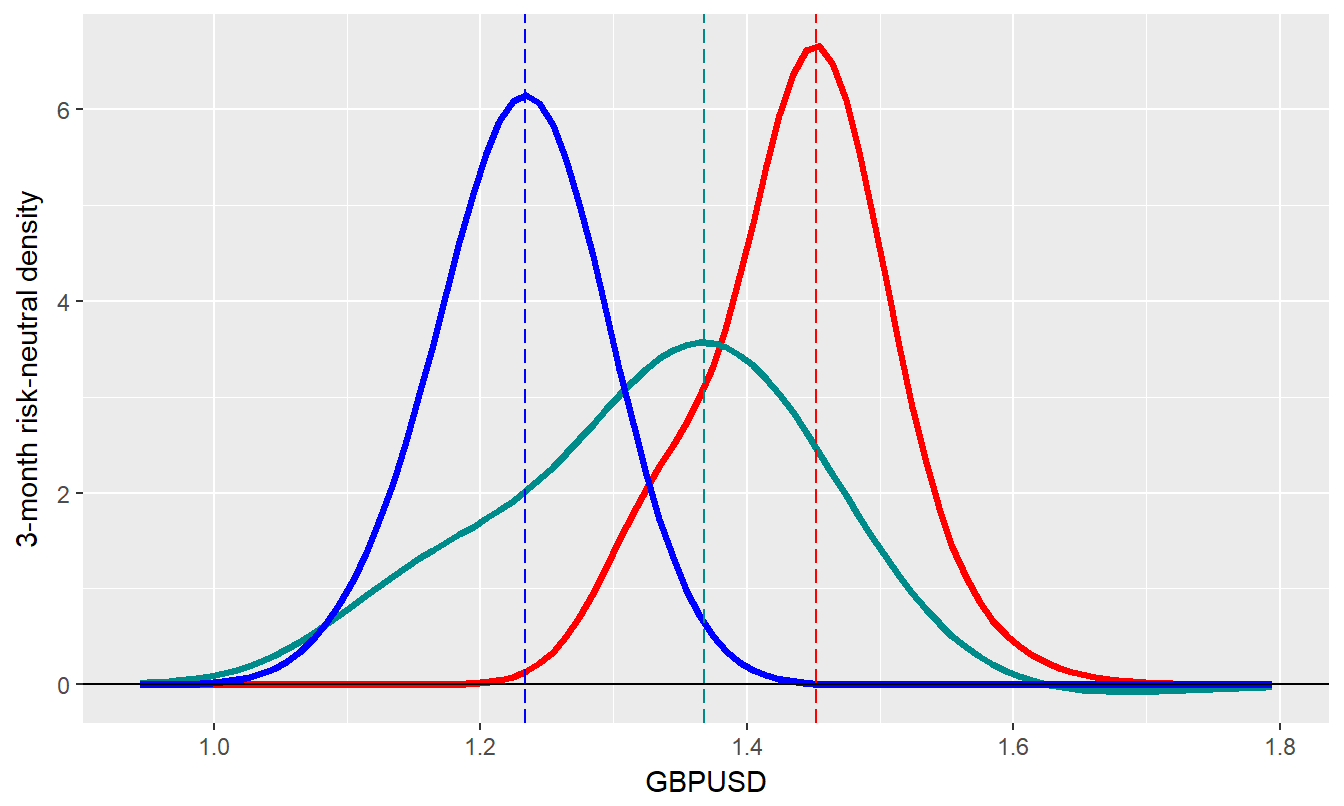
\includegraphics[width=1\linewidth]{images/unnamed-chunk-59-1} \caption{Edgeworth expansion risk neutral distributions.</br>Pre-Brexit: red; Brexit: cyan; post-Brexit: blue}\label{fig:unnamed-chunk-59}
\end{figure}

\section{Shimko method}\label{shimko-method}

The method first calculates an implied probability function linking
implied volatilities to strike prices \citep{Shimko1993}. The function
is then used to obtain the call premium-strike price function. Following
Breeden and Litzenberger, the risk neutral density is obtained obtaining
the second derivative of the call premium-strike price function
numerically.

To calculate the Shimko density in the pre-Brexit date, we first need to
find the strike prices, in terms of exchange rate values, for the
10\(\Delta\), 25\(\Delta\), 50\(\Delta\), 75\(\Delta\) and 90\(\Delta\)
strikes, and match them with the corresponding call premia:

\begin{Shaded}
\begin{Highlighting}[]
\NormalTok{vol.preBrexit =}\StringTok{ }\NormalTok{vol.data[}\DecValTok{1}\OperatorTok{:}\DecValTok{5}\NormalTok{,}\DecValTok{3}\NormalTok{]         }\CommentTok{# obtain implied volatility}
\NormalTok{delta.shimko =}\StringTok{ }\NormalTok{vol.data[}\DecValTok{1}\OperatorTok{:}\DecValTok{5}\NormalTok{,}\DecValTok{1}\NormalTok{]          }\CommentTok{# obtain the deltas}

\CommentTok{# Calculate the strike prices corresponding to the observed deltas}

\NormalTok{Kshimko_preBrexit =}\StringTok{ }\KeywordTok{mapply}\NormalTok{(get.strike,vol.preBrexit, delta.shimko,}
                     \DataTypeTok{S0=}\NormalTok{spot[}\DecValTok{1}\NormalTok{], }\DataTypeTok{fwd=}\NormalTok{forward[}\DecValTok{1}\NormalTok{], }\DataTypeTok{rf=}\NormalTok{rf[}\DecValTok{1}\NormalTok{], }\DataTypeTok{Tenor=}\FloatTok{0.25}\NormalTok{)}

\CommentTok{# Calculate the call premium for the observed deltas and corresponding strikes}

\NormalTok{shimko_preBrexit =}\StringTok{ }\KeywordTok{mapply}\NormalTok{(GKoption.premium, Kshimko_preBrexit, vol.preBrexit,}
                        \DataTypeTok{S=}\NormalTok{spot[}\DecValTok{1}\NormalTok{],}\DataTypeTok{Tenor=}\NormalTok{Tenor,}\DataTypeTok{fwd=}\NormalTok{forward[}\DecValTok{1}\NormalTok{],}\DataTypeTok{rf=}\NormalTok{rf[}\DecValTok{1}\NormalTok{],}\DataTypeTok{option_type=}\StringTok{"c"}\NormalTok{)}
\end{Highlighting}
\end{Shaded}

The function in the \texttt{RND} package that calculates the parameters
of the Shimko's quadratic approximation to the volatility smile is
\texttt{extract.shimko.density()}:

\begin{Shaded}
\begin{Highlighting}[]
\CommentTok{# Inputs for extract.shimko.density()}

\NormalTok{r =}\StringTok{ }\NormalTok{imp_rd[}\DecValTok{1}\NormalTok{]                      }\CommentTok{# implied doomestic rate}
\NormalTok{te=}\StringTok{ }\NormalTok{Tenor                          }\CommentTok{# time to  maturity}
\NormalTok{y =}\StringTok{ }\NormalTok{rf[}\DecValTok{1}\NormalTok{]                          }\CommentTok{# foreign interest rate}
\NormalTok{s0=}\StringTok{ }\NormalTok{spot[}\DecValTok{1}\NormalTok{]                        }\CommentTok{# spot exchange rate}
\NormalTok{call.premium =}\StringTok{ }\NormalTok{shimko_preBrexit    }\CommentTok{# call premia values}
\NormalTok{call.strikes =}\StringTok{ }\NormalTok{Kshimko_preBrexit   }\CommentTok{# option strikes}
\NormalTok{b=r}\OperatorTok{-}\NormalTok{y}

\NormalTok{shimko.preBrexit =}\StringTok{ }\KeywordTok{extract.shimko.density}\NormalTok{(}\DataTypeTok{market.calls=}\NormalTok{call.premium, }\DataTypeTok{call.strikes =}\NormalTok{ call.strikes, }
                                   \DataTypeTok{r=}\NormalTok{r, }\DataTypeTok{y=}\NormalTok{b, }\DataTypeTok{t=}\NormalTok{te, }\DataTypeTok{s0=}\NormalTok{s0, }\DataTypeTok{lower=}\DecValTok{0}\NormalTok{, }\DataTypeTok{upper=} \DecValTok{30}\NormalTok{)}
\end{Highlighting}
\end{Shaded}

The parameters are then fed to the function \texttt{dshimko()} to obtain
the risk neutral distribution for a wider range of strikes,
\texttt{Krange}:

\begin{Shaded}
\begin{Highlighting}[]
\NormalTok{shimko =}\StringTok{ }\NormalTok{shimko.preBrexit  }\CommentTok{# not necessary, but facilitates copy-paste of formulas afterwards}

\NormalTok{shimko.rnd.preBrexit =}\StringTok{ }\KeywordTok{dshimko}\NormalTok{(}\DataTypeTok{r=}\NormalTok{r, }\DataTypeTok{te=}\NormalTok{Tenor, }\DataTypeTok{s0=}\NormalTok{s0, }\DataTypeTok{k=}\NormalTok{Krange, }\DataTypeTok{y=}\NormalTok{y,}
                                \DataTypeTok{a0=}\NormalTok{shimko[[}\DecValTok{1}\NormalTok{]]}\OperatorTok{$}\NormalTok{a0, }\DataTypeTok{a1=}\NormalTok{shimko[[}\DecValTok{1}\NormalTok{]]}\OperatorTok{$}\NormalTok{a1, }\DataTypeTok{a2=}\NormalTok{shimko[[}\DecValTok{1}\NormalTok{]]}\OperatorTok{$}\NormalTok{a2)}
\end{Highlighting}
\end{Shaded}

We repeat the calculations for the Brexit date:

\begin{Shaded}
\begin{Highlighting}[]
\NormalTok{vol.Brexit =}\StringTok{ }\NormalTok{vol.data[}\DecValTok{6}\OperatorTok{:}\DecValTok{10}\NormalTok{,}\DecValTok{3}\NormalTok{]         }\CommentTok{# obtain implied volatility}

\NormalTok{Kshimko_Brexit =}\StringTok{ }\KeywordTok{mapply}\NormalTok{(get.strike,vol.Brexit, delta.shimko,}
                     \DataTypeTok{S0=}\NormalTok{spot[}\DecValTok{2}\NormalTok{], }\DataTypeTok{fwd=}\NormalTok{forward[}\DecValTok{2}\NormalTok{], }\DataTypeTok{rf=}\NormalTok{rf[}\DecValTok{2}\NormalTok{], }\DataTypeTok{Tenor=}\FloatTok{0.25}\NormalTok{)}

\NormalTok{shimko_Brexit =}\StringTok{ }\KeywordTok{mapply}\NormalTok{(GKoption.premium, Kshimko_Brexit, vol.Brexit,}
                        \DataTypeTok{S=}\NormalTok{spot[}\DecValTok{2}\NormalTok{],}\DataTypeTok{Tenor=}\NormalTok{Tenor,}\DataTypeTok{fwd=}\NormalTok{forward[}\DecValTok{2}\NormalTok{],}\DataTypeTok{rf=}\NormalTok{rf[}\DecValTok{2}\NormalTok{],}\DataTypeTok{option_type=}\StringTok{"c"}\NormalTok{)}

\NormalTok{r =}\StringTok{ }\NormalTok{imp_rd[}\DecValTok{2}\NormalTok{]}
\NormalTok{y =}\StringTok{ }\NormalTok{rf[}\DecValTok{2}\NormalTok{]}
\NormalTok{s0=}\StringTok{ }\NormalTok{spot[}\DecValTok{2}\NormalTok{]}
\NormalTok{call.premium =}\StringTok{ }\NormalTok{shimko_Brexit}
\NormalTok{call.strikes =}\StringTok{ }\NormalTok{Kshimko_Brexit}
\NormalTok{b=r}\OperatorTok{-}\NormalTok{y}

\NormalTok{shimko.Brexit =}\StringTok{ }\KeywordTok{extract.shimko.density}\NormalTok{(}\DataTypeTok{market.calls=}\NormalTok{call.premium, }\DataTypeTok{call.strikes =}\NormalTok{ call.strikes, }
                                   \DataTypeTok{r=}\NormalTok{r, }\DataTypeTok{y=}\NormalTok{b, }\DataTypeTok{t=}\NormalTok{te, }\DataTypeTok{s0=}\NormalTok{s0, }\DataTypeTok{lower=}\DecValTok{0}\NormalTok{, }\DataTypeTok{upper=} \DecValTok{30}\NormalTok{)}

\NormalTok{shimko =}\StringTok{ }\NormalTok{shimko.Brexit}
\NormalTok{shimko.rnd.Brexit =}\StringTok{ }\KeywordTok{dshimko}\NormalTok{(}\DataTypeTok{r=}\NormalTok{r, }\DataTypeTok{te=}\NormalTok{Tenor, }\DataTypeTok{s0=}\NormalTok{s0, }\DataTypeTok{k=}\NormalTok{Krange, }\DataTypeTok{y=}\NormalTok{y,}
                                \DataTypeTok{a0=}\NormalTok{shimko[[}\DecValTok{1}\NormalTok{]]}\OperatorTok{$}\NormalTok{a0, }\DataTypeTok{a1=}\NormalTok{shimko[[}\DecValTok{1}\NormalTok{]]}\OperatorTok{$}\NormalTok{a1, }\DataTypeTok{a2=}\NormalTok{shimko[[}\DecValTok{1}\NormalTok{]]}\OperatorTok{$}\NormalTok{a2)}
\end{Highlighting}
\end{Shaded}

and the post-Brexit date:

\begin{Shaded}
\begin{Highlighting}[]
\NormalTok{vol.postBrexit =}\StringTok{ }\NormalTok{vol.data[}\DecValTok{11}\OperatorTok{:}\DecValTok{15}\NormalTok{,}\DecValTok{3}\NormalTok{]        }

\NormalTok{Kshimko_postBrexit =}\StringTok{ }\KeywordTok{mapply}\NormalTok{(get.strike,vol.postBrexit, delta.shimko,}
                     \DataTypeTok{S0=}\NormalTok{spot[}\DecValTok{3}\NormalTok{], }\DataTypeTok{fwd=}\NormalTok{forward[}\DecValTok{3}\NormalTok{], }\DataTypeTok{rf=}\NormalTok{rf[}\DecValTok{3}\NormalTok{], }\DataTypeTok{Tenor=}\FloatTok{0.25}\NormalTok{)}

\NormalTok{shimko_postBrexit =}\StringTok{ }\KeywordTok{mapply}\NormalTok{(GKoption.premium, Kshimko_postBrexit, vol.postBrexit,}
                        \DataTypeTok{S=}\NormalTok{spot[}\DecValTok{3}\NormalTok{],}\DataTypeTok{Tenor=}\NormalTok{Tenor,}\DataTypeTok{fwd=}\NormalTok{forward[}\DecValTok{3}\NormalTok{],}\DataTypeTok{rf=}\NormalTok{rf[}\DecValTok{3}\NormalTok{],}\DataTypeTok{option_type=}\StringTok{"c"}\NormalTok{)}

\NormalTok{r =}\StringTok{ }\NormalTok{imp_rd[}\DecValTok{3}\NormalTok{]}
\NormalTok{y =}\StringTok{ }\NormalTok{rf[}\DecValTok{3}\NormalTok{]}
\NormalTok{s0=}\StringTok{ }\NormalTok{spot[}\DecValTok{3}\NormalTok{]}
\NormalTok{call.premium =}\StringTok{ }\NormalTok{shimko_postBrexit}
\NormalTok{call.strikes =}\StringTok{ }\NormalTok{Kshimko_postBrexit}
\NormalTok{b=r}\OperatorTok{-}\NormalTok{y}

\NormalTok{shimko.postBrexit =}\StringTok{ }\KeywordTok{extract.shimko.density}\NormalTok{(}\DataTypeTok{market.calls=}\NormalTok{call.premium, }\DataTypeTok{call.strikes =}\NormalTok{ call.strikes, }
                                   \DataTypeTok{r=}\NormalTok{r, }\DataTypeTok{y=}\NormalTok{b, }\DataTypeTok{t=}\NormalTok{te, }\DataTypeTok{s0=}\NormalTok{s0, }\DataTypeTok{lower=}\DecValTok{0}\NormalTok{, }\DataTypeTok{upper=} \DecValTok{30}\NormalTok{)}

\NormalTok{shimko =}\StringTok{ }\NormalTok{shimko.postBrexit}

\NormalTok{shimko.rnd.postBrexit =}\StringTok{ }\KeywordTok{dshimko}\NormalTok{(}\DataTypeTok{r=}\NormalTok{r, }\DataTypeTok{te=}\NormalTok{Tenor, }\DataTypeTok{s0=}\NormalTok{s0, }\DataTypeTok{k=}\NormalTok{Krange, }\DataTypeTok{y=}\NormalTok{y,}
                                \DataTypeTok{a0=}\NormalTok{shimko[[}\DecValTok{1}\NormalTok{]]}\OperatorTok{$}\NormalTok{a0, }\DataTypeTok{a1=}\NormalTok{shimko[[}\DecValTok{1}\NormalTok{]]}\OperatorTok{$}\NormalTok{a1, }\DataTypeTok{a2=}\NormalTok{shimko[[}\DecValTok{1}\NormalTok{]]}\OperatorTok{$}\NormalTok{a2)}
\end{Highlighting}
\end{Shaded}

To compare the risk-neutral distributions, we create the data frame
\texttt{shimko.rnd.df}, and proceed to plot them using \texttt{ggplot}:

\begin{Shaded}
\begin{Highlighting}[]
\NormalTok{shimko.rnd.df =}\StringTok{ }\KeywordTok{data.frame}\NormalTok{(Krange,shimko.rnd.preBrexit, shimko.rnd.Brexit, shimko.rnd.postBrexit)}

\KeywordTok{ggplot}\NormalTok{(}\DataTypeTok{data=}\NormalTok{shimko.rnd.df, }\KeywordTok{aes}\NormalTok{(}\DataTypeTok{x=}\NormalTok{Krange)) }\OperatorTok{+}\StringTok{ }\KeywordTok{geom_line}\NormalTok{(}\KeywordTok{aes}\NormalTok{(}\DataTypeTok{y=}\NormalTok{shimko.rnd.preBrexit), }\DataTypeTok{col=}\StringTok{"red"}\NormalTok{, }\DataTypeTok{size=}\FloatTok{1.25}\NormalTok{) }\OperatorTok{+}
\StringTok{  }\KeywordTok{geom_line}\NormalTok{(}\KeywordTok{aes}\NormalTok{(}\DataTypeTok{y=}\NormalTok{shimko.rnd.Brexit), }\DataTypeTok{col=}\StringTok{"darkcyan"}\NormalTok{, }\DataTypeTok{size=}\FloatTok{1.5}\NormalTok{) }\OperatorTok{+}
\StringTok{  }\KeywordTok{geom_line}\NormalTok{(}\KeywordTok{aes}\NormalTok{(}\DataTypeTok{y=}\NormalTok{shimko.rnd.postBrexit), }\DataTypeTok{col=}\StringTok{"blue"}\NormalTok{, }\DataTypeTok{size=}\FloatTok{1.25}\NormalTok{) }\OperatorTok{+}
\StringTok{  }\KeywordTok{geom_vline}\NormalTok{(}\DataTypeTok{xintercept =}\NormalTok{ spot[}\DecValTok{1}\NormalTok{], }\DataTypeTok{col=}\StringTok{"red"}\NormalTok{, }\DataTypeTok{linetype=}\StringTok{"longdash"}\NormalTok{) }\OperatorTok{+}\StringTok{ }
\StringTok{  }\KeywordTok{geom_vline}\NormalTok{(}\DataTypeTok{xintercept =}\NormalTok{ spot[}\DecValTok{2}\NormalTok{], }\DataTypeTok{col=}\StringTok{"darkcyan"}\NormalTok{, }\DataTypeTok{linetype=}\StringTok{"longdash"}\NormalTok{) }\OperatorTok{+}
\StringTok{  }\KeywordTok{geom_vline}\NormalTok{(}\DataTypeTok{xintercept =}\NormalTok{ spot[}\DecValTok{3}\NormalTok{], }\DataTypeTok{col=}\StringTok{"blue"}\NormalTok{, }\DataTypeTok{linetype=}\StringTok{"longdash"}\NormalTok{) }\OperatorTok{+}
\StringTok{  }\KeywordTok{geom_hline}\NormalTok{(}\DataTypeTok{yintercept=}\DecValTok{0}\NormalTok{, }\DataTypeTok{col=}\StringTok{"black"}\NormalTok{, }\DataTypeTok{size=}\FloatTok{0.5}\NormalTok{) }\OperatorTok{+}
\StringTok{  }\KeywordTok{labs}\NormalTok{(}\DataTypeTok{x=}\StringTok{"GBPUSD"}\NormalTok{, }\DataTypeTok{y=}\StringTok{"3-month risk-neutral density"}\NormalTok{)   }
\end{Highlighting}
\end{Shaded}

\begin{figure}
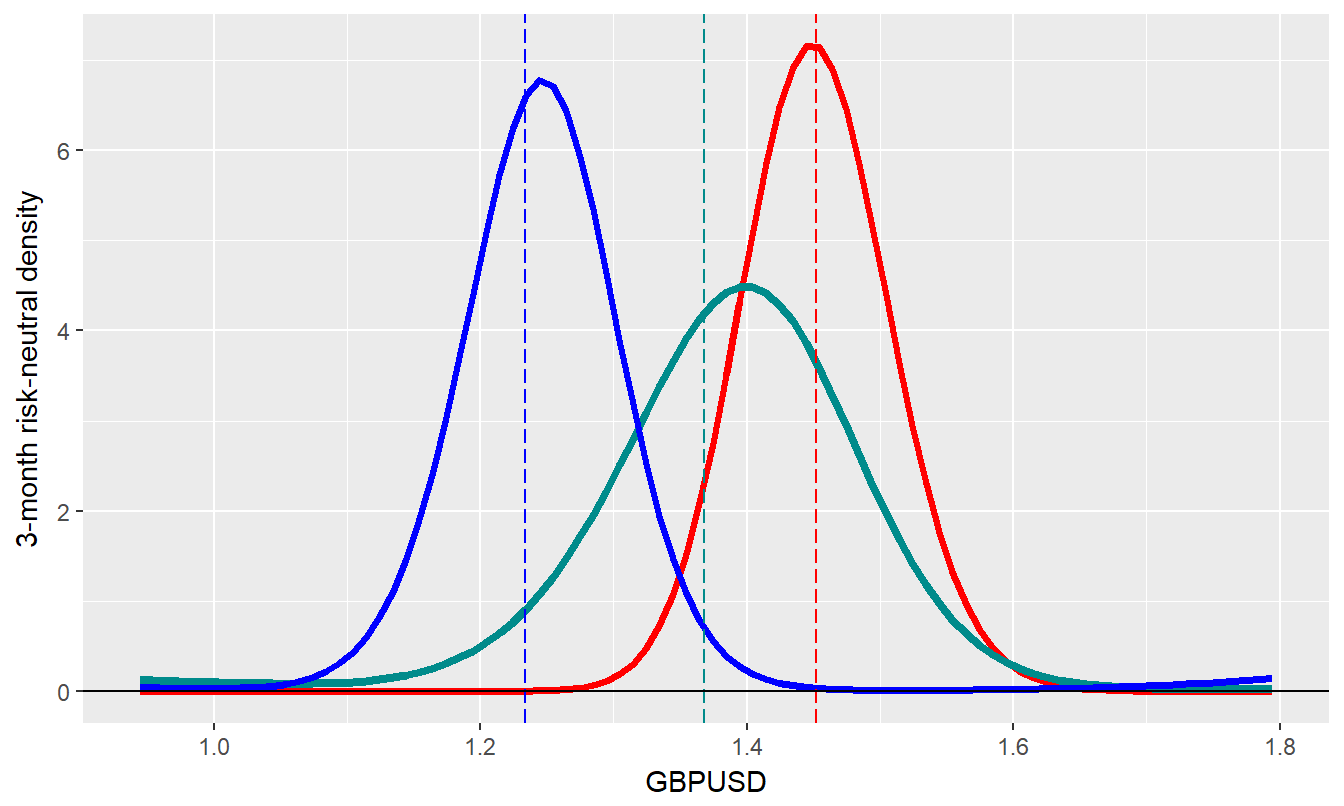
\includegraphics[width=1\linewidth]{images/unnamed-chunk-65-1} \caption{Shimnko risk neutral distributions.</br>Pre-Brexit: red; Brexit: cyan; post-Brexit: blue}\label{fig:unnamed-chunk-65}
\end{figure}

The pre-Brexit and Brexit exchange rate distributions are well behaved.
This is not the case for the post-Brexit distribution. Generally,
methods that use numerical differentiation could generate unstable or
misbehaved distributions when approximating the premium-strike function
or the implied volatility-strike function directly. Results improve
substantially when we generate the premium-strike curve from a fitted
implied volatility-delta curve.\footnote{See \citet{Malz1997} and
  \citet{Malz2014} for the specific case of FX options.}

\section{A graphical comparison of different
methods}\label{a-graphical-comparison-of-different-methods}

We start with the pre-Brexit distributions. Generate the plot with the
following commands:

\begin{Shaded}
\begin{Highlighting}[]
\KeywordTok{ggplot}\NormalTok{(}\DataTypeTok{data=}\NormalTok{shimko.rnd.df, }\KeywordTok{aes}\NormalTok{(}\DataTypeTok{x=}\NormalTok{Krange)) }\OperatorTok{+}\StringTok{ }
\StringTok{  }\KeywordTok{geom_line}\NormalTok{(}\KeywordTok{aes}\NormalTok{(}\DataTypeTok{y=}\NormalTok{shimko.rnd.preBrexit), }\DataTypeTok{col=}\StringTok{"red"}\NormalTok{, }\DataTypeTok{size=}\FloatTok{1.25}\NormalTok{) }\OperatorTok{+}
\StringTok{  }\KeywordTok{geom_line}\NormalTok{(}\DataTypeTok{data=}\NormalTok{gb.rnd.df, }\KeywordTok{aes}\NormalTok{(}\DataTypeTok{x=}\NormalTok{Krange, }\DataTypeTok{y=}\NormalTok{gb.rnd.preBrexit), }\DataTypeTok{col=}\StringTok{"darkcyan"}\NormalTok{, }\DataTypeTok{size=}\FloatTok{1.25}\NormalTok{) }\OperatorTok{+}
\StringTok{  }\KeywordTok{geom_line}\NormalTok{(}\DataTypeTok{data=}\NormalTok{ew.rnd.df, }\KeywordTok{aes}\NormalTok{(}\DataTypeTok{x=}\NormalTok{Krange, }\DataTypeTok{y=}\NormalTok{ew.rnd.preBrexit), }\DataTypeTok{col=}\StringTok{"blue"}\NormalTok{, }\DataTypeTok{size=}\FloatTok{1.25}\NormalTok{) }\OperatorTok{+}
\StringTok{  }\KeywordTok{geom_hline}\NormalTok{(}\DataTypeTok{yintercept=}\DecValTok{0}\NormalTok{, }\DataTypeTok{col=}\StringTok{"black"}\NormalTok{, }\DataTypeTok{size=}\FloatTok{0.5}\NormalTok{) }\OperatorTok{+}
\StringTok{  }\KeywordTok{labs}\NormalTok{(}\DataTypeTok{x=}\StringTok{"GBPUSD"}\NormalTok{, }\DataTypeTok{y=}\StringTok{"3-month risk-neutral density"}\NormalTok{)   }
\end{Highlighting}
\end{Shaded}

\begin{figure}
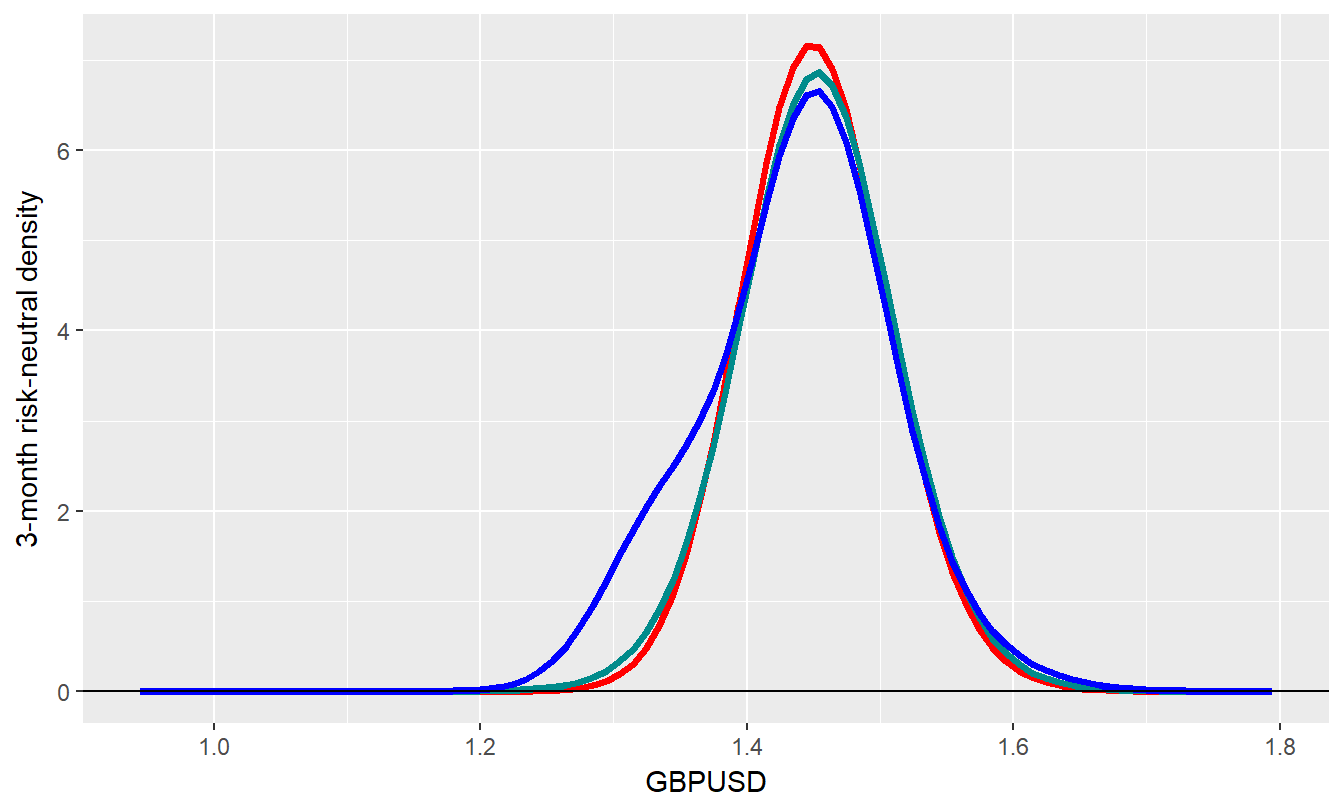
\includegraphics[width=1\linewidth]{images/unnamed-chunk-66-1} \caption{Pre-Brexit risk neutral distributions.</br>Generalized beta: cyan; Edgeworth expansion: blue; Shimko: red.}\label{fig:unnamed-chunk-66}
\end{figure}

The generalized beta distribution and Shimko methods generate very
similar pre-Brexit distributions. The Edgeworth expansion generates
fatter tails, especially in the left tail.

The Brexit distributions seem very different across methods (figure
below). The Edgeworth expansion again generates fatter left tails and
small negative probabilities in the right tail. The Shimko distribution
has thinner tails and less newness than the other two distributions.

\begin{Shaded}
\begin{Highlighting}[]
\KeywordTok{ggplot}\NormalTok{(}\DataTypeTok{data=}\NormalTok{shimko.rnd.df, }\KeywordTok{aes}\NormalTok{(}\DataTypeTok{x=}\NormalTok{Krange)) }\OperatorTok{+}\StringTok{ }
\StringTok{  }\KeywordTok{geom_line}\NormalTok{(}\KeywordTok{aes}\NormalTok{(}\DataTypeTok{y=}\NormalTok{shimko.rnd.Brexit), }\DataTypeTok{col=}\StringTok{"red"}\NormalTok{, }\DataTypeTok{size=}\FloatTok{1.25}\NormalTok{) }\OperatorTok{+}
\StringTok{  }\KeywordTok{geom_line}\NormalTok{(}\DataTypeTok{data=}\NormalTok{gb.rnd.df, }\KeywordTok{aes}\NormalTok{(}\DataTypeTok{x=}\NormalTok{Krange, }\DataTypeTok{y=}\NormalTok{gb.rnd.Brexit), }\DataTypeTok{col=}\StringTok{"darkcyan"}\NormalTok{, }\DataTypeTok{size=}\FloatTok{1.25}\NormalTok{) }\OperatorTok{+}
\StringTok{  }\KeywordTok{geom_line}\NormalTok{(}\DataTypeTok{data=}\NormalTok{ew.rnd.df, }\KeywordTok{aes}\NormalTok{(}\DataTypeTok{x=}\NormalTok{Krange, }\DataTypeTok{y=}\NormalTok{ew.rnd.Brexit), }\DataTypeTok{col=}\StringTok{"blue"}\NormalTok{, }\DataTypeTok{size=}\FloatTok{1.25}\NormalTok{) }\OperatorTok{+}
\StringTok{  }\KeywordTok{geom_hline}\NormalTok{(}\DataTypeTok{yintercept=}\DecValTok{0}\NormalTok{, }\DataTypeTok{col=}\StringTok{"black"}\NormalTok{, }\DataTypeTok{size=}\FloatTok{0.5}\NormalTok{) }\OperatorTok{+}
\StringTok{  }\KeywordTok{labs}\NormalTok{(}\DataTypeTok{x=}\StringTok{"GBPUSD"}\NormalTok{, }\DataTypeTok{y=}\StringTok{"3-month risk-neutral density"}\NormalTok{) }
\end{Highlighting}
\end{Shaded}

\begin{figure}
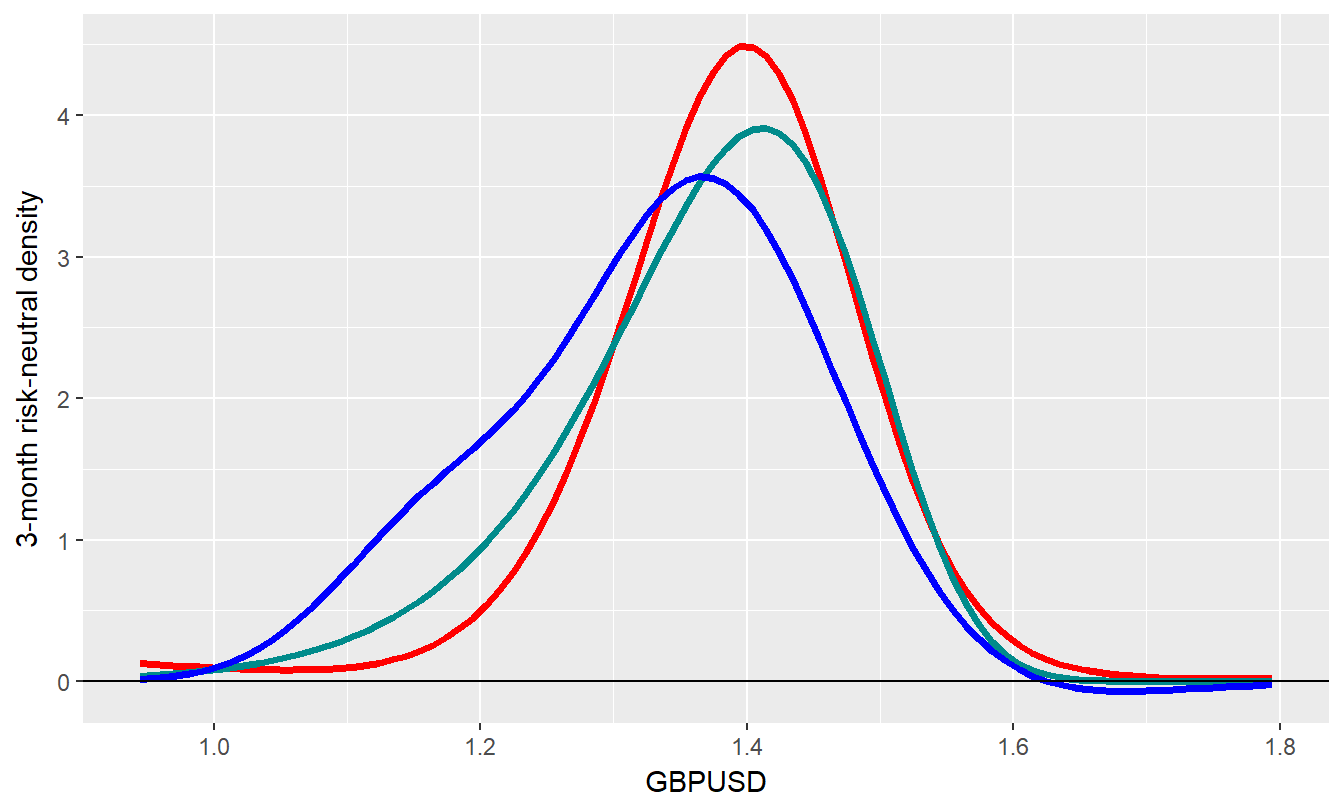
\includegraphics[width=1\linewidth]{images/unnamed-chunk-67-1} \caption{Brexit risk neutral distributions.</br>Generalized beta: cyan; Edgeworth expansion: blue; Shimko: red.}\label{fig:unnamed-chunk-67}
\end{figure}

Finally, we analyze the post-Brexit distributions (figure below). We
omit analyzing the Shimko distribution due to its counterintuitive
shape. For the GBP-USD pair, the Edgeworth expansion appears to be more
skewed and generate fatter left tails than the generalized beta
distribution.

\begin{Shaded}
\begin{Highlighting}[]
\KeywordTok{ggplot}\NormalTok{(}\DataTypeTok{data=}\NormalTok{shimko.rnd.df, }\KeywordTok{aes}\NormalTok{(}\DataTypeTok{x=}\NormalTok{Krange)) }\OperatorTok{+}\StringTok{ }
\StringTok{  }\KeywordTok{geom_line}\NormalTok{(}\DataTypeTok{data=}\NormalTok{gb.rnd.df, }\KeywordTok{aes}\NormalTok{(}\DataTypeTok{x=}\NormalTok{Krange, }\DataTypeTok{y=}\NormalTok{gb.rnd.postBrexit), }\DataTypeTok{col=}\StringTok{"darkcyan"}\NormalTok{, }\DataTypeTok{size=}\FloatTok{1.25}\NormalTok{) }\OperatorTok{+}
\StringTok{  }\KeywordTok{geom_line}\NormalTok{(}\DataTypeTok{data=}\NormalTok{ew.rnd.df, }\KeywordTok{aes}\NormalTok{(}\DataTypeTok{x=}\NormalTok{Krange, }\DataTypeTok{y=}\NormalTok{ew.rnd.postBrexit), }\DataTypeTok{col=}\StringTok{"blue"}\NormalTok{, }\DataTypeTok{size=}\FloatTok{1.25}\NormalTok{) }\OperatorTok{+}
\StringTok{  }\KeywordTok{geom_hline}\NormalTok{(}\DataTypeTok{yintercept=}\DecValTok{0}\NormalTok{, }\DataTypeTok{col=}\StringTok{"black"}\NormalTok{, }\DataTypeTok{size=}\FloatTok{0.5}\NormalTok{) }\OperatorTok{+}
\StringTok{  }\KeywordTok{labs}\NormalTok{(}\DataTypeTok{x=}\StringTok{"GBPUSD"}\NormalTok{, }\DataTypeTok{y=}\StringTok{"3-month risk-neutral density"}\NormalTok{)   }
\end{Highlighting}
\end{Shaded}

\begin{figure}
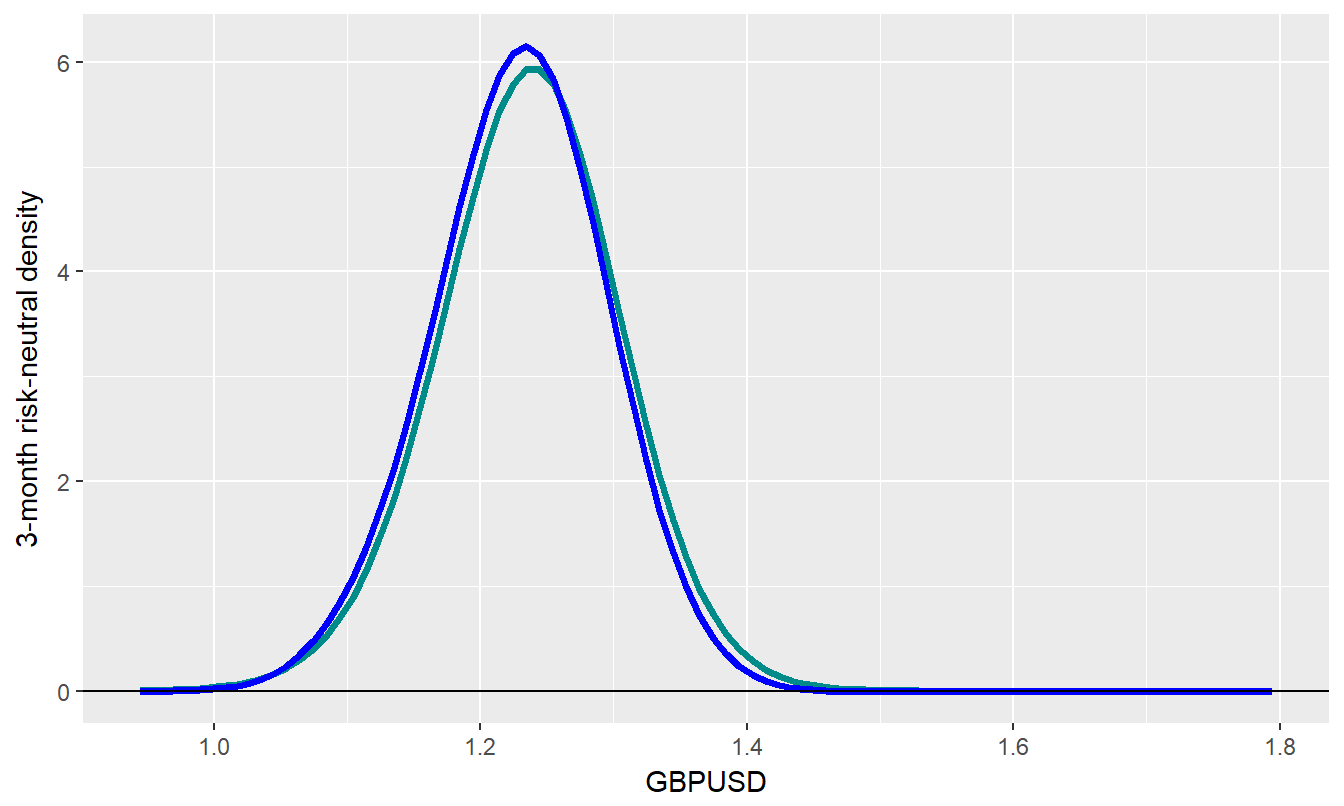
\includegraphics[width=1\linewidth]{images/unnamed-chunk-68-1} \caption{Post-Brexit risk neutral distributions.</br>Generalized beta: cyan; Edgeworth expansion: blue.}\label{fig:unnamed-chunk-68}
\end{figure}

\chapter{Epilogue}\label{epilogue}

With all calculations ready, it was time for Payne to wrap up its
analysis and to propose a small text box for the U.K. policy note. Once
it was ready, she send the draft to her manager, F.L. Atterman. Atterman
considered the box could be included in the note once Payne took on
board his editorial suggestions. It was not a bad outcome at all.
Atterman also suggested Payne to attempt to incorporate the FX option
information in a forecasting model. Payne wrote a note to enroll in the
internal forecasting courses offered by the Internal Cognitive
Development (ICD) department.

While walking back to her office Payne crossed paths with Huff. Although
he waved at her, she completely ignored him. ``No loss at all, as the
old man is no longer of any use,'' thought Payne. Her mind was already
busy strategizing on whom her coffee money and her time were better
spent in order to advance her career prospects.

\appendix


\chapter{Payne's policy note box}\label{paynes-policy-note-box}

 \textbf{Brexit: a FX options post-mortem}

Markets reacted strongly to the U.K.vote to leave the European Union in
June 2016. Ahead of the vote, the exchange rate had been declining
steadily from a peak of 1.7 USD/GBP in mid-2014 to around 1.4 USD/GBP at
the beginning of 2016 and held steady at that level during the first
half of 2016. In the week following the vote, however, the British pound
fell by more than ten percent against the U.S. dollar, reflecting partly
concerns about the decline of London as a major financial center.

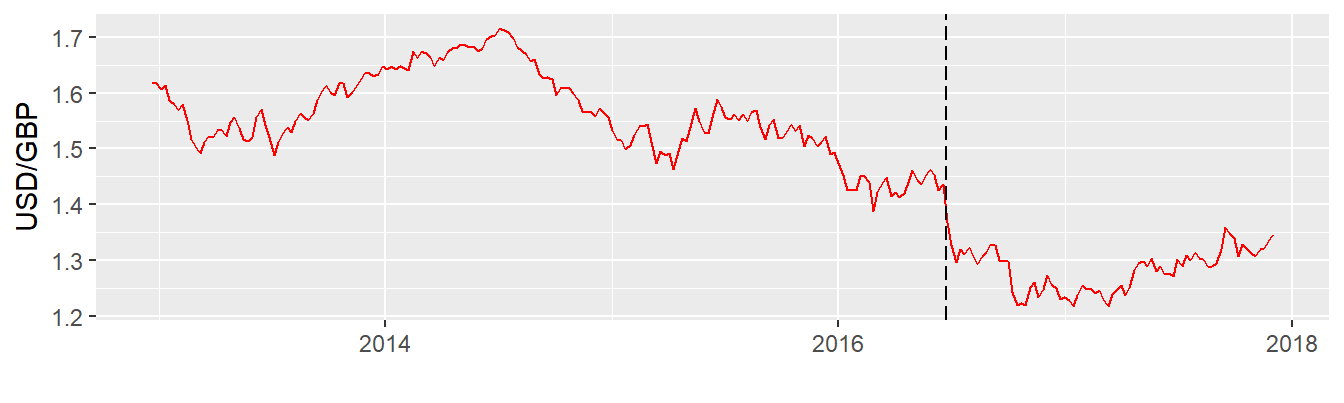
\includegraphics[width=1\linewidth]{images/unnamed-chunk-69-1}

The pound continued weakening during most of 2016, but started gaining
ground during most of 2017, rising to about 1.35 USD/GBP in December
2017 from as low as 1.2 USD/GBP in early 2017.

The strengthening of the pound in late 2017 may actually be hiding
weaknesses ahead for the British currency. This is evident from
violations in the covered interest parity relationship. By end-2017, the
widening differential between the US dollar rate implied in the forward
market the US dollar money market rate signals a strong demand for U.S.
dollars.

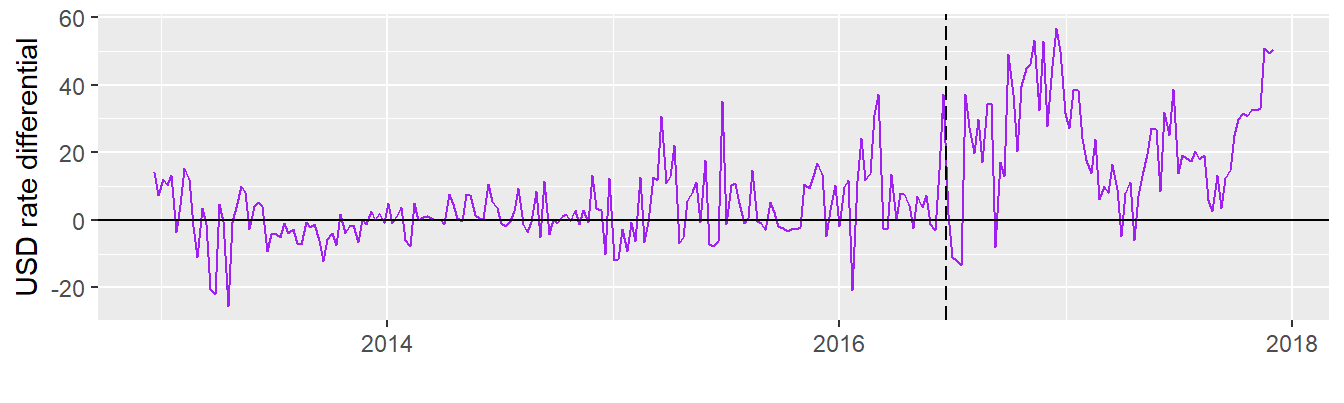
\includegraphics[width=1\linewidth]{images/unnamed-chunk-70-1}

The rate differential narrowed and almost vanished earlier in 2017 as
the Tories started losing their grip on power which culminated with
their loss of a parliamentary majority. Concerns about economic growth
prospects in the country, as outlined in the latest \emph{Inflation
Report}, appear to be driving the interest rate differential wider.

Although the exchange rate did not appear to anticipate the turmoil of
the Brexit vote, the FX options market had already started discounting
an unfavorable outcome to those in the stay camp. The value of risk
reversals, a combination of a short position on a put option with a long
position in a call option, is positive if markets are bullish on the
pound. When markets are bearish, the risk reversal is negative. Despite
the exchange rate fluctuating within a narrow range band, the 3-month 10
\(\Delta\) risk reversal contracts showed markets increasingly weighted
more large downside movements in the exchange rate than upside movements
ahead of the vote.

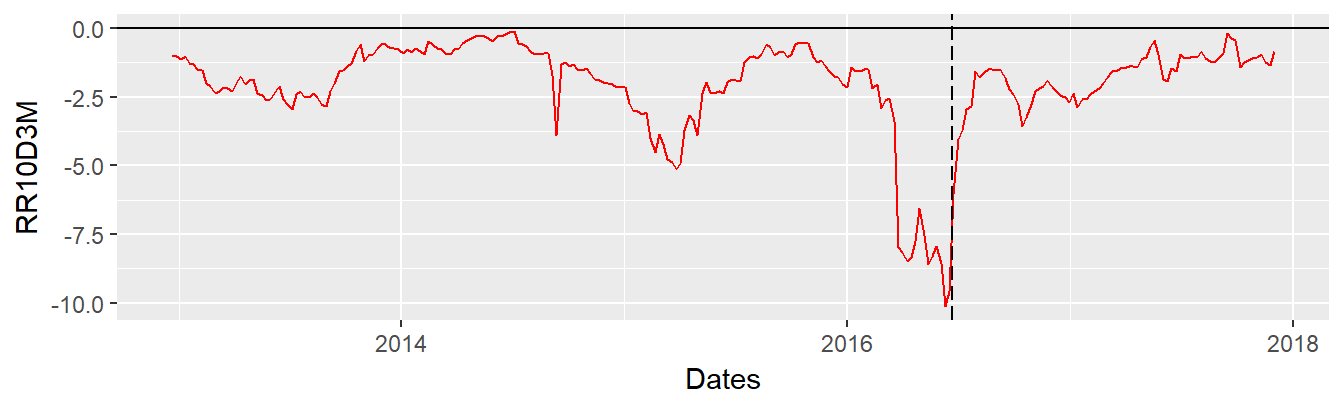
\includegraphics[width=1\linewidth]{images/unnamed-chunk-71-1} The
butterfly spread contracts complemented the information from the risk
reversal contracts. A positive contract value indicates that the
exchange rate is more likely to deviate significantly from its current
value. The deviations can be either positive or negative. The 3-month 10
\(\Delta\) butterfly spread contracts indicated large movements were
expected in early 2016. In combination of the risk reversals, the option
markets were revealing increased concerns about the impact of Brexit on
the exchange rate.

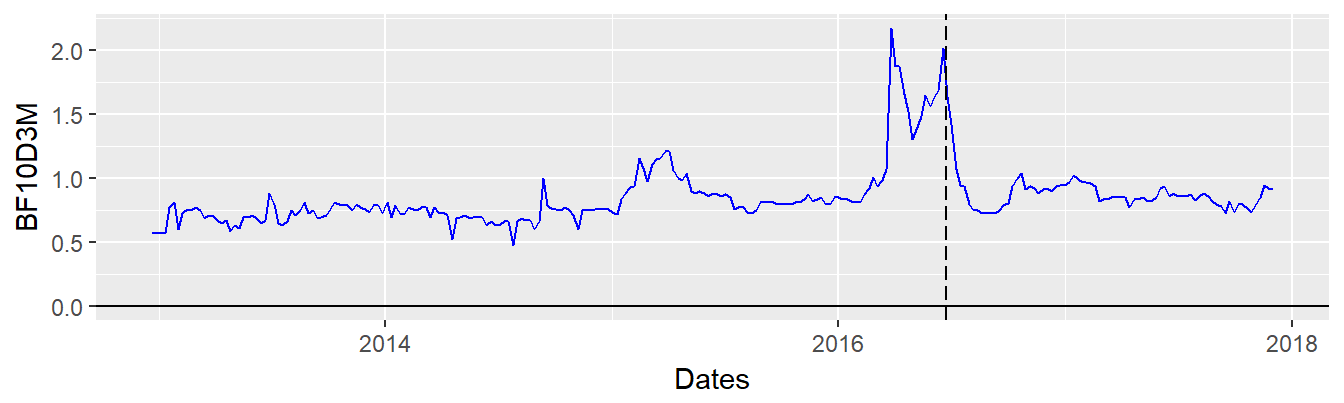
\includegraphics[width=1\linewidth]{images/unnamed-chunk-72-1} The
impact of the Brexit vote can be gauged directly from the 3-month
exchange rate probability distributions implied from option markets. The
red line shows the implied distribution as of January 8, 2016; and the
dark cyan line the distribution as of June 24, 2016. The vertical lines
show the respective spot exchange rates. The Brexit vote has turned
markets increasingly bearish on the British pound and some small but
positive weight was assigned to the event that the pound could trade at
par with the U.S. dollar.

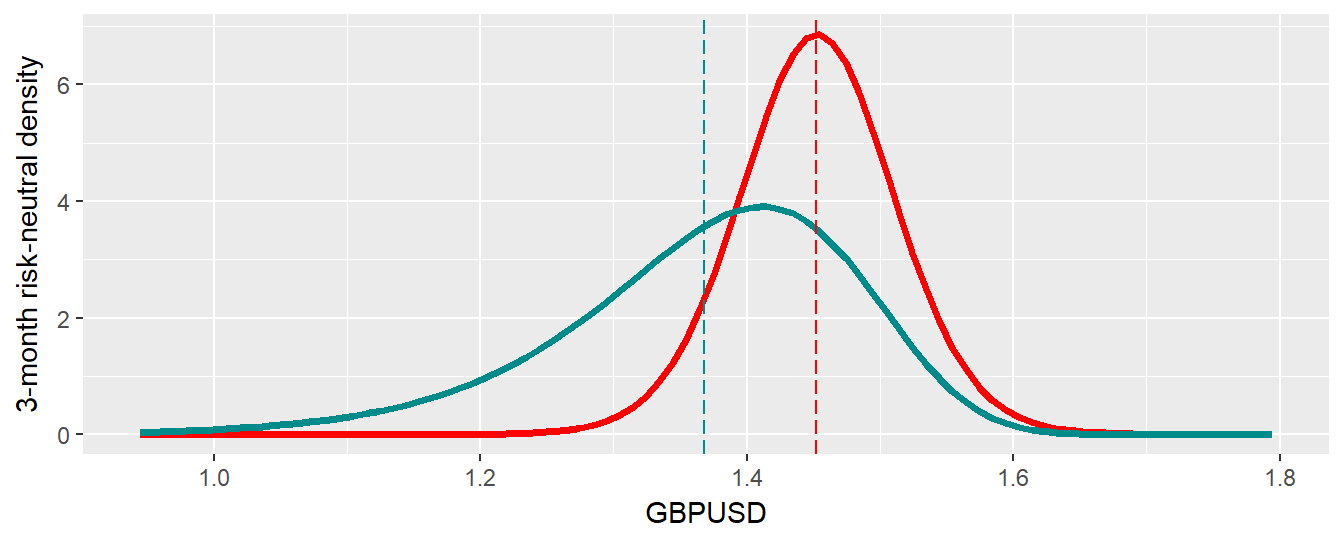
\includegraphics[width=1\linewidth]{images/unnamed-chunk-73-1}

As of December 1, 2017, market sentiment has stabilized as the
bearishness faded away as the probability distribution in blue shows.
Compared with the pre-Brexit distribution, the market considers that the
range of possible exchange rate realizations is narrower. Still, the
pound was still trading ten percent below its level just before the
Brexit vote, and the violation of covered interest parity justifies
increased vigilance.

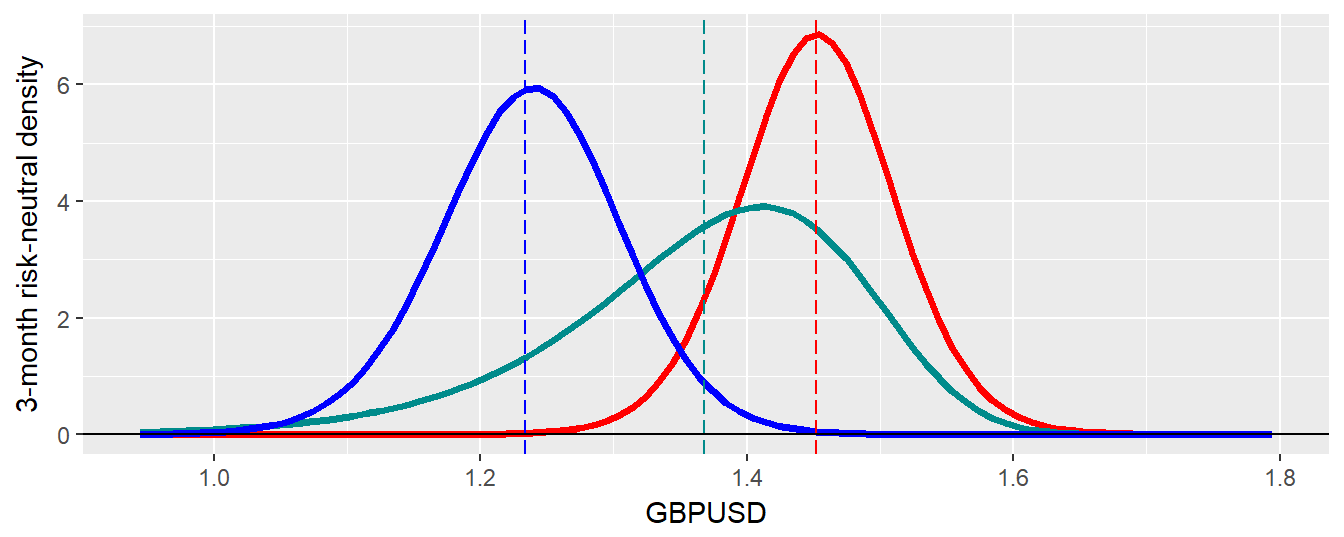
\includegraphics[width=1\linewidth]{images/unnamed-chunk-74-1}

\chapter{Bloomberg Training Video}\label{bloomberg-training-video}

Bloomberg is one of the main providers of financial data, including
price quotes for the FX option contracts discussed in these notes. The
video below provides an overview of the FX option functionality
available in the Bloomberg terminals, including the rapid generation of
volatility smiles and volatility surfaces.

\url{https://youtu.be/wpcvGhYN4eQ}

\bibliography{thepackages,thebook}


\end{document}
